\documentclass[10pt,a4paper,openany,twoside]{book}
%-------------------------------------宏包引用---------------------------------------------------
\usepackage[paperwidth=155mm,paperheight=230mm,textheight=170mm,textwidth=110mm,left=20mm,right=25mm, top=35mm, bottom=25mm]{geometry}            %定义版面
%--------------------------------------------------------------------------------------
\usepackage{fontspec}
\usepackage{xunicode}
\usepackage{xltxtra}
\usepackage[slantfont,boldfont]{xeCJK}
%--------------------------------------------------------------------------------------
\usepackage[listings,theorems]{tcolorbox}
\usepackage{fancybox}                 % 边框,有阴影,fancybox提供了五种式样\fbox,\shadowbox,\doublebox,\ovalbox,\Ovalbox。
\usepackage{colortbl}                   % 单元格加背景
\usepackage{fancyhdr}                 % 页眉和页脚的相关定义
\usepackage[CJKbookmarks, colorlinks, bookmarksnumbered=true,pdfstartview=FitH,linkcolor=black]{hyperref}   % 书签功能,选项去掉链接红色方框
\usepackage{tabularx}
\usepackage{tcolorbox}
%\usepackage{ctex,ctexcap}

%-----------------------------源代码---------------------------------------------------------
\usepackage{listings}
\usepackage{lineno}

%--------------------线条加粗-------------------
\usepackage{booktabs}
\usepackage{multirow}

%-------------------caption字体----------------
\usepackage[font=footnotesize]{caption}

\usepackage{scrextend}

%--------------------折现图------------------
\usepackage{tikz}
\usepackage{pgfplots}

   %引用宏包所在位置
%-----------------------------------------------------主文档 格式定义---------------------------------
\addtolength{\headsep}{-0.1cm}        %页眉位置
%\addtolength{\footskip}{0.4cm}       %页脚位置

\changefontsizes{9pt}
%-----------------------------------------------------设定字体等------------------------------
\setmainfont{Times New Roman}    % 缺省字体

\setCJKmainfont{SimSun}
\setCJKsansfont{SimHei}
\setCJKmonofont{FangSong}
\setCJKfamilyfont{song}{SimSun}
\setCJKfamilyfont{hei}{SimHei}
\setCJKfamilyfont{kai}{KaiTi}
\setCJKfamilyfont{fs}{FangSong}
\setCJKfamilyfont{li}{LiSu}
\setCJKfamilyfont{you}{YouYuan}
%\setCJKfamilyfont{yahei}{Microsoft YaHei}
%\setCJKfamilyfont{xingkai}{STXingkai}
\setCJKfamilyfont{xinwei}{STXinwei}
\setCJKfamilyfont{fzyao}{FZYaoTi}
\setCJKfamilyfont{fzshu}{FZShuTi}
%-------------------------------------------------------------------
\newCJKfontfamily\song{SimSun}
\newCJKfontfamily\hei{SimHei}
\newCJKfontfamily\kai{KaiTi}
\newCJKfontfamily\fs{FangSong}
\newCJKfontfamily\li{LiSu}
\newCJKfontfamily\you{YouYuan}
\newCJKfontfamily\yahei{Microsoft YaHei}
%\newCJKfontfamily\xingkai{STXingkai}
\newCJKfontfamily\xinwei{STXinwei}
\newCJKfontfamily\fzyao{FZYaoTi}
\newCJKfontfamily\fzshu{FZShuTi}
%-----------------------------------------------------------定义颜色---------------
\definecolor{black}{rgb}{0.0, 0.0, 0.0}
\definecolor{grey}{rgb}{0.9,0.9,0.9}
\definecolor{blueblack}{cmyk}{0,0,0,0.35}%浅黑
\definecolor{darkblue}{cmyk}{1,0,0,0}%纯蓝
\definecolor{lightblue}{cmyk}{0.15,0,0,0}%浅蓝

%------------------------listings代码格式--------------------------
\lstset{language=C,tabsize=4,keepspaces=true,
	breakindent=22pt, 
	numbers=left,stepnumber=1,numberstyle=\footnotesize,
	basicstyle=\small,
	showspaces=false,
	flexiblecolumns=true,
	breaklines=true,breakautoindent=true,breakindent=4em,
	extendedchars=false,
	%frame=tb,
	escapeinside=``
}

%------------------------折线图格式-----------------------------
\pgfplotsset{every axis legend/.style={
cells={anchor=west},
draw=black,
at={(0.2,0.8)}
}}

%-----------------------------------------------------------定义、定理环境-------------------------
\newcounter{myDefinition}[chapter]\def\themyDefinition{\thechapter.\arabic{myDefinition}}
\newcounter{myTheorem}[chapter]\def\themyTheorem{\thechapter.\arabic{myTheorem}}
\newcounter{myCorollary}[chapter]\def\themyCorollary{\thechapter.\arabic{myCorollary}}

\tcbmaketheorem{defi}{定义}{fonttitle=\bfseries\upshape, fontupper=\slshape, arc=0mm, colback=lightblue,colframe=darkblue}{myDefinition}{Definition}
\tcbmaketheorem{theo}{定理}{fonttitle=\bfseries\upshape, fontupper=\slshape, arc=0mm, colback=lightblue,colframe=darkblue}{myTheorem}{Theorem}
\tcbmaketheorem{coro}{推论}{fonttitle=\bfseries\upshape, fontupper=\slshape, arc=0mm, colback=lightblue,colframe=darkblue}{myCorollary}{Corollary}
%------------------------------------------------------------------------------
\newtheorem{proof}{\indent\hei \textcolor{darkblue}{证明}}
\newtheorem{Solution}{\indent\hei \textcolor{darkblue}{解}}
%------------------------------------------------定义页眉下单隔线----------------
\newcommand{\makeheadrule}{\makebox[0pt][l]{\color{black}\rule[.7\baselineskip]{\headwidth}{0.3pt}}\vskip-.8\baselineskip}

%-----------------------------------------------定义页眉下双隔线----------------
\makeatletter
\renewcommand{\headrule}{{\if@fancyplain\let\headrulewidth\plainheadrulewidth\fi\makeheadrule}}
\pagestyle{fancy}
\renewcommand{\chaptermark}[1]{\markboth{第\chaptername 章\quad #1}{}}    %去掉章标题中的数字
\renewcommand{\sectionmark}[1]{\markright{\thesection\quad #1}{}}    %去掉节标题中的点
\fancyhf{} %清空页眉
\fancyhead[RO]{\kai{\footnotesize.~\color{black}\thepage~.}}         % 奇数页码显示左边
\fancyhead[LE]{\kai{\footnotesize.~\color{black}\thepage~.}}         % 偶数页码显示右边
\fancyhead[CO]{\song\footnotesize\color{black}\rightmark} % 奇数页码中间显示节标题
\fancyhead[CE]{\song\footnotesize\color{black}\leftmark}  % 偶数页码中间显示章标题
%---------------------------------------------------------------------------------------------------------------------


    %格式所在位置
\begin{document}
%\pagenumbering{Roman}    %Roman字体书写页码
%---------------------------------------------------封面等-----------------------

% ------------------------------封面-----------------------------------------------
% -----------------------------------------------------------------------------------
\title{{\Huge 操作系统}\\{\LARGE Three Easy Pieces}}
\author{Johnnie Xu ~~ 落忧\hspace{1em}译}
\date{\vspace*{3cm}\centering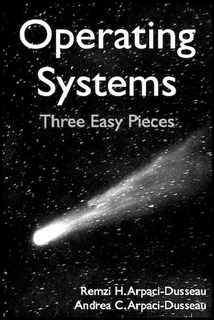
\includegraphics[totalheight=1.5in]{fig/operating-systems.jpeg}\\武汉 $\cdot$ 常州}
\maketitle
% -----------------------------------------------------------------------------------
                         %封面
\include{preface/intro}                          %简介
%\markboth{序}{序} \vspace*{0.0cm}
\thispagestyle{empty}
\vspace*{2.2cm}
\centerline{\zihao{2}\hei{\color{darkblue}{第二版序}}}\vspace{2cm}

吕同富教授编著的《数值计算方法》
………………………………………………


\vspace{2cm}

\hfill XXXXXX\hspace{0.2em}

\hfill 2012年08月于XXXXXX\hspace{0.2em}
                        %序
\markboth{致教育工作者}{致教育工作者} \vspace*{0.0cm}
\thispagestyle{empty}
%\vspace*{2.2cm}
\centerline{\hei{\Large 致教育工作者}}\vspace{2cm}

如果你是希望使用本书的讲师或教授,随时欢迎。可能你已经注意到,本书是免费的,且可以从下面网页中获取:\\
http://www.ostep.org\\
你也可以从lulu.com网站购买纸质版。请在上述网页上查询。

本书的推荐引用格式(截止至目前)如下:\\
~~~~Operating Systems: Three Easy Pieces\\
~~~~Remzi H. Arpaci-Dusseau and Andrea C. Arpaci-Dusseau\\
~~~~Arpaci-Dusseau Books, Inc.\\
~~~~May, 2014 (Version 0.8)\\
~~~~http://www.ostep.org\\

这个课程分成一个学期15周比较好,这样可以覆盖书中的大部分话题,也能达到比较适中的深度。要是把本课程压缩到10周的话,可能需要每个部分都舍弃一些细节。还有一些关于虚拟机监控器的章节,通常压缩到虚拟化的结尾部分或者作为一个aside放在最后。

许多操作系统的书都会将并发性部分放在前面,本书不太一样,将其放在了虚拟化部分之后,这样在此之前可以对CPU和内存的虚拟化有一定理解。从我们15年教授此课程的经验来看,如果学生们没有理解地址空间是什么,进程是什么,或者上下文切换会在任意时间发生,他们都会有个困惑期——不知道并发性问题是如何引起的,为什么要试图解决这个问题。然而,一旦他们理解了虚拟化中的那些概念,当介绍线程和由线程引起的问题时会变得很简单,起码会简单些。

你可能注意到本书没有与之对应的幻灯片。主要原因是我们相信这个过时的教学方法:粉笔和黑板。因此,当我们在讲授这门课程时,我们脑子里带几个主要的思想和一些例子到课堂上,用板书的形式呈现给学生;讲义以及现场编写演示代码也是很有用的。在我们的经验里,使用太多的幻灯片会使得学生心思不在课堂上,因为他们知道反正资料就在这里,可以以后慢慢消化;板书的话会使得课堂像一个现场观看体验,因此会更有互动性、动态性,也会使学生们更好的享受你的课。

如果你想要一份我们上课的笔记的话,可以给我们发邮件。我们已经共享给了全世界很多老师。

最后一个请求:如果你使用网页上的免费章节,请仅仅链接到他们,而不是拷贝到本地。这会帮助我们追踪这些章节的使用情况(过去几年里已经有超过一百万的章节下载量),也可以确保学生们获得的是最新最好的版本。
                   	    %前言
\markboth{致学生}{致~学~生} \vspace*{0.0cm}
\thispagestyle{empty}
%\vspace*{2.2cm}
\centerline{\hei{\Large 致~~学~~生}}\vspace{2cm}

如果你是正在阅读本书的学生,谢谢你!我们很荣幸能够为你提供一些材料帮助你求索关于操作系统的知识。我们俩都很怀念本科时候的一些教科书(如:Hennessy and Patterson [HP90],计算机系统结构的一本经典书),当然也希望本书能够带给你一个美好回忆。

你也许注意到本书是免费的,在网上可以获取到。其主要原因是:教科书一般都比较贵。我们希望,本书能够成为免费书籍新浪潮的第一人,以帮助那些追求自己学业的人。无论他们来自世界的哪个地方或者他们愿意为一本书花多少钱。如若不然,这本免费书也聊胜于无。

可能的话,我们还希望给你们指出书中许多材料的原始出处:那些多年来塑造了操作系统领域的重要的论文和人物。思想不会凭空产生,他们来自于聪明又努力的人(包括许多图灵奖获得者\footnote{图灵奖是计算机科学领域的最高奖;就像诺贝尔奖一样。}),因此我们应该尽可能的去纪念这些思想和人物。在纪念他们时,我们非常希望在写本书时能更好地理解已经发生的革命,而不是仿佛这些思想一直都存在似的[K62]。再者,或许这些参考文献能够促进你自己去更深的挖掘;阅读著名的论文是这个领域最好的学习方法之一。


                     %前言
\markboth{最后的话}{最后的话} \vspace*{0.0cm}
\thispagestyle{empty}
%\vspace*{2.2cm}
\centerline{\hei{\Large 最~后~的~话}}\vspace{2cm}

Yeats【W. B. Yeats,威廉.巴特勒.叶慈】有句名言:”教育不是注满一桶水,而是点燃一把火。”他既是对的但同时也是错的\footnote{如果他确实说了这句话;如许多名人名言一样,这句话的历史也不明}。你必须”注满那桶水”,这些笔记正好在此帮助你的学业;毕竟,当你去Google面试,他们问你一个关于如何使用信号量的刁钻问题,最好还是真的知道信号量是什么,对吧!

但是叶慈的重点明显是:教育真正的关键在于使你能对某样事务产生兴趣,去学习一些自己觉得更重要的东西,而不仅仅是某些课程中为了得高分而需消化的东西。Remzi的父亲曾经说过:”走出课堂学习”。

我们撰写了这些笔记来激发你对操作系统的兴趣,从而去围绕这个话题自己做更多的阅读,去跟你的教授讨论这个领域正在进行的有意思的研究,甚至参与到这个研究中来。这是一个很伟大的领域,充满了精彩美妙思想,它们以深刻而重要的方式塑造了计算机历史。我们知道虽然这把火不能燃烧你们所有人,至少我们希望能够燃烧你们一部分人,甚至几个人。因为一旦这把火被点燃了,那就是你们真正可以做一些伟大事情的时候。教育过程的真正关键是:行动,去研究新的有趣的话题,去学习,去成长,还有最重要的是去寻找能够点燃你的事情。


\vspace{1cm}

\hfill JAndrea and Remzi\hspace{0.2em}

\hfill Married couple \hspace{0.2em}

\hfill Professors of Computer Science at the University of Wisconsin\hspace{0.2em}

\hfill Chief Lighters of Fires, hopefully\footnote{如果这个听起来我们如纵火犯一样在承认一些历史的话,那你可能抓错重点了。也许,如果这听起来俗气的话,那好,因为他就是这么俗气,但你门不得不为此原谅我们。}\hspace{0.2em}


\section*{致谢}
这一节包含了我们对那些帮助撰写本书的人的感谢。现在最重要的事情:你们的名字在这里找到!但是,你一定要帮忙。所以给我们发送一些反馈并帮助我调试本书吧。你可能会出名!或者至少你的名字会出现在本书中。

到目前为止,帮助过本书的人包括: Abhirami Senthilkumaran*, Adam Drescher* (WUSTL), Adam Eggum, Ahmed Fikri*, Ajaykrishna Raghavan, Akiel Khan, Alex Wyler, Anand Mundada, B. Brahmananda Reddy (Minnesota), Bala SubrahmanyamKambala, Benita Bose, BiswajitMazumder (Clemson), Bobby Jack, Bj ¨orn Lindberg, Brennan Payne, Brian Kroth, Cara Lauritzen, Charlotte Kissinger, Chien-Chung Shen (Delaware)*, Christoph Jaeger, Cody Hanson, Dan Soendergaard (U. Aarhus), David Hanle (Grinnell), Deepika Muthukumar, Dorian Arnold (NewMexico), DustinMetzler, Dustin Passofaro, Emily Jacobson, EmmettWitchel (Texas), Ernst Biersack (France), Finn Kuusisto*, Guilherme Baptista, Hamid Reza Ghasemi, Henry Abbey, Hrishikesh Amur, Huanchen Zhang*, Hugo Diaz, Jake Gillberg, James Perry (U.Michigan-Dearborn)*, Jan Reineke (Universit¨at des Saarlandes), Jay Lim, Jerod Weinman (Grinnell), Joel Sommers (Colgate), Jonathan Perry (MIT), Jun He, Karl Wallinger, Kartik Singhal, Kaushik Kannan, Kevin Liu*, Lei Tian (U.Nebraska-Lincoln), Leslie Schultz, LihaoWang, MarthaFerris,Masashi Kishikawa (Sony), Matt Reichoff, Matty Williams, Meng Huang, Mike Griepentrog, Ming Chen (Stonybrook),Mohammed Alali (Delaware),Murugan Kandaswamy, Natasha Eilbert, Nathan Dipiazza, Nathan Sullivan, Neeraj Badlani (N.C. State),
Nelson Gomez, NghiaHuynh (Texas), Patricio Jara, Radford Smith, RiccardoMutschlechner, Ripudaman Singh, Ross Aiken, Ruslan Kiselev, Ryland Herrick, Samer AlKiswany, SandeepUmmadi (Minnesota), Satish Chebrolu (NetApp), Satyanarayana Shanmugam*, Seth Pollen, Sharad Punuganti, Shreevatsa R., Sivaraman Sivaraman*, Srinivasan Thirunarayanan*, Suriyhaprakhas BalaramSankari, SyJinCheah, Thomas Griebel, Tongxin Zheng, Tony Adkins, Torin Rudeen (Princeton), Tuo Wang, Varun Vats, Xiang Peng, Xu Di, Yue Zhuo (Texas A\&M), Yufui Ren, Zef RosnBrick, Zuyu Zhang.

特别感谢Joe Meehean教授(Lynchburg)对每一章的详细注释,Jerod Weinman教授(Grinnell)以及他整个班级不可思议的手册,Chien-Chung Shen教授(Delaware)宝贵细致的阅读和意见,以及Adam Drescher(WUSTL)的仔细阅读和建议。以及所有在资料细化中极大帮助过这些作者的所有人。

同时,也感谢这些年修过537课程的数百名学生。特别的,感谢促使这些笔记第一次成为书面形式的08年秋季班(他们苦于没有任何可阅读的教材——都是有进取心的学生!),并通过赞扬他们使我们能坚持下来(包括那年课程评价里令人捧腹的评价”ZOMG!{典故}你应该写一本全新的教材!")。

当然也亏欠了几个勇敢参与了xv6项目的实验课程的几个人的感谢,其中许多现在已经纳入饿了537主课程中。09年春季班: Justin Cherniak, Patrick Deline, Matt Czech, Tony Gregerson, Michael Griepentrog, Tyler Harter, Ryan Kroiss, Eric Radzikowski, Wesley Reardan, Rajiv Vaidyanathan, and Christopher Waclawik。09年秋季班: Nick Bearson, Aaron  Brown, Alex Bird, David Capel, Keith Gould, Tom Grim, Jeffrey Hugo, Brandon Johnson, John Kjell, Boyan Li, James Loethen,Will McCardell, Ryan Szaroletta, Simon Tso, and Ben Yule.10年春季班: Patrick Blesi, Aidan Dennis-Oehling, Paras Doshi, Jake Friedman, Benjamin Frisch, Evan Hanson, Pikkili Hemanth, Michael Jeung, Alex Langenfeld, Scott Rick, Mike Treffert, Garret Staus, Brennan Wall, Hans Werner, Soo-Young Yang, and Carlos Griffin (almost).

尽管我们的研究生学生没有直接帮助本书的撰写,但是他们教会了我们很多关于这个系统的东西。他们在Wisconsin时,我们经常与他们交流,他们做了所有的实际的工作。并且通过汇报他们做的事情,每周我们也学到了很多新的东西。这个名单包括我们收集到的目前和以前已经发表过论文的学生,星号标记表示那些在我们指导下获得了博士学位的学生: Abhishek Rajimwale, Ao Ma, Brian Forney, Chris Dragga, Deepak Ramamurthi, Florentina Popovici*, Haryadi S. Gunawi*, James Nugent, John Bent*, Lanyue Lu, Lakshmi Bairavasundaram*, Laxman Visampalli, Leo Arulraj, Meenali Rungta,Muthian Sivathanu*, Nathan Burnett*, Nitin Agrawal*, Sriram Subramanian*, Stephen Todd Jones*, Suli Yang, Swaminathan Sundararaman*, Swetha Krishnan, Thanh Do, Thanumalayan S. Pillai, Timothy Denehy*, Tyler Harter, Venkat Venkataramani, Vijay Chidambaram, Vijayan Prabhakaran*, Yiying Zhang*, Yupu Zhang*, Zev
Weiss.

最后还欠Aaron Brown一个感激之情,他多年前第一个带了这门课(09年春),然后有带了xv6实验课(09年秋),最后担任了本课程的研究生助教两年左右(10年秋至12年春)。他的辛勤工作极大的促进了项目的进展(特别是基于xv6的),并因此帮助了Wisconsin的无数的本科生和研究生优化可学习体验。正如Aaron想说的(他一贯的简洁风格):”Thx."

\vspace{1cm}

\hfill Johnnie Xu\hspace{0.2em}

\hfill ****@**** \hspace{0.2em}

\hfill 2015年01月\hspace{0.2em}

%\include{preface/c_abstract}             %中文摘要
%\include{preface/e_abstract}             %英文摘要
%-------------------------------------目录部分------------------------------------------
\setcounter{page}{1}   %重新开始页码
\renewcommand\contentsname{目\qquad 录}
%-------------------下面三行去掉了目录首页页码---------------------
\makeatletter
\let\ps@plain\ps@empty
\makeatother
%-------------------------------------------------------------------------
\tableofcontents                                    %目录
%\addtocontents{toc}{\protect\begin{multicols}{2}}       %目录分两栏开始
\mainmatter    %前言和目录页码结束,正文重新开始设置页码
%-----------------------------------------正文开始------------------------------
\chapter{本书的一段对话}
\thispagestyle{empty}


\textbf{教授:}欢迎来到这本书!它叫作\textbf{操作系统的三条简洁之道},我在这里会教你们一些你必须了解的操作系统知识。我是「教授」;你们呢?\newline
\textbf{学生:}你好,教授!我是「学生」,你应该猜到了。我在这里准备向您学习。\newline
\textbf{教授:}听起来不错。有什么问题不?\newline
\textbf{学生:}当然,为什么这本书叫作『三条简洁之道』呢?\newline
\textbf{教授:}很简单,你看,这是物理学家理查德·费曼的课程……\newline
\textbf{学生:}哦,是那位写了『别闹了,费曼先生』的那个人吗?好书,这本书是不是也会像那本书一样幽默?\newline
\textbf{教授:}额,不是的。那本书的确很不错,我很高兴你读过那本书。这本书更像他在物理学上的笔记。一些基础被定义为归纳为『六条简洁之道』。他是讨论的物理方面的知识;而我们是讨论以计算机为主题的『三条简洁之道』。差不多,操作系统正好是物理学一半的难度。\newline
\textbf{学生:}那真好,我也喜欢物理。是哪些简洁之道呢?\newline
\textbf{教授:}我们将会学到计算机的三个关键点:『\textbf{虚拟化,并发,持久化}』。在学习这些知识点的时候,我们会了解整个操作系统是如何运作的,包括 CPU 如何决定下一个运行什么程序。如何将内存载入到虚拟内存中。虚拟机监控如何运作,怎样管理硬盘信息,以及一些如何构建部分掉线但仍然可以工作的分布式系统。这是这些东西的主要顺序。\newline
\textbf{学生:}我对您说的这些还没什么概念。\newline
\textbf{教授:}很好,那说明你上对了课了。\newline
\textbf{学生:}我还有另外一个问题:学这些东西最好的方法是什么?\newline
\textbf{教授:}问的好!每个人都需要了解这些,当然,我会这样做:去上课,听教授介绍材料。然后到周末阅读自己的笔记,来帮助你的大脑更深入的理解。一段时间后(提示:在考试之前),再阅读这些笔记来牢固知识。当然,你的教授肯定会布置一些作业和项目,你必须完成;尤其是做项目的时候你为了解决问题而写的代码,是实践笔记中的知识最好的方式。孔子曾经说过……\newline
\textbf{学生:}哦,我知道!『不闻不若闻之,闻之不若见之,见之不若知之,知之不若行之。学至于行之而止矣。』是这句或者类似的吧。\newline
\textbf{教授:}(惊讶)你怎么知道我想说的呢?\newline
\textbf{学生:}因为接下去就像这句啊。而且我非常崇拜孔子,更加崇拜荀子。此句应该是荀子所言。\newline
\textbf{教授:}(震惊)好吧,我想我们要一起好好的努力了。真正的加油。\newline
\textbf{学生:}教授——如果可以的话,我还剩一个问题。这段对话是做什么用的啊?我的意思是,这不应该是一本书吗?为什么不直接介绍实质性的东西呢?\newline
\textbf{教授:}嗯,好问题,好问题!我认为和你自己单独聊这些和思考问题更有用,这段对话就是为了这个。所以你和我要一起工作来完成这个复杂的点子。你准备好了吗?\newline
\textbf{学生:}那我们必须思考?好吧,我准备好了。我的意思是,有一些其他的我能做的吗?貌似我在这本书之外没有太多的出场机会。\newline
\textbf{教授:}不幸的是,我也没有。好了,我们开始工作吧。       %第一章
\chapter{操作系统介绍}
\thispagestyle{empty}       %第二章
%\include{book/chap3}       %第三章
%\include{book/chap4}       %第四章
%\include{book/chap5}       %第五章
%\include{book/chap6}       %第六章
%\include{book/chap7}       %第七章
%\include{book/chap8}       %第八章
%\include{book/chap9}       %第九章
\chapter{并发性简介}
\thispagestyle{empty}

%\section{引言}
到目前为止,我们已经知道了操作系统基本执行部件的抽象概念的发展。我们已经了解如何『使用』单个物理CPU并将其抽象成多个虚拟CPU,因此多个程序看似同时运行成为了可能【注:在单个单核CPU上,同一时刻实际上只有一个程序在运行】。我们也学习了如何为每个进程构建一个看似很大且私有的虚拟内存;地址空间的抽象概念让每一个程序都好像有了自己的内存,而实际上是操作系统暗地里跨物理内存复用了地址空间(有时是磁盘)。

本节,我们将为单个正在运行的进程引入一个新的概念:线程。不像先前一个程序内只有一个执行点的视角(只从一个PC寄存器取指令和执行指令),一个多线程程序不止一个执行点(多个PC寄存器,可以从每一个PC取指令和执行指令)。从另一个角度来思考这个问题,每一个线程很像一个独立的进程,但是与进程的区别是:进程内的各个线程共享相同的地址空间。所以各个线程可以访问相同的数据。

单个线程的状态与进程的状态的很类似,有一个程序计数器(PC)来跟踪程序从何处取指令。每个线程有自己的用于计算的寄存器集;因此,如果在单个处理器上运行着两个线程,当从一个线程(T1)切换到另一个线程(T2)时,就会发生一次上下文切换。线程的上下文切换跟进程的上下文切换很类似,因为需要保存T1的寄存器状态,并在T2运行之前加载T2的寄存器状态。对于进程来说,我们将状态保存到进程控制块(process control block,PCB);对于线程来说,我们需要一个或多个线程控制块(thread control blocks,TCBs)来存储单个进程中的多个线程的状态。尽管如此,线程间的上下文切换比起进程来,有一个重要区别:地址空间依旧保持不变(没有必要切换正在使用的页表)。

线程与进程之间的另一个重要的区别是栈(stack)。在经典进程(现在可以称之为单线程进程,single-threaded process)地址空间的简单模型中,有一个单独的栈,通常位于地址空间的的底端(见下左图)。

\begin{figure}[h]
\centering
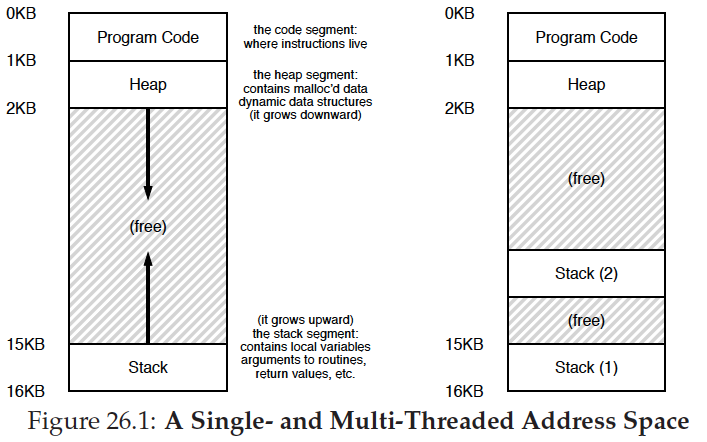
\includegraphics[width=0.75\textwidth]{fig/figure-26-1.png}
\caption{图26.1:单线程和多线程的地址空间} \label{fig:figure-26-1}
\end{figure}

然而,在多线程进程中,每个线程独立运行,当然会调用各种各样的routines来完成它正在做的任何工作。跟地址空间中只有一个栈不同,多线程进程中每个线程都有一个栈。假设一个多线程进程内有两个线程,其相应的地址空间与经典进程不一样(见上右图)。

在Figure26.1中,可以看到两个栈分布在进程的"整个"地址空间中。因此,任何在栈中分配的变量、参数、返回值以及其他存放在栈中的数据将会存储在那个有时称作线程局部空间的地方,即相应线程的栈。

也许你也注意到了新的布局破坏了原来"美观"的地址空间布局。之前,堆栈可以各自独立增长而不出问题,除非超出了地址空间的范围。而现在的地址空间布局就不再有先前的"nice situation"。幸运的是,这样的空间布局通常是可行的,因为栈一般不需要特别大(程序大量使用递归时除外)。

\section{例子:线程创建}
假设我们想运行一个创建两个线程的程序,每个线程各自执行相互独立的任务,打印「A」或「B」。代码如Figure 26.2所示。

主程序创建两个线程,每个都执行函数mythread(),但是传递不同的参数(字符串『A』或『B』)。一旦创建了线程,它可能会立即运行(取决于调度器的whims);也可能会进入『就绪』态而非『运行』态,因此不立即执行。创建两个线程之后(T1和T2),主线程调用pthread\_join()等待对应的线程结束。
\begin{figure}[t]
\begin{lstlisting}
#include <stdio.h>
#include <assert.h>
#include <pthread.h>

void *mythread(void *arg) {
    printf("%s\n", (char *) arg);
    return NULL;
}

int
main(int argc, char *argv[]) {
    pthread_t p1, p2;
    int rc;
    printf("main: begin\n");
    rc = pthread_create(&p1, NULL, mythread, "A"); assert(rc == 0);
    rc = pthread_create(&p2, NULL, mythread, "B"); assert(rc == 0);
    // join waits for the threads to finish
    rc = pthread_join(p1, NULL); assert(rc == 0);
    rc = pthread_join(p2, NULL); assert(rc == 0);
    printf("main: end\n");
    return 0;
}
\end{lstlisting}
\caption{简单的线程创建代码}
\end{figure}

我们来看一下这个小程序可能的执行顺序,在执行示意图中(表 26.1),时间从上向下依次增长,每一栏显示了什么时候运行不同的线程(主线程、线程T1、或线程T2)。

然而,注意这个顺序并不是唯一的执行顺序。实际上,对于一个给定的指令序列,它有不少的可能执行顺序,这取决于在特定的时刻调度器决定哪个线程能得到执行。比如,一旦创建了一个线程,它可能立即执行,如表26.2所示的执行顺序。

我们也可以看到『B』在『A』之前打印出来,这就是说调度器决定先执行线程T2,即使线程T1更早创建;没有任何理由取假设先创建的线程就先运行。表26.3显示了这个执行顺序,线程T2*******with Thread 2 getting to strut its stuff before Thread 1.

As you might be able to see, one way to think about thread creation is that it is a bit like making a function call; however, instead of first executing the function and then returning to the caller, the system instead creates a new thread of execution for the routine that is being called, and it runs independently of the caller, perhaps before returning from the create, but perhaps much later. 

As you also might be able to tell from this example, threads make life complicated: it is already hard to tell what will run when! Computers are hard enough to understand without concurrency. Unfortunately, with concurrency, it gets worse. Much worse.

\begin{table}[p]
\centering
{\scriptsize
\begin{tabular}{p{5cm} l l}
\textbf{main}&\textbf{Thread 1}&\textbf{Thread 2}\\ \midrule[1.1pt]
starts running &  & \\
prints "main:begin" &  & \\
creates Thread 1&  &  \\
creates Thread 2&  &  \\
waits for T1&  &  \\
  & runs &  \\
  & prints "A" &  \\
  & returns &  \\
waits for T2 &  &  \\
  &  & runs \\
  &  & prints "B" \\
  &  & returns \\
prints "main:end" &  &  \\
\end{tabular}}
\caption{\footnotesize 线程执行轨迹(1)}\color{black}\label{tab26-1}

\vspace{0.5cm}
{\scriptsize
\begin{tabular}{p{5cm} l l}
\textbf{main}&\textbf{Thread 1}&\textbf{Thread 2}\\ \midrule[1.1pt]
starts running &  & \\
prints "main:begin" &  & \\
creates Thread 1&  &  \\
  & runs &  \\
  & prints "A" &  \\
  & returns &  \\
creates Thread 2&  &  \\
  &  & runs \\
  &  & prints "B" \\
  &  & returns \\
waits for T1&  &  \\
\textsl{~~~~returns immediately; T1 is done} &  & \\
waits for T2 &  &  \\
\textsl{~~~~returns immediately; T2 is done} &  & \\
prints "main:end" &  &  \\
\end{tabular}}
\caption{{\footnotesize 线程执行轨迹(2)}}\color{black}\label{tab26-1}

\vspace{0.5cm}
{\scriptsize
\begin{tabular}{p{5cm} l l}
\textbf{main}&\textbf{Thread 1}&\textbf{Thread 2}\\ \midrule[1.1pt]
starts running &  & \\
prints "main:begin" &  & \\
creates Thread 1&  &  \\
creates Thread 2&  &  \\
  & runs &  \\
  & prints "A" &  \\
  & returns &  \\
waits for T1 &  &  \\
  &  & runs \\
  &  & prints "B" \\
  &  & returns \\
waits for T2 &  &  \\
\textsl{~~~~returns immediately; T2 is done} &  & \\
prints "main:end" &  &  \\
\end{tabular}}
\caption{\footnotesize 线程执行轨迹(3)}\color{black}\label{tab26-1}
\end{table}

\clearpage


\begin{lstlisting}
#include <stdio.h>
#include <pthread.h>
#include "mythreads.h"

static volatile int counter = 0;

/* Simply adds 1 to counter repeatedly, in a loop. No, this is not how 
 * you would add 10,000,000 to a counter, but it shows the problem nicely. */

void *mythread(void *arg) {
    printf("%s: begin\n", (char *) arg);
    int i;
    for (i = 0; i < 1e7; i++) {
        counter = counter + 1;
    }
    printf("%s: done\n", (char *) arg);
    return NULL;
}

/* Just launches two threads (pthread_create) and then waits for them (pthread_join) */

int main(int argc, char *argv[]) {
    pthread_t p1, p2;
    printf("main: begin (counter = %d)\n", counter);
    Pthread_create(&p1, NULL, mythread, "A");
    Pthread_create(&p2, NULL, mythread, "B");

    // join waits for the threads to finish
    Pthread_join(p1, NULL);
    Pthread_join(p2, NULL);
    printf("main: done with both (counter = %d)\n", counter);
    return 0;
}
\end{lstlisting}

%\begin{figure}[h]
%\caption{共享数据}
%\end{figure}

\section{为何更糟糕:共享数据}
上一节简单的线程示例可以有效的解释线程是如何被创建,以及它们是如何按照不同的顺序运行,这个执行顺序决定于调度器决定如何运行它们。这个示例并没有展示线程间在访问共享数据时是如何交互的。

让我们设想一个简单的例子:有两个线程想要更新一个全局共享变量。我们将要研究的代码见Figure 26.3。

有几个关于这段代码的注释。第一,如Stevens的建议【SR05】,我们封装了线程的create和join例程与其失败退出判断【***】,对于一个简单如此的程序,我们至少要关注发生的错误(如果发生的话),但是不做任何很【smart】的事儿(如:仅仅退出)。因,Pthread\_create()简单的调用pthread\_create()并确定返回值为0;如果不是,Pthread\_create()仅仅打印一个消息并退出。

第二,这个例子为工作线程仅用一个函数而不是两个独立的函数(即两个线程执行同一个函数,译者注),向线程传递一个参数(这里是字符串)让每一个线程在其消息之前打印不同的字母。

最后也是最重要的,我们可以看每个工作线程试图做的事:共享变量counter加1,这个操作在循环中执行一千万次。因此,理想的最终结果是:20,000,000。

现在编译执行这个程序,看一下它的结果。有时候,everything works how we might expect:
\begin{verbatim}
prompt> gcc -o main main.c -Wall -pthread
prompt> ./main
main: begin (counter = 0)
A: begin
B: begin
A: done
B: done
main: done with both (counter = 20000000)
\end{verbatim}

不幸的是,当我们运行这段代码时,即使是在一个处理器上,我们也得不到那个预期的结果。有时,结果如下:
\begin{verbatim}
prompt> ./main
main: begin (counter = 0)
A: begin
B: begin
A: done
B: done
main: done with both (counter = 19345221)
\end{verbatim}

我们再试一次,看看是不是我们疯狂了。毕竟,如你所接受的教育,计算机并不认为会产生确定性结果。也许你的处理器欺骗了你?(等我喘口气)
\begin{verbatim}
prompt> ./main
main: begin (counter = 0)
A: begin
B: begin
A: done
B: done
main: done with both (counter = 19221041)
\end{verbatim}

不仅每一个都是错误的结果,而且每个结果还不一样!大大的疑问:为什么会发生这样的事儿呢?

\begin{tcolorbox}[colframe=grey,colback= grey,arc=0pt,left=6pt,right=6pt,top=6pt,bottom=6pt,boxsep=0pt]
\begin{center}技巧:了解并使用你的工具
\end{center}

你总是需要学习心得工具来帮助你编写、调试和理解计算机系统。这里我们使用一个小巧的工具:反汇编器(disassembler)。当你对一个可执行文件执行反汇编时,它会显示这个可执行文件是有哪些会变代码组成的。例如,如果你希望理解例子中更新counter的底层代码,运行objdump(Linux)来它的汇编代码:
\begin{verbatim}
prompt> objdump -d main
\end{verbatim}
\end{tcolorbox}

\section{核心问题:失控的调度}
为了理解为何会发生这样的事儿,我们需要理解编译器为更新counter而生成的指令序列。在这个例子里,我们希望简简单单的将counter加1。因此,做这一操作的指令序列也许应该如下(x86):
\begin{verbatim}
mov 0x8049a1c, %eax
add $0x1, %eax
mov %eax, 0x8049a1c
\end{verbatim}

这个例子假设变量counter分配的地址是0x8049a1c。在这个三指令的序列里,x86的mov指令首先取得该地址的内存值并将其放入寄存器eax中,然后,执行add操作,eax寄存器的值加1,最后,eax的值写回原先的内存地址。

我们设想一下两个线程中的一个(线程T1)进入这段代码,它对counter执行了加1操作。它首先加载counter的值(假设其初值是50)进入寄存器eax,因此对线程T1来说寄存器eax的值为50。然后它对寄存器执行加1操作,此时eax的值是51。现在,发生了件不幸的事儿:定时器中断到达;因此,操作系统保存当前运行线程的状态(PC,eax等寄存器)至线程的TCB。

现在发生了更糟糕的事儿:线程T2被调度执行,它进入同一段代码。它也执行第一条指令,获取counter的值并写入它的eax寄存器(注:每个线程在运行时都有自己私有的寄存器;这些寄存器是通过上下文切换代码保存、加载虚拟化出来)。counter的值此时仍然是50,因此线程T2的eax值为50。假设线程T2继续执行接下来的两条指令,eax加1(eax=51),然后保存eax的内容至counter(内存地址0x8049a1c)。因此,全局变量counter此时的值是51。

最后,又一次发生上下文切换,并且线程T1得到了执行。记得刚才仅仅执行过了mov和add指令,那么此时应当执行最后一条mov指令。刚才eax的值是51,因此,最后执行mov指令并将值写入内存;counter的又一次被写为51。

简单的说,事儿是这样的:counter加1的代码执行了两次,但是初值为50的counter现在只有51。但是这个程序『正确的』结果应当是变量counter值为52。

我们来看一下详细的执行路径以便更好的理解这个问题。对于这个例子,假设上述的代码加载到内存地址100处,如下图所示的指令序列(注意那些曾经优秀的精简指令集:x86有变长指令;这里的mov指令占5字节的内存,add指令仅占3字节):
\begin{verbatim}
100 mov 0x8049a1c, %eax
105 add $0x1, %eax
108 mov %eax, 0x8049a1c
\end{verbatim}
基于这些假设,上述发生的事儿如表26.4所示。假设counter起始值是50,然后跟踪这个例子确保你可以理解正在发生什么。
\begin{table}[h]
{\footnotesize
\begin{tabular}{p{3cm} p{3cm} p{3cm} c c c}
 & & & \multicolumn{3}{c|}{after instruction} \\
\textbf{OS}&\textbf{Thread 1}&\textbf{Thread 2} & \textbf{PC}  & \textbf{\%eax} & \textbf{counter}\\
\midrule[1.1pt]
 & before critical section &  & 100 & 0 & 50 \\
 & mov 0x8049a1c, \%eax  &  & 105 & 50 & 50\\
 & add \$0x1, \%eax &  & 108 & 51 & 50 \\
 \textbf{interrupt} & & & & & \\
 ~~~~\textsl{save T1's state} & & & & & \\
 ~~~~\textsl{restore T2's state} & & & 100 & 0 & 50 \\
  & & mov 0x8049a1c, \%eax & 105 & 50 & 50 \\
  & & add \$0x1, \%eax & 108 & 51 & 50 \\
  & & mov \%eax, 0x8049a1c & 113 & 51 & 51 \\
\textbf{interrupt} & & & & & \\
 ~~~~\textsl{save T2's state} & & & & & \\
 ~~~~\textsl{restore T1's state} & & & 108 & 51 & 50 \\
  & mov \%eax, 0x8049a1c & & 113 & 51 & 51 \\
\end{tabular}}
\caption{问题:up close and personal}\color{black}\label{tab26-1}
\end{table}

上面已经示范的问题称作:竞争条件,其结果取决于这段代码的执行时机。有时候运气不好(例如:在执行的时候发生不合时宜的上下文切换),就会得到错误的结果。实际上,我们很可能每次都得到不同的值;因此,而不是确定性计算(曾经来源于计算机??),我们称之为不确定性,不知道输出的会是什么,且这些输出在交叉运行之间很可能会不同。

因为多线程执行这段代码会引起竞争条件,我们称这段代码为:临界区。一个临界区是一段访问共享变量(更一般的;共享资源)且不可被多于一个线程并发执行的代码段。

对于这段代码,我们需要的是称之为互斥量的东西。这个性质保证了如果有一个线程正在执行临界区代码,其他的线程都会被阻止进入临界区。

顺便提一下,实际上所有这些概念都是由Edsger Dijkstra创造出来的。他是这个领域的开拓者,并凭借这个工作和其他成果获得了图灵奖;详见他1968年的论文『Cooperating Sequential Processes』[D68]中对此问题惊人清晰的描述。我们还会在本章中多次看见Dijkstra。

\section{原子性的愿望}
解决这个问题的一个办
法是更强大的指令,这些指令可以在单步之内做任何我们需要做的,因此避免了发生不合时宜的中断的可能性。例如,假如我们有一个像下面所示一样的超级指令,会怎样呢?
\begin{verbatim}
memory-add 0x8049a1c, $0x1
\end{verbatim}

假设这条指令将一个值加到该内存地址,并硬件保证它是原子执行的;当这条指令执行后,它将按照预想的那样执行更新操作。它不会在指令执行中被中断,因为正是我们从硬件那儿得到的保证:当中断发生时,这条指令要么没有执行,要么已经执行结束;没有中间状态。硬件可以如此的美好,不是么?

在此文中,原子性意味着『作为一个单位』,有时称之为『全或无』。我们想原子地执行这三条指令序列:
\begin{verbatim}
mov 0x8049a1c, %eax
add $0x1, %eax
mov %eax, 0x8049a1c
\end{verbatim}

如之前所说的,如果有一条单独指令能够完成这个操作,那么只需要发出指令即可完成。但是通常情况下,没有这样的指令。设想我们已经构建了一个并发的B树,此时想要更新它;难道要硬件支持『B树的原子更新』指令么?恐怕不可能,至少在合理的指令集中是如此。

因此,相反的,由硬件提供少量有效的指令,我们可以借助这些指令构建一系列通用的同步原语。通过这些硬件同步原语与操作系统的支持,我们可以构造出以同步可控方式访问临界区的多线程代码,因此可以可靠的生成正确的结果,尽管存在并发执行的挑战。相当的棒,是不?

这是本节将要研究的问题。这是一个奇妙也很难的问题,应该会让你(有点)头疼。如果没有头疼,那就是你没懂!继续研究直到你头疼为止,那时候你就知道自己已经走向了正确的方向。到了那个时候,休息一会儿,我们可不想让你头疼的厉害。
\begin{tcolorbox}[colframe=grey,colback= grey,arc=0pt,left=6pt,right=6pt,top=6pt,bottom=6pt,boxsep=0pt]
\begin{center}症结所在:如何为同步提供支持\end{center}

为了构建有效的同步原语,我恩需要硬件提供什么支持呢?又需要操作系统提供什么支持呢?我们怎么才能正确高效的构建这些原语呢?程序又如何使用他们以得到期望的结果呢?
\end{tcolorbox}

\begin{tcolorbox}[colframe=grey,colback= grey,arc=0pt,left=6pt,right=6pt,top=6pt,bottom=6pt,boxsep=0pt]
\begin{center}
关键并发术语\\
临界区,竞争条件,不确定性,互斥
\end{center}
这四个术语对于并发代码太核心了,以至于我认为非常值得把它们提出来说一下。详见Dijkstra早期的工作[D65,D68]。
\begin{itemize}
\item 临界区,临界区是一段访问共享资源的代码段,共享资源一般是一个变量或数据结构
\item 竞争条件,竞争条件发生在正在执行的多个线程几乎同时进入临界区;多个线程都试图更新共享数据结构,同时导致产生奇怪(可能非预期)的结果。
\item 不确定性,一段不确定的程序有一个或多个竞争条件组成,一次一次执行的输出变化不一,视不同线程何时运行而定。因此结果是不确定的,通常我们指望着计算机系统。
\item 互斥,为了避免这个这些问题,线程需要使用某种互斥原语;以此保证只有一个线程已经进入临界区,从而避免竞争得到确定性的结果。
\end{itemize}
\end{tcolorbox}

\section{另一个问题:等待其他线程}
本章所设定的并发问题,线程间貌似只有一种交互形式,即访问共享变量以及临界区原子性的支持。事实证明,还会产生另一种常见的交互,即一个线程必须等待其他线程完成某些操作方能继续执行。例如,当一个进程执行磁盘I/O时而休眠时,这种交互就会产生;当磁盘I/O完成时,进程需要从休眠中唤醒以便继续执行。
因此,在接下来的章节中,我们不仅仅会研究如何构建同步原语为原子性提供支持,还会研究相应的机制来为多线程程序中常见的休眠唤醒交互方式提供支持。
要是现在这东西没有意义,那好!当你读到条件变量那章时就会觉得有意义了。如果那时觉得不太行,那你应该一遍再一遍的读那章直到觉得有意义。

\section{小结:为什么在OS级}
在wrapping up之前,你可能有一个疑问:为什么我们要在OS这一层研究这些?答案就一个词——历史;操作系统是第一个并发程序,许多技术都被创造用于OS中。后来,在多线程进程中,应用程序编写者也不得不考虑这些事儿。

例如,设想这样的场景,有两个正在运行的进程。假如它们都调用write()来写一个文件,都想将数据附加到文件中(例如:添加数据到文件末尾,从而增加它的长度)。这样的话,两者都需要分配一个新的块,记录块的位置到文件的inode中,并改变文件大小以示一个更大的大小(我们将会在本书第三部分学到更多关于文件的内容)。因为中断可能随时都会发生,更新这些共享数据结构的代码就是临界区,因此,从最开始的中断介绍可知,操作系统设计者不得不担心操作系统怎么更新这些内部结构。一个不合时宜的中断引起了上述的所有问题。不奇怪,页表,进程列表,文件系统结构等。实际上,所有内核数据结构都需要通过合适的同步原语来谨慎访问,以便正确工作。

\begin{tcolorbox}[colframe=grey,colback= grey,arc=0pt,left=6pt,right=6pt,top=6pt,bottom=6pt,boxsep=0pt]
\begin{center}技巧:使用原子操作\end{center}
原子操作是构建计算机系统最强大的底层技术之一,从计算机体系结构到并发代码(本节正在研究的)、文件系统(后面将会研究的)、数据库管理系统,甚至分布式系统[L+93]。
使得一系列行为原子化背后的思想可以简单的缩成一个短语——全或无。你希望一起执行的行为要么全都发生了,要么全都没有发生,而没有中间状态。有时,将许多行为组织成一个原子行为称作:事务,这个思想在数据库和事务处理领域已经发展很成熟[GR92]。
在探索并发性的主题中,我们会使用同步原语把短指令序列转化成原子执行块。但是如我们将会见到的,原子性的思想远不止这些。例如,文件系统使用诸如日志或copy-on-write等技术来原子地转移它们的磁盘状态,使得在面对系统故障时能严格正确地执行。If that doesn’t make sense, don’t worry—it will, in some future chapter。
\end{tcolorbox}



\chapter{插曲:线程API}
\thispagestyle{empty}

本章简要讲解线程API的主要内容。每个部分将会按照介绍如何使用这些API的顺序,在后续章节进行详细解释。更多的细节可以在许多书和在线资源里找到[B97,B+96,K+96]。需要注意,由于有很多的例子,接下来锁和条件变量概念的章节讲起来会很慢;因此,本章用作一个引用会更好些。

\begin{tcolorbox}[colframe=grey,colback= grey,arc=0pt,left=6pt,right=6pt,top=6pt,bottom=6pt,boxsep=0pt]
\begin{center}关键:如何创建并控制线程
\end{center}
操作系统应该为线程创建和控制提供什么接口?应该如何设计这些接口,使之跟一般程序接口一样使用自如?
\end{tcolorbox}

\section{线程创建}
编写多线程程序,首先要做的就是创建新线程;因此,需要存在某种线程创建接口。在POSIX中,很简单:
\begin{verbatim}
#include <pthread.h>
int  pthread_create( pthread_t * thread,  const pthread_attr_t * attr,
                     void * (*start_routine)(void*),  void * arg);
\end{verbatim}
这个声明貌似有点小复杂(特别是当你没有用过C语言的函数指针),其实这并不糟糕。这里有四个参数:thread,attr,start\_routine,arg。第一个参数thread是一个指向pthread\_t结构体的指针;我们将会用这个结构体与起对应的线程进行交互,因此我们需要将它传给pthread\_create()函数初始化。

第二个参数attr,用来指定一些这个线程可能需要的一些属性。比如设置栈大小,或者这个线程的调度优先级的信息等。可以单独调用pthread\_attr\_init()函数来初始化一个属性;欲知详情,请查阅对应手册。然而,许多情况下,默认属性就可以了,这样的话,给该参数传递一个NULL即可。

第三个参数是最复杂的,实际上它只是想知道:这个线程从哪个函数开始运行?在C语言中,称之为函数指针。这个函数指针告诉我们一下信息:函数名(start\_routine),传递给该函数一个void *类型的参数(如start\_routine括号之后表示的),以及该函数一个类型为void *的返回值(例如:空指针)。

如果这个函数指针想要的不是空指针,而是一个整型参数,其声明如下:
\begin{verbatim}
int pthread_create(..., // 前两个参数一样
                    void * (*start_routine)(int), int arg);
\end{verbatim}
如果函数指针希望传一个空指针参数,但是要返回一个整型值,则其声明如下:
\begin{verbatim}
int pthread_create(..., // 前两个参数一样
                    int (*start_routine)(void *), void * arg);
\end{verbatim}

最后,第四个参数arg实际上就是传递个函数指针的参数。你可能会有疑问:为什么需要这些空指针呢?其实答案很简单:start\_routine函数有了一个空指针作为参数,就可以传递任意类型的参数给它了;有一个空指针的返回值就允许线程返回任意类型的结果。
\begin{figure}[h]
\begin{lstlisting}
#include <pthread.h>

typedef struct __myarg_t {
	int a;
	int b;
}myarg_t;

void *mythread(void *arg) {
	myarg_t *m = (myarg_t *) arg;
	printf("%d %d\n", m->a, m->b);
	return NULL; 
}

int main(int argc, char *argv[]) {
	pthread_t p;
	int rc;
	myarg_t args;
	args.a = 10;
	args.b = 20;
	rc = pthread_create(&p, NULL, mythread, &args);
	...
}
\end{lstlisting}
\caption{创建线程}
\end{figure}

我们来看图27.1的例子。仅创建了一个传递了两个参数的线程,这两个参数组成自己定义的类型(myarg\_t)。一旦创建后,这个线程就可以简单地将它的参数转化成想要的类型,并可按预期得到这些参数。

一旦创建了线程,就会存在一个新的存活的执行实体,与它自己的调用栈一起完成,跟程序中所有存在的线程一样运行在相同的地址空间。快乐之旅由此开始!

\begin{lstlisting}
#include <stdio.h>
#include <pthread.h>
#include <assert.h>
#include <stdlib.h>

typedef struct __myarg_t {
	int a;
	int b;
} myarg_t;
typedef struct __myret_t {
	int x;
	int y;
} myret_t;

void *mythread(void *arg) {
	myarg_t *m = (myarg_t *) arg;
	printf("%d %d\n", m->a, m->b);
	myret_t *r = Malloc(sizeof(myret_t));
	r->x = 1;
	r->y = 2;
	return (void *) r;
}

int main(int argc, char *argv[]) {
	int rc;
	pthread_t p;
	myret_t *m;

	myarg_t args;
	args.a = 10;
	args.b = 20;
	Pthread_create(&p, NULL, mythread, &args);
	Pthread_join(p, (void **) &m);
	printf("returned %d %d\n", m->x, m->y);
	return 0;
}
\end{lstlisting}
\begin{figure}[h]
\setlength{\abovecaptionskip}{1pt}
\caption{等待线程完成}
\setlength{\belowcaptionskip}{1pt}
\end{figure}

\section{线程完成(completion)}
之前的例子展示了如何创建一个线程。然而,如果想要等待一个线程的完成会发生什么呢?你需要做一些特别的事儿来等待线程完成;特别的,你需要调用的pthread\_join()函数。
\begin{verbatim}
int pthread_join(pthread_t thread, void **value_ptr);
\end{verbatim}
这个函数只有两个参数,第一个参数是pthread\_t类型,用来指定要等待哪个线程。实际上就是在创建线程时传递给线程库的那个值;如果持有这个值,那么现在就可以用来等待那个线程的运行终止。

第二个参数是一个指向你想要取回的返回值的指针。因为这个函数可以返回任意值,故其定义成了一个空指针;由于pthread\_join会改变传给它的参数,故应该传递该值的指针,而不是值本身。

我们来看另外一个例子(图27.2)。在这段代码里,还是创建了一个线程,并通过myarg\_t结构体传递了一对参数。返回值用到了myret\_t类型。一旦这个线程结束运行,正等在pthread\_join()的主线程就会返回,并且可以访问从线程返回的值,即myret\_t里的内容。



这个例子有几个注意点。第一,大多数时候我们不需要做所有这些痛苦的 packing and unpacking of arguments的事儿。例如,如果我们仅需创建一个无参的线程,传递一个NULL作为参数即可。类似的,如果我们不关心返回值的话,可以给pthread\_join()传一个NULL。
第二,如果我们仅传一个值的话(如int),就不需要package它作为一个参数。图27.3就是一个例子。这种情况下,由于我们不需要将参数和返回值package成结构体,就简单了很多。

\begin{figure}[h]
\begin{lstlisting}
void *mythread(void *arg) {
	int m = (int) arg;
	printf("%d\n", m);
	return (void *) (arg + 1);
}

int main(int argc, char *argv[]) {
	pthread_t p;
	int rc, m;
	Pthread_create(&p, NULL, mythread, (void *) 100);
	Pthread_join(p, (void **) &m);
	printf("returned %d\n", m);
	return 0;
}
\end{lstlisting}
%\setlength{\abovecaptionskip}{2pt}
\caption{等待线程完成}
\end{figure}

第三,需要非常注意返回值是如何从线程返回的。尤其,不要返回一个指向了线程调用栈中分配的值的指针。如果这么做了,你觉得会发生什么呢?(考虑一下)这里是一段问题代码的例子,改自图27.2中的例子。

\begin{verbatim}
void *mythread(void *arg) {
    myarg_t *m = (myarg_t *) arg;
    printf("%d %d\n", m->a, m->b);
    myret_t r; // 分配在栈中: BAD!
    r.x = 1;
    r.y = 2;
    return (void *) &r;
}
\end{verbatim}

在这种情况下,变量r是在mythread的栈中分配的。然而,当线程返回时,这个值会自动释放(这就是为什么栈使用起来这么简单)。因此,传回去的指针就是一个未分配的变量,可能会导致各种错误结果。当然,当你输出你觉得你返回了的值时,你很可能(不一定)会感到奇怪。可以自己试试看!【2. 幸运的是当你这样的代码时,编译器gcc可能会抱怨的,这也是一个注意编译器警告的原因】

最后,你可能注意到使用pthread\_create()创建线程之后,紧接着就调用了pthread\_join(),这种创建线程的方式很奇怪。实际上,有一种更容易的方式来完成这样的任务,叫做过程调用。通常我们会创建不止一个线程并等待它完成,否则完全没有使用多线程的意义。

我们应该注意到并不是所有的多线程代码都使用join函数。例如,一个多线程web服务器可能创建多个工作线程(worker),然后使用主线程accept请求并将之传给工作线程(worker)。因此,这样长生存期的程序也许就不需要join。然而,一个创建多个线程去并行执行特定任务并行程序很可能会用join来确保所有的工作都完成,才退出或进入下一阶段工作。

\section{锁}
除了线程创建(creation)和合并(join),也许,POSIX线程库提供的最有用的一些列函数是通过锁(locks)来为临界区提供互斥量的函数。这对最基础的函数由下列两个函数提供:
\begin{verbatim}
int pthread_mutex_lock(pthread_mutex_t *mutex);
int pthread_mutex_unlock(pthread_mutex_t *mutex);
\end{verbatim}

这两个函数应该很容易理解和使用。当你实现的一段代码是临界区时,需要用锁来保护以使按照预期执行。你大概可以想象一下,代码应该如下:
\begin{verbatim}
pthread_mutex_t lock;
pthread_mutex_lock(&lock);
x = x + 1; // or whatever your critical section is
pthread_mutex_unlock(&lock);
\end{verbatim}

这段代码的意思是这样的:如果在调用pthread\_mutex\_lock()时没有其他的线程持有这个锁,这个线程就取获取这个锁,并进入临界区。如果其他线程已经持有这个锁,则这个试图获取锁的线程会阻塞直到获取到锁(意味着那个持有锁的线程已经调用unlock释放了这个锁)。当然,有可能在一个给定的时间会有很多线程卡在线程获取函数;只有那个获取到锁的调用unlock。【*****】

可惜,这段代码在两个地方有问题。第一个问题是:未有合适的初始化。所有的锁都必须被正确地初始化,以保证它们都有正确的初始值,以及在调用lock和unlock时能够正常工作。

在POSIX线程中,有两种初始化锁的方式。一种是用 PTHREAD\_MUTEX\_INITIALIZER来初始化,如下:
\begin{verbatim}
pthread_mutex_t lock = PTHREAD_MUTEX_INITIALIZER;
\end{verbatim}

这种方式将锁设置为默认值并设为可用。另一种动态方式是调用 pthread\_mutex\_init(),如下:
\begin{verbatim}
int rc = pthread_mutex_init(&lock, NULL);
assert(rc == 0); // always check success!
\end{verbatim}

第一个参数是锁的地址,而第二个参数是一个可选的属性集。关于该属性集可以自己查阅;简单地传递NULL则是使用默认方式。上述的两种方式都可以,但我们通常使用动态的方法(后者)。注意,当锁使用结束时,相应的要调用 pthread\_mutex\_destroy()。可参见相应的手册获取这部分的所有细节。

第二个问题是没有检测lock和unlock调用的错误码。就像你在UNIX系统中调用几乎所有的库函数一样,这些函数也可能失败!如果你的代码没有正确的检测错误码,那么错误就会默默的发生,这种情况下就有可能多个线程都进入了临界区。最起码,要用断言将其封装(如图27.4);更多的成熟(non-toy)的程序,在出错时不能简单的退出,当lock和unlock失败时,应当检测错误并采取一些适当措施。

\begin{figure}[h]
\begin{verbatim}
// Use this to keep your code clean but check for failures
// Only use if exiting program is OK upon failure
void Pthread_mutex_lock(pthread_mutex_t *mutex) {
    int rc = pthread_mutex_lock(mutex);
    assert(rc == 0);
}
\end{verbatim}
\setlength{\abovecaptionskip}{2pt}
\caption{简单封装}
\end{figure}

lock和unlock函数并不是pthreads仅有的锁相关函数。特别的,还有两个函数可能感兴趣函数:
\begin{verbatim}
int pthread_mutex_trylock(pthread_mutex_t *mutex);
int pthread_mutex_timedlock(pthread_mutex_t *mutex,
                            struct timespec *abs_timeout);
\end{verbatim}
这两个函数在获取锁时使用。trylock函数会在锁已经被持有时返回失败;timedlock函数会在得到了锁或者超时之后返回,无论那个先发生。因此,timedlock函数在超时值为0时退化成trylock函数。一般讲,要避免使用这两个函数;然而,有少部分时候为了避免阻塞在获取锁上,这两函数还是很有用的,正如下一章我们将讲到的(如:当我们研究死锁时)。

\section{条件变量}
线程库的另一个主要组件就是条件变量,当然POSIX线程也是这样。当某种信号必须在信号间发生时,条件变量是很有用的,如一个线程需要等待其他线程完成某事才能继续执行。程序希望以这种方式交互时,会常用两个函数:
\begin{verbatim}
int pthread_cond_wait(pthread_cond_t *cond, pthread_mutex_t *mutex);
int pthread_cond_signal(pthread_cond_t *cond);
\end{verbatim}

要使用条件变量,另外还需要有一个与之关联的锁。当调用这两个函数时,都要先持有对应的锁。

第一个函数,pthread\_cond\_wait(),会使调用线程休眠,等待其他线程唤醒它,通常是这个休眠的线程关心的某些事发生了改变。例如,典型的使用如下:
\begin{verbatim}
pthread_mutex_t lock = PTHREAD_MUTEX_INITIALIZER;
pthread_cond_t init = PTHREAD_COND_INITIALIZER;
Pthread_mutex_lock(&lock);
while (initialized == 0)
     Pthread_cond_wait(&init, &lock);
Pthread_mutex_unlock(&lock);
\end{verbatim}

这段代码,在初始化了相关的锁和条件变量之后,线程检测变量initialized是否已经被设置为其他值而非0。如果没有,线程就简单的调用wait函数休眠,直到其他线程唤醒它。

其他线程中唤醒这个线程的代码如下:
\begin{verbatim}
Pthread_mutex_lock(&lock);
initialized = 1;
Pthread_cond_signal(&init);
Pthread_mutex_unlock(&lock);
\end{verbatim}

这段代码的顺序有几点要注意。首先,当发送信号时(同样在修改全局变量initialized时),总是要确保已经持有了锁。这保证了我们不会在代码中引入竞争条件。

第二,你也许注意到了wait函数用了一个锁作为其第二的参数,而signal函数仅仅只有一个条件变量参数。造成这点不同的原因是,wait函数会将线程休眠,而wait函数需要在线程休眠前释放这个锁。设想一下如果不这么做:其他线程怎么获得这个锁并通知这个线程并唤醒呢?然而,在被唤醒之后,函数返回之前,pthread\_cond\_wait()函数会重新获取这个锁,因此确保了任何时间,等待线程是运行在持有锁和释放锁之间的。

最后一个奇怪的是,等待线程在while循环里重复检测了这个条件,而不是一个简单的if判断语句。在后面研究条件变量的章节中会详细讨论这个问题,【这里简单的说】,一般的,用while循环是简单并安全的。虽然它重复检测这个条件(也许会增加一些负载),但是有一些pthread实现可能会虚假的唤醒等待线程;这种状况下,不重复检测的话,等待线程就会认为条件已经改变了,而实际上却没有改变。因此,将唤醒视作等待条件可能已经修改的提示而不是视作一个绝对的事实,这样会更安全一些。

注意到有时候,用一个简单的flag标志在两个线程间传递信号,而不用条件变量及其关联的锁,这是很诱人的。例如,我们可以将上面的等待代码改写成这样:
\begin{verbatim}
while (initialized == 0)
; // 空转
\end{verbatim}

对应的发信号的代码像这样:
\begin{verbatim}
initialized = 1;
\end{verbatim}

千万不要这么做,有以下几个原因。第一,许多情况下,它的性能很差(长时间空转只是在浪费CPU时间)。第二,它很容易出错。如最近的研究表明[X+10],像上述那样在线程间使用flag标志同步,是极其容易出错的;粗略的说,使用这种临时同步方法的代码,半数都是有bug的。别偷懒,乖乖的用条件变量,即使你觉得你可以避免这个问题。

\section{编译运行}
本章所有的示例代码都是比较容易上手并运行的。要编译这些代码的话,必须包含pthread.h头文件。在链接的时候,必须加上-pthread来显示的链接线程库。
例如,要编一个简答的多线程程序,需要做的如下:
\begin{verbatim}
prompt> gcc -o main main.c -Wall -pthread
\end{verbatim}

只要在main.c中包含了pthreads线程库的头文件,你就可以成功的编译并发程序了。这个程序能否如预期执行就是另一码事。

\section{小结}
本章介绍了线程库的基础内容:线程创建,通过锁创建互斥量,以及通过条件变量发信号和等待。除了耐心跟细心,不再需要其他东西就可以写出健壮高效的多线程程序。

我们以一些tips结束本章,这些tips可能在你编写多线程代码时很有用(详见下一页的aside)。本章提到的API还有其他一些有意思的方面,如果你想获得更多信息,可以在Linux终端里输入man -k pthread来查看整个接口的一百多个API。然而,本章讨论的基础应该可以让你构建出优秀(也希望正确且高性能)的多线程程序。多线程最困难的不是这些API,而是你如何构建并发程序的复杂逻辑。继续阅读学习更多内容。

\begin{tcolorbox}[colframe=grey,colback= grey,arc=0pt,left=6pt,right=6pt,top=6pt,bottom=6pt,boxsep=0pt]
\begin{center}Aside:线程API指南
\end{center}
当你使用POSIX线程库构建一个多线程程序时,有一些细小但却很重要的注意点需要记住。他们是:

\begin{itemize}
\item \textbf{保持简单}。这一点高于一切,任何在线程间加锁或发信号的代码都要尽可能的简单。复杂的线程交互可能会导致bug。
\item \textbf{最小化线程交互}。保持线程间交互的方式最小。每一次交互都要仔细考虑,并通过尝试和正确的方法来构造(这些方法会在接下来的章节中学习)。

\item \textbf{初始化锁和条件变量}。不这么做的话,你的代码就会很奇怪,有时候好好的,有时候就出错。

\item \textbf{检查返回码}。当然,在你编写的任何C和UNIX程序,都应该检查每一个返回码,这一点在并发程序中也适用。不这么做的话,可能会导致奇怪的很难理解的行为,很可能会使你要么抓狂,要么扯头发【很可能会使你抓狂】。

\item \textbf{注意如何传参给线程},如何从线程返回值。特别的,传递一个在栈中分配的变量的引用的话,很有可能你就错了。

\item \textbf{每个线程都有自己的栈}。跟前一点相关的,记住每个线程都有自己的栈空间。因此,如果某个线程在执行某个函数的时候,有一个局部分配的变量,这个变量本质上是该线程私有的;任何其他线程都没法轻易的访问它。要想在线程间共享数据,该变量应当在堆(heap)中或某个全局可访问的地方。

\item \textbf{永远使用条件变量在线程间传信号}。使用简单的flag标志通常是很诱人的,但是不要这么做。

\item \textbf{使用手册页}。特别的,Linux的pthread手册页提供了非常有用的信息并讨论了许多本章提到的细微差别,而且更加详细。仔细阅读这些手册!
\end{itemize}
\end{tcolorbox}

\newpage

参考文献\\

[B97] “Programming with POSIX Threads”\\
David R. Butenhof\\
Addison-Wesley,May 1997\\
另一本关于线程的书。\\


[B+96] “PThreads Programming:\\
A POSIX Standard for Better Multiprocessing”\\
Dick Buttlar, Jacqueline Farrell, Bradford Nichols\\
O’Reilly, September 1996\\
O’Reilly家的一本不错的书。O’Reilly是一家非常优秀且很实用的一家出版社,我们的书架有很多这家公司的书,包括一些关于Perl、Python和Javascript的非常好的作品(尤其是Crockford的《Javascript: The Good Parts》)。\\


[K+96] “Programming With Threads”\\
Steve Kleiman, Devang Shah, Bart Smaalders\\
Prentice Hall, January 1996\\
本领域一本更好的书。值得收藏一本。\\


[X+10] “Ad Hoc Synchronization Considered Harmful”\\
Weiwei Xiong, Soyeon Park, Jiaqi Zhang, Yuanyuan Zhou, ZhiqiangMa\\
OSDI 2010, Vancouver, Canada\\
这篇文章展示了看似简单的同步代码是如何导致大量奇怪的bug的。用条件变量并正确的传递信号!

















\chapter{锁}
\thispagestyle{empty}

在并发性简介中,我们看到并发编程的一个基本问题:我们想要原子地执行一些列的指令,但是由于单处理器上中断的存在(或者多处理器上多线程并发执行),所以做不到。本章,我们通过提到过的锁来直接解决这个问题。程序员用锁标注源代码,将这些锁放在临界区的周围,因此确保这样的临界区像单条原子指令一样执行。

\section{基本思想}
作为示例,假设我们的临界区如下面的代码,一个典型的共享变量的更新:
\begin{verbatim}
balance = balance + 1;
\end{verbatim}
当然,也有可能是其他的临界区,比如把一个元素添加到链表中或者其他更复杂的共享数据结构的更新,但是这里我们仅仅用这个简单的例子。为了使用锁,在临界区的周围添加一些代码,如下:
\begin{verbatim}
1 lock_t mutex; // some globally-allocated lock ’mutex’
2 ...
3 lock(&mutex);
4 balance = balance + 1;
5 unlock(&mutex);
\end{verbatim}

锁只是一个变量,因此要使用锁的话,必须先声明一个某种类型的锁变量(比如上面的互斥量)。这个锁变量(简称锁)在任何时刻都持有这个锁的状态。它要么是可用的状态,因此没有线程持有这个锁;要么是已获取状态,因此恰有一个线程持有了这个锁,且可能进入了临界区。我们也可以在这个数据类型里存储一些其他信息,比如哪个线程持有了这个锁,或者等待获取锁的队列,但是这些信息是锁用户不可见的。

lock()和unlock()函数的语义很简单。调用函数lock()尝试获取这个锁;如果没有其他线程持有这个锁,这个线程就会获得这个锁并进入临界区;那么这个线程现在就是这个锁的拥有者。如果这时有其他线程对相同的锁变量(本例中的mutex)调用lock()函数,直到它持有这个锁之后才会返回;通过这种方式,就可以防止其他线程在第一个持有锁的线程进入临界区的时候也进入临界区。

一旦锁的拥有者调用了unlock(),锁就会又处于可获取状态(空闲)。如果没有其他线程等待这个锁(比如没有其他线程调用了lock()且阻塞在那里),那这个锁的状态就简单的转换称空闲态。如果有多个等待着的线程(阻塞在lock()函数), 其中一个线程会注意到(或者被通知)锁的状态变化,然后获得锁并进入临界区。

锁为程序员提供了最起码的调度控制。一般讲,我将线程视作有程序员创建但由操作系统调度的实体,不管操作系统选择以何种方式实现。锁将一部分线程调度控制权交还给了程序员;通过在临界区周围放置锁,程序员可以保证不会超过一个线程能进入该临界区。因此,锁将传统操作系统调度的混乱转变得更加可控了。


\section{线程锁}
POSIX库使用的锁的名字叫做mutex,因为它用于在线程间提供互斥量( mutual exclusion),例如,如果一个线程已经进入临界区了,这个线程就会排斥其他线程进来,直到自己执行完临界区的代码。因此,当你看到下面的POSIX线程代码时,你应该能够理解他实际上做的就是上面说的那些(还是使用检测了lock和unlock错误的封装函数):
\begin{verbatim}
pthread_mutex_t lock = PTHREAD_MUTEX_INITIALIZER;

Pthread_mutex_lock(&lock); // wrapper for pthread_mutex_lock()
balance = balance + 1;
Pthread_mutex_unlock(&lock);
\end{verbatim}

也许你还注意到POSIX版本的锁会想lock和unlock传一个变量,是因为我们可能要使用不同的锁来保护不同的变量。这样做可以提高并发性:用不同的锁保护不通的数据和数据结构,这就允许更多的线程马上进入锁住的代码(细粒度的方式),而不是一个任何时候任何临界区都可用的大锁(粗粒度的锁策略)。


\section{构造锁}
到现在为止,从程序员的角度,你应该对锁是如何工作的有了一些理解。但是我们如何构造一个锁呢?硬件需要提供什么支持呢?操作系统又需要支持什么呢?这些问题就是本章剩下的内容要讲的。

\begin{tcolorbox}[colframe=grey,colback= grey,arc=0pt,left=6pt,right=6pt,top=6pt,bottom=6pt,boxsep=0pt]
\begin{center}Crux:如何构造锁\end{center}
我们如何构造一个高效的锁?高效的锁以低开销提供了互斥量,同时也获得了一些其他性质,我们将在后面讨论。硬件需要提供什么支持呢?操作系统需要提供什么支持呢?
\end{tcolorbox}

要构造一个可用的锁,需要我们的朋友——硬件和操作系统提供一些帮助。多年来,个中计算机体结构的指令集都添加了许多不同的硬件原语;虽然我们不需要学习这些指令是如何实现的(毕竟这是计算机体系结构课上的话题),但是我们还是要学习如何使用这些指令来构造一个像锁一样的互斥量原语。我们还会研究操作系统是如何参与完成这个工作的,并帮助我们构建一个精密的锁库。


\section{评估锁}
在构造锁之前,我们应该首先要明白我们的目标是什么,并因此问自己如何评价某个特定锁实现的的效率。要评估一个锁是否有用,应该建立一些基础标准。第一点是,锁能够实现基本的任务,即提供互斥量。基本地,这个锁有效么,能够阻止多线程进入同一个临界区么?

第二点是公平。一旦锁空闲了,是否每个竞争该锁的线程都被公平对待?从另一个方式看的话,就是测试更极端的情况:是否有竞争该锁的线程处于饥饿状态而一直得不到锁?

最后一点就是性能,尤其是用锁后的增加的时间开销。这里有几个不同的情况值得考虑一下。一个是没有竞争的情况;当只有一个线程在运行、获取、释放锁,锁开销有多少?另一个是多线程在单CPU上竞争同一个锁的情况,是否需要担心其性能?最后一点,当引入多CPU,各个CPU上的多个线程竞争同一个锁的性能如何?通过对比这些不同的场景,我可以更好的理解使用各种锁技术对性能的影响。

\section{中断控制}
最早的互斥量的一个解决方案是为临界区关中断;这种方法是为单处理器系统设计的。其代码类似于下面:
\begin{verbatim}
void lock() {
     DisableInterrupts();
}
void unlock() {
     EnableInterrupts();
}
\end{verbatim}

假设程序运行在一个单处理器系统上。通过在进入临界区前关中断(用某种特殊的硬件指令),我们可以确保进入了临界区的代码不会被中断,因此就可以好像原子一样的执行。临界区代码执行结束后重新开中断(还是用硬件指令),因此程序就可以像平常一样继续。

这个方法的好处就是简单。你当然不用想破了脑子去弄明白为什么这方法是可行的。没有了中断,线程就可以保证它执行的代码确实会执行,并且不会有其他线程会干扰它。

可是,负面影响有很多。首先,这个方法要求我们允许任何调用线程取执行特权操作(即中断的开和关),而且还要信任这个功能不会被滥用。正如你知的,任何时候我都要信任随意一个程序,很有可能会有麻烦的。麻烦会以多种方式发生:一个贪心的程序可能在一开始的时候调用lock(),因此而独占处理器;更糟糕的,一个不当的或者恶意的程序可能会调用lock()并进入无限循环。在后一种情况下,操作系统不能重新获得系统的控制权,只有一种办法:重启系统。用关中断作为一种通用的同步方案要求对应用程序太多的信任。

第二,这种方法在多处理器上行不通。如果多个线程运行在多个不同的CPU上,每个线程都试图进入相同的临界区,无论中断是否已经关了,线程还可以运行在其他的处理器上,并因此而进入了临界区。由于多处理器现在很普遍了,我们的通用方案必须要比这个方案好。

\begin{tcolorbox}[colframe=grey,colback= grey,arc=0pt,left=6pt,right=6pt,top=6pt,bottom=6pt,boxsep=0pt]
\begin{center}Aside:Dekker和Peterson的算法\end{center}
在二十世纪六十年代,Dijkstra跟自己的朋友们提出了一个并发性问题,而且其中的一位叫做Theodorus Jozef Dekker的数学家提出了一个解决方案[D68],不像我们这个讨论的方案——用特殊的硬件指令,甚至是操作系统的支持,Dekker的算法仅仅使用load和store(假设它们彼此间是原子的,这在早期的硬件确实是的)。

Dekker的方法后来被Peterson改进了[P81]。这次也仅仅只用了load和store,它的思想是确保两个线程从不会同时进入一个临界区。下面是Peterson的算法(对于两个线程);如果能理解的话,可以看看。flag和turn变量用来做什么呢?
\begin{verbatim}
int flag[2];
int turn;
void init() {
     flag[0] = flag[1] = 0; // 1->thread wants to grab lock
     turn = 0; // whose turn? (thread 0 or 1?)
}
void lock() {
     flag[self] = 1; // self: thread ID of caller
     turn = 1 - self; // make it other thread’s turn
     while ((flag[1-self] == 1) && (turn == 1 - self))
          ; // spin-wait
}
void unlock() {
     flag[self] = 0; // simply undo your intent
}
\end{verbatim}

由于某些原因,一段时间内,开发出不用特殊硬件指令的锁成了时尚,给出了很多问题以及相对应的理论类型。当然,当假设存在硬件支持时,就能更加容易地实现它,那么那些理论型的工作就没有任何用处了(确实这样的支持在多处理器的早期就已经有了)。进一步的,跟上面类似的算法在现代硬件上已经行不通了(因为弱内存一致性模型),因此使得他们比之前更加无用了。然而还有更多的研究被淹没在历史的长河里。
\end{tcolorbox}


第三,也许最不重要的,这个方案的效率很低。与普通指令的执行相比,在现代CPU上中断的开关通常会慢一些。

由于这些原因,关中断只能在有限的情况下作为互斥量原语。例如,当操作系统在访问自己的数据结构时,会用中断的开关来保证原子性,至少可以避免发生繁杂的中断处理情况。这种用法是有意义的,因为信任问题是在OS内部,毕竟不管怎样还是会信任自己执行特权操作的。

\section{test-and-set (原子交换)}

由于关中断在多处理器下行不通,那么系统设计这就开始研究为锁提供硬件支持。最早的多处理系统已经有了相应的支持,比如上世纪六十年代早期的Burroughs B5000。目前所有的系统都提供了这种类型的支持,即使是单CPU系统。

要理解的硬件支持最简单的部分就是test-and-set指令,也被称作原子交换。为了理解test-and-set是如何工作的,我们先试着不用它来构造一个简单的锁。在这个失败的尝试中,我们用一个简单的flag变量来表示该锁是否已被持有。

\begin{figure}[h]
\begin{lstlisting}
typedef struct __lock_t { int flag; } lock_t;

void init(lock_t *mutex) {
    // 0 -> lock is available, 1 -> held
    mutex->flag = 0;
}

void lock(lock_t *mutex) {
    while (mutex->flag == 1) // TEST the flag
        ; // spin-wait (do nothing)
    mutex->flag = 1; // now SET it!
}

void unlock(lock_t *mutex) {
    mutex->flag = 0;
}
\end{lstlisting}
\caption{首次尝试:简单的flag标志}
\end{figure}

在第一次尝试中(图28.1),思想很简单:用一个简单的变量来表示是否有线程已经拥有了该锁。第一个进入临界区的线程会调用lock(),lock()会测试flag是否等于1(),然后将flag置为1来表示这个线程已经持有该锁。当临界区代码执行结束,该线程会调用unlock()将flag清除,因此表示该所不再被这个线程持有。

如果在第一个线程在临界区里时,另一个线程恰好也调用了lock(),这个线程就会简单的在while循环里自旋,等待持有该锁的线程调用unlock()清除flag。一旦第一个线程清楚了flag,在等待的线程就会跳出while循环并将flag置为1,然后进入临界区。

可是,这个代码存在两个问题:一个是正确性,另一个是性能。只要你曾经思考过并发编程,那么正确性问题很简单。想象一下这个代码如表28.1那样交替执行(设flag初始值为0)。

\begin{table}[h]
\centering
{\scriptsize
\begin{tabular}{p{4cm} p{4cm}}
\textbf{Thread 1}&\textbf{Thread 2}\\ \midrule[1.1pt]
call lock() & \\
while(flag == 1) & \\
\textbf{interrupt: switch to Thread 2} &  \\
  & call lock() \\
  & while(flag == 1) \\
  & flag =1; \\
  & \textbf{interrupt: switch to Thread 1}  \\
 flag = 1; //set flag to 1(too!) &  \\
\end{tabular}}
\caption{\footnotesize 轨迹:无互斥量}\color{black}\label{tab26-1}
\end{table}

\begin{tcolorbox}[colframe=grey,colback= grey,arc=0pt,left=6pt,right=6pt,top=6pt,bottom=6pt,boxsep=0pt]
\begin{center}Tip:think about concurrency as malicious scheduler (像恶意调度器一样思考并发性)\end{center}
从这个简单的例子中,你也许感觉需要花点时间来理解这个方法的并发执行。你需要做的是,假设你是一个恶意调度器,总是在最不合时宜的时刻中断线程,以破坏他们为构造同步原语而做的微不足道的尝试。好一个奸诈的调度器!尽管恰好是表中的那个中断顺序的概率不大,但是它是可能的,这就是我们需要阐述的——特定的方法是行不通的。怀着恶意的去思考是有用的!(至少有时候是的)
\end{tcolorbox}

正如你在上述例子中看到的,通过不及时的中断,我们可以很容易的就画出两个线程都将flag置为1且都进入了临界区的场景。这种行为就是内行说的”bad”,很明显这次尝试没能够实现最基本的要求:提供互斥量。

关于性能问题,我们会在稍后多讲一些。性能问题其实是线程等待获取已经被持有的锁的方式:它不停的检查flag的值,这个技术称作自旋等待(spin-waiting)。自旋等待为了等其他线程释放锁而浪费时间。这个时间浪费在单处理器上格外的高,等待线程等待的那个线程甚至无法运行(至少在上下文切换前是不能运行的)【此处是否要注一下】!因此,在开发出更有效的解决方案前,我们还是应该考虑一下如何避免这种浪费的方法。


\section{构造一个可行的自旋锁}
尽管上一个示例背后的思想是好的,但不靠硬件的某些支持来实现目标还是不可能。幸运的是,有些系统提供了基于这个思想创建简单的锁的指令。这个强有力的指令在不同的平台有不同的名字,在SPARC上,是load/store无符号字节指令(ldstub),在x86上是原子交换指令(xchg);这些在不同平台上的指令功能都是一样的。他们一般都称作test-and-set。我们将test-and-set指令的行为定义为如下代码片段:
\begin{verbatim}
1 int TestAndSet(int *ptr, int new) {
2      int old = *ptr; // fetch old value at ptr
3      *ptr = new; // store ’new’ into ptr
4      return old; // return the old value
5 }
\end{verbatim}

test-and-set指令行为是这样的,它返回ptr指向的旧值,同时ptr的值更新为new。当然,关键是这一些列的操作是以原子形式执行的。叫作”test and set”的是因为这条指令能够让你”test”旧值(即返回值),同时也将内存值”setting"为新值;故而,这个略有些强大的指令已经足够用来构造自旋锁(spin lock)了,如图28.2所示。

\begin{figure}[h]
\begin{lstlisting}
typedef struct __lock_t {
    int flag;
} lock_t;

void init(lock_t *lock) {
    // 0 indicates that lock is available, 1 that it is held
    lock->flag = 0;
}

void lock(lock_t *lock) {
    while (TestAndSet(&lock->flag, 1) == 1)
        ; // spin-wait (do nothing)
}

void unlock(lock_t *lock) {
    lock->flag = 0;
}
\end{lstlisting}
\caption{用test-and-set构造简单的自旋锁}
\end{figure}

为确保理解了这个锁为什么可行,再来梳理一下。第一个情况,一个线程调用了lock(),并且目前没有其他线程持有这个锁,因此flag此时值为0。当线程调用了TestAndSet(flag,1),这个例程会返回flag的旧值——0;因此测试(testing)flag值的线程不会在while循环中自旋并获得了锁。这个线程并会原子的置(set)flag的值为1。至此该线程就获得了这个锁。当这个线程执行完临界区的代码,再调用unlock()将flag的值重新置为0。

第二种情况,假设已经有一个线程获得了锁(flag值为1)。这时候,当前线程调用lock()并执行TestAndSet(flag,1)。这次,TestAndSet()会返回旧值,即1(因为此时锁已经被某个线程持有)并且还是将flag置为1。只要锁被其他线程持有,TestAndSet()就会不停地返回1,因此这个线程就会自旋到锁被释放。当flag被某个线程置为0,当前线程就会再次调用TestAndSet(),此时TestAndSet()会返回0,同时将flag置为1而获得该锁并进入临界区。

通过将test(旧值)和set(新值)改成一个原子操作,就可以确保只有一个线程获得这个锁。这就是构造一个可行的互斥量的方法。

你也许也明白了为何这种类型的锁也称作自旋锁。这是要构造的最简单的锁,仅简单的自旋到锁可用为止。为了在单处理器上正确工作,需要有一个可抢占的调度器(比如可通过定时器中断的调度器,以便可以运行其他线程)。不能抢占的话,自旋锁在单处理器上就没有太多的意义了,因为线程在CPU上自旋并不会自己结束。

\section{评估自旋锁}
基于上述的自旋锁,我们可以通过之前提到的指标评估一下它的效率如何。锁最重要的是正确性:是否能够支持互斥量?其答案还是明显是yes:自旋锁一次只允许一个线程进入临界区。因此自旋锁是正确的。

另一个指标是公平性。自旋锁对等待线程的公平性如何呢?能够保证等待线程都会进入临界区么?不幸的是,这个答案不太好:自旋锁没有任何公平性保证。实际上,在竞争中,一个自旋线程会一直自旋下去。自旋锁是不公平的也会导致饥饿。

最后一个指标是性能。使用自旋锁的开销有多大?为了更仔细地分析性能,建议考虑几个不同的情况。第一个,多个线程在单个处理器上竞争锁;第二个,多个线程分散在多处理器上竞争锁。

在单CPU上,对于自旋锁,性能很糟糕;设想这样一种情况,已经持有锁的线程在临界区内是可抢占的。其他每个线程都会尝试获取这个锁,那么调度器可能执行所有其他线程(假设有N-1个线程,不包括当前线程)。这样的话,每个线程在放弃CPU之前都要在一个时间片内自旋,这是对CPU时间的浪费。

然而,在多CPU上,自旋锁的性能还可以(假设线程数与CPU数大致相当)。思路大致是这样的:假设线程A运行在CPU 1上,线程B运行在CPU 2上,同时竞争一个锁。如果线程A(CPU 1)获得了锁,那么线程B试图获取锁的话,就会等待(在CPU 2)。然而,临界区一般会比较短,因此锁会很快就转换称空闲状态,线程B就可以获得锁了。在另一个处理器上自旋等待锁并没有浪费太多的CPU时间,因此效率还可以。


\section{compare-and-swap}
有些系统提供的另一个硬件原语是compare-and-swap指令(SPARC),或者compare-and-exchange(x86)。这条指令的C语言伪代码如图28.3。

\begin{figure}[h]

\begin{lstlisting}
int CompareAndSwap(int *ptr, int expected, int new) {
    int actual = *ptr;
    if (actual == expected)
        *ptr = new;
    return actual;
}
\end{lstlisting}
\caption{Compare-and-swap}
\end{figure}

compare-and-swap的基本思想是检测ptr指定地址的值是否与expected相等;如果相等,就将ptr指向的内存地址更新为new值。如果不等的话,什么都不做。最后都返回actual值,从而可以让调用compare-and-swap指令的代码知道成功与否。

通过compare-and-swap指令,我们可以用与test-and-set指令类似的方法构造一个锁。比如,仅仅将之前的lock()函数替换成这样:

\begin{verbatim}
1 void lock(lock_t *lock) {
2     while (CompareAndSwap(&lock->flag, 0, 1) == 1)
3     ; // spin
4 }
\end{verbatim}

其他的代码与上面的test-and-set例子一样。这段代码的运行过程跟之前的例子很类似;简单地检查flag是否是0,如果是0的话,就原子地的swap新旧值(即将flag置为1)并获得锁。试图获得已经被持有锁的线程会阻塞等待,直到锁被释放。

如果你想看看C可调用的x86版本的compare-and-swap的构造,下面这段代码也许有用[S05]:

\begin{lstlisting}
char CompareAndSwap(int *ptr, int old, int new) {
    unsigned char ret;

    // Note that sete sets a ’byte’ not the word
    __asm__ __volatile__ (
        " lock\n"
        " cmpxchgl %2,%1\n"
        " sete %0\n"
        : "=q" (ret), "=m" (*ptr)
        : "r" (new), "m" (*ptr), "a" (old)
        : "memory");
        return ret;
}
\end{lstlisting}

最后,也许你已经感觉到,compare-and-swap指令比test-and-set要更强大一些。我们将会在后面简要的研究wait-free synchronization[H91]时用到这个指令。然而,如果只是用它构造一个自旋锁的话,这与之前分析的自旋锁没有区别。


\section{load-linked和store-conditional}

有些平台支持一对合同构造临界区的指令。例如,在MIPS架构上[H93],load-linked和store-conditional指令可以联合用来构造锁和其他并发结构。其C伪代码如图28.4所示。Alpha、PowerPC和ARM上都有类似的指令[W09]。

\begin{figure}[h]
\begin{lstlisting}
int LoadLinked(int *ptr) {
    return *ptr;
}

int StoreConditional(int *ptr, int value) {
    if (no one has updated *ptr since the LoadLinked to this address) {
        *ptr = value;
        return 1; // success!
    } else {
        return 0; // failed to update
    }
}
\end{lstlisting}
\caption{Load-linked和Store-conditional}
\end{figure}

load-linked指令的操作与典型的load指令很类似,简单的从内存中取值并将其放入寄存器中。不同之处在于store-conditional,它仅在该地址没有intermittent store发生时成功(并更新相应地址的值,该地址只能是load-linked返回的)。如果成功的话,store-conditional返回1并更新ptr指向的值为value;如果失败的话,不更新ptr指向的值并返回0。

你可以自我挑战一下,试着想想用load-linked和store-conditional指令如何构造一个锁。尝试之后,再看看下面的示例代码提供的一个简单解决方法。试试看,该方法就在图28.5中。

\begin{figure}[ht]
\begin{lstlisting}
void lock(lock_t *lock) {
    while (1) {
        while (LoadLinked(&lock->flag) == 1)
            ; // spin until it’s zero
        if (StoreConditional(&lock->flag, 1) == 1)
            return;  // if set-it-to-1 was a success: all done
                        // otherwise: try it all over again
    }
}

void unlock(lock_t *lock) {
    lock->flag = 0;
}
\end{lstlisting}
\caption{用LL/SC构造锁}
\end{figure}

lock函数才是有趣的部分。首先,某个线程自旋等待flag标志置为0(意味着锁处于空闲态)。一旦锁处于空闲态,这个线程就尝试用store-conditional指令获取锁;如果成功了,那么这个线程就原子地修改flag值为1并进入临界区。

要注意store-conditional指令可能会失败。某个线程调用了lock()并执行了load-linked,得到返回值为0,表示锁处于空闲态。此时,即在执行store-conditional之前,它被中断,另一个线程调用了lock(),也执行了load-linked指令,也得到返回值0。此时,两个线程各自都执行了load-linked指令,并且都将要执行store-conditional指令。这条指令的关键性质就是只有一个线程能成功的更新flag的值为1并获得锁;另一个线程执行store-conditional会失败(因为前一个线程在load-linked和store-conditional之间更新了flag的值)并需要再次尝试获取锁。

\begin{tcolorbox}[colframe=grey,colback= grey,arc=0pt,left=6pt,right=6pt,top=6pt,bottom=6pt,boxsep=0pt]
\begin{center}TIP:更少的代码才是更好的代码(Lauer定律)\end{center}
程序员们在某些事的时候,都倾向于吹嘘自己写了许多代码。这么做从根本上就是错的。然而,需要炫耀的是对于某个任务用了多么少的代码。短小精悍的代码才是更好的选择;这样才有可能更容易的理解并少有bug。当讨论到Pilot操作系统的构建时,Hugh Lauer说道:”如果同一个人有两次机会,那他可以用一半的代码量来构造出一个同样优秀的系统”[L81]。我们称之为Lauer定律,非常值得记住它。所以,下次你在炫耀你在做某项任务时写了多少代码时,请再想想;更好的话,回去重写一遍,把代码写得尽可能的短小精悍。
\end{tcolorbox}

在几年前的课堂上,一位研究生David Cape为那些喜欢用短路布尔条件(short-circuiting boolean conditionals)表达式的同学,提供了一个更简介的形式。如果能够弄明白为什么这两个形式是等价的话,那就看看吧。这确实更短!

\begin{verbatim}
1 void lock(lock_t *lock) {
2     while (LoadLinked(&lock->flag)||!StoreConditional(&lock->flag, 1))
3         ; // spin
4 }
\end{verbatim}

\section{fetch-and-add}
最后一个硬件原语是fetch-and-add指令,它原子地将某一地址的值加1.fetch-and-add指令的C语言伪代码如下所示:

\begin{verbatim}
1 int FetchAndAdd(int *ptr) {
2     int old = *ptr;
3     *ptr = old + 1;
4     return old;
5 }
\end{verbatim}
代码

在下面的例子中,我们将用fetch-and-add指令来构造一个更有意思的排队锁(ticket lock),由Mellor-Crummey和Scott提出[MS91]。lock和unlock代码如图28.6所示。

\begin{figure}[ht]
\begin{lstlisting}
typedef struct __lock_t {
    int ticket;
    int turn;
} lock_t;

void lock_init(lock_t *lock) {
    lock->ticket = 0;
    lock->turn = 0;
}

void lock(lock_t *lock) {
    int myturn = FetchAndAdd(&lock->ticket);
    while (lock->turn != myturn)
        ; // spin
}

void unlock(lock_t *lock) {
    FetchAndAdd(&lock->turn);
}
\end{lstlisting}
\caption{排队锁(Ticket Locks)}
\end{figure}


不像一个单独的值,这个方案里用了ticket和turn变量作为组合来构造锁。其基本操作很简单:当一个线程希望获得锁时,它先对ticket值做一次原子地fetch-and-add操作;此时这个值就作为这个线程的”turn”(myturn)。然后,全局共享变量lock->turn用来决定轮到了哪个线程;当对于某个线程myturn等于turn时,那就轮到了这个线程进入临界区。unlock简单地将turn值加1,由此下一个等待线程(如果存在的话)就可以进入临界区了。

注意这个方法相对于前面的几种方式的一个重要不同:它保证了所有线程的执行。一旦某个线程得到了他自己的ticket值,在将来的某一时刻肯定会被调度执行(一旦前面的那些线程执行完临界区并释放锁)。在先前的方案中,并没有这一保证;比如,某个自旋在test-and-set的线程可能会一直自旋下去,即使其他的线程获得、释放锁。


\section{小结:如此多的自旋}

这些的基于硬件的锁都很简单(只有寥寥数行代码)并且也是可行的(你可以写些代码来证明),这对于任何系统或代码来说都是很好的两个性质。然而,在某些情况下,这些方法都非常的低效。设想,你在单个处理器上运行两个线程。其中一个线程(线程0)正在临界区中,因此锁是被其持有的;它被不幸地中断了。另一个线程(线程1)此时试图获得锁,但是发现它被另一个线程持有了,那么它就开始等啊等啊等,直到最后定时中断到达。线程0再次运行,释放锁,线程1下次运行的时候就不用再等那么久了,它会马上获得锁。因此任何一个发生线程1这种情况的线程,都会浪费一整个时间片做无用功来检测一个根本不会改变的值!如果是N个线程竞争同一个锁的话,情况会更糟糕;N-1个时间片会以类似的方式被浪费——简单的等待单个线程释放锁。那么,我们的下一个问题:

\begin{tcolorbox}[colframe=grey,colback= grey,arc=0pt,left=6pt,right=6pt,top=6pt,bottom=6pt,boxsep=0pt]
\begin{center}Crux:如何避免自旋\end{center}
怎么开发出一个不会浪费时间,不在CPU上无谓自旋的锁?
\end{tcolorbox}

仅有硬件支持不能解决这个问题,还需要操作系统的支持!下面就来弄明白怎么实现这样的锁。

\section{简单方法:放手吧,孩子!}

硬件支持已经让我们走了很远:可行的锁,甚至是获取锁的公平性(ticket lock)。然而,我们还有个问题:在临界区中发生了上下文切换时需要做什么,多个线程开始无休止的自旋等待被中断线程(扔持有锁)在此执行?

第一次尝试一个简单但友好的方法:当线程将要自旋时,换作放弃CPU给其他线程,或者如Al Davis说:”放手吧,孩子!”[D91]。图28.7呈现了这个方法。

\begin{figure}[h]
\begin{lstlisting}
void init() {
    flag = 0;
}

void lock() {
    while (TestAndSet(&flag, 1) == 1)
        yield(); // give up the CPU
}

void unlock() {
    flag = 0;
}
\end{lstlisting}
\caption{Lock with test-and-set and yield}
\end{figure}

这个方法中,假设有一个操作系统原语yield(),可以在需要放弃CPU让其他线程执行时调用它。线程可以处于三个状态(运行、就绪和阻塞)中的一个;yield是一个将调用者从运行态转换称就绪态的简单系统调用,从而推进其他线程执行。因此,yield过程实质上是对自己取消调度(deschedule)。

考虑这么一个简单的例子,有两个线程运行在一个CPU上,我们的这个基于yield的方法就相当的好。如果线程碰巧调用lock(),发现这个锁被其他线程持有了,它就简单地放弃CPU,那么另一个线程就可以运行并完成临界区的任务。在这个简单的例子里,这个yield的方法可以工作的很好。

我们考虑这样的场景,有许多线程(假设100个)不停地竞争同一个锁。此时,如果其中一个线程获得了锁并在释放它之前抢占着;其他99个线程就会各自调用lock(),发现锁不处于空闲态就放弃CPU。假设系统采用某种round-robin调度器,在持有锁的线程在此得到执行前,这99个线程各自都会执行一次run-and-yield流程。尽管比前面讲的自旋方法(会浪费99个时间片来自旋)好,但是这个方法开销还是很大;上下文切换的开销还是很显著的,因此会有大量的浪费。

糟糕的是,我们还是没有解决饥饿的问题。如果其他线程不听的进入、退出临界区,某个线程还是有可能会不停的放弃CPU。显然我们需要一个直接解决这个问题的方法。


\section{队列:休眠而非自旋}

先前的那些方法存在的真正问题是它们将太多的东西交给了运气。由调度器决定下次执行哪个线程;如果调度器做了一个不好的选择,那么该线程要么自旋等待锁(第一种方法),要么立即放弃CPU(第二种方法)。不管哪种方法,都有浪费CPU和引起饥饿的潜在可能性。

因此我们在当前持有者释放了锁之后,必须明确地对哪个线程获得锁采取一些控制。要这么做,需要操作系统提供一些支持,也就是用一个队列来跟踪哪些线程在等待获取这个锁。

简单起见,我们用Solaris提供的两个系统调用:park(),使调用线程进入休眠,unpark(threadID)唤醒threadID指定的某个线程。这两个例程可以联合用来构造一个锁,将试图获取非空闲态锁的线程转换至休眠,当锁被释放后就唤醒这个线程。来看一下图28.8所示的代码以理解使用这个原语的一种方式。


在本例中,将做几个有意思的事情。首先,我们将原来的test-and-set思想和锁等待队列结合来构造一个更高效的锁。第二,我们用一个队列来帮助控制哪个线程下次获得锁,从而避免饥饿。

首先,你也许会注意这些guard是如何使用的,比如锁使用的flag前后的自旋锁和队列操作。这个方法并没有完全避免自旋等待;线程在获取或释放锁时坑你会被中断,从而引发其他线程需要自旋等待这个线程在此执行。然而,自旋花费的时间是相当有限的(仅仅是lock和unlock代码中的几条指令。而不是用户定义的临界区),因此这个方法还是合理的。

其次,你也许注意到lock()中,当某个线程不能获取锁(已被持有)时,会小心的将它添加到队列中(通过调用gettid()获取当前线程的线程ID),将guard置为0然后放弃CPU。读者可能有疑问:如果将guard锁的释放放在park()之后而不是前面,会发生什么呢?提示:something bad。

你也许还注意到一个有趣是事实:当另一个线程被唤醒后,flag的值并没有被置回0。为什么会这样呢?当然这不是一个错误,而是有其必要性的!当一个线程被唤醒,他似乎是从park()中返回的;然而,它此时并没有持有guard,因此不可能将flag置为1。从而,我们只需将锁直接从释放锁的线程传给下一个获取了锁的线程;flag在这之间没有被置为0。

最后,你应该注意到这个解决方案里竞争条件仅仅在lock调用的前面(一直到park())。只需一个错误的实际,某个线程正要执行park(),假定它要休眠到锁不再被持有。此时切换至另一个线程(即持有锁的线程)会导致问题,比如,如果该线程释放了锁。第一个线程紧接着的park()就会永远休眠。这个问题有时被称作wakeup/waiting race;要避免它,还需要一些其他帮助。

Solaris通过添加第三个系统调用:setpark()。通过吊用这个例程,线程就可以表明它将要进入park了。如果刚好发生了中断,且其他线程在真正调用park之前调用了unpark,那么接下来的park就会立即返回而不是休眠。lock()里的代码修改很少:

\begin{verbatim}
1         queue_add(m->q, gettid());
2         setpark(); // new code
3         m->guard = 0;
\end{verbatim}

另一个不同的解决方法,可以将guard传递进内核。这样的话,内核就可以采取预防措施来原子地释放锁并dequeue运行线程。

\begin{lstlisting}
typedef struct __lock_t {
    int flag;
    int guard;
    queue_t *q;
} lock_t;

void lock_init(lock_t *m) {
    m->flag = 0;
    m->guard = 0;
    queue_init(m->q);
}

void lock(lock_t *m) {
    while (TestAndSet(&m->guard, 1) == 1)
        ; //acquire guard lock by spinning
    if (m->flag == 0) {
        m->flag = 1; // lock is acquired
        m->guard = 0;
    } else {
        queue_add(m->q, gettid());
        m->guard = 0;
        park();
    }
}

void unlock(lock_t *m) {
    while (TestAndSet(&m->guard, 1) == 1)
        ; //acquire guard lock by spinning
    if (queue_empty(m->q))
        m->flag = 0; // let go of lock; no one wants it
    else
        unpark(queue_remove(m->q)); // hold lock (for next thread!)
    m->guard = 0;
}
\end{lstlisting}
\begin{figure}[h]
\setlength{\abovecaptionskip}{1pt}
\caption{Lock with Queues、test-and-set、yield and wakeup}
\setlength{\belowcaptionskip}{1pt}
\end{figure}

\section{不同操作系统,不同支持}

目前,就操作系统在线程库中为构造更高效的锁而提供的支持,已经了解过了其中的一种形式。其他的操作系统也提供了类似的支持,细节都不一样。

例如,Linux提供的futex,与Solaris提供的接口类似,但是futex提供了更多内核功能。特别的,每个futex可以与某个特定的物理内存位置关联;与之关联的内存位置是内核队列。线程可以调用futex来休眠或者唤醒。

特别地,还有两个系统调用。futex\_wait(address, expected)调用在address处的值与expected相等时,使调用线程休眠。如果不相等的话,该系统调用会立即返回。futex\_wake(address)调用唤醒等待队列中的某个线程。它们在Linux中的使用方法见图28.9。

\begin{lstlisting}
void mutex_lock (int *mutex) {
    int v;
    /* Bit 31 was clear, we got the mutex (this is the fastpath) */
    if (atomic_bit_test_set (mutex, 31) == 0)
        return;
    atomic_increment (mutex);
    while (1) {
        if (atomic_bit_test_set (mutex, 31) == 0) {
            atomic_decrement (mutex);
            return;
        }
        /* We have to wait now. First make sure the futex value
            we are monitoring is truly negative (i.e. locked). */
        v = *mutex;
        if (v >= 0)
            continue;
        futex_wait (mutex, v);
    }
}

void mutex_unlock (int *mutex) {
    /* Adding 0x80000000 to the counter results in 0 if and only if
        there are not other interested threads */
    if (atomic_add_zero (mutex, 0x80000000))
        return;

    /* There are other threads waiting for this mutex, wake one of them up. */
    futex_wake (mutex);
\end{lstlisting}
\begin{figure}[h]
\setlength{\abovecaptionskip}{1pt}
\caption{基于Linux的Futex锁}
\setlength{\belowcaptionskip}{1pt}
\end{figure}

摘自NPTL库(GNU libc库的一部分)中lowlevellock.h的代码片段[L09]非常有意思。基本地,它用单个integer跟踪锁是否被持有(integer的最高位bit)以及这个锁有多少个等待者(剩余的其他bits)。因此,如果锁是负的,即它被某个线程持有了(因为最高位被置1了,且此位决定integer的符号)。这些代码如此有趣还因为它们展示了在没有竞争的正常情况下如何优化:在仅有一个线程获取、释放锁时,只有很少的开销(lock的atomic bit test-and-set和释放锁的原子加操作)。如果能够弄明白其余这些”real world”锁是如何工作的,那就去看一看吧。


\section{两段(two-phase)锁}

最后一个note:Linux的锁还有一些老方法的味道,老方法已经断断续续的使用了很多年了,最早至少可以追溯到上世纪六十年代的Dahm锁[M82],现在被称作两段锁(two-phase lock)。两段锁实现自旋会很用,特别在锁即将被释放时。在第一阶段,锁自旋一段时间,希望可以获得锁。

然而,如果在第一阶段的自旋中没有获得锁,就进入第二阶段,此阶段调用者进入休眠直到锁变为空闲态后才被唤醒。前面的Linux的锁就是这种锁的一种形式,但是他仅仅自旋一次;这种锁的一个原则就是在调用futex进入休眠前可以在循环中自旋固定次数。

两段锁还是混合(hybrid)方法的另一个实例,这种方法将两个优秀的思想结合以实现一个更好的方法。当然,这种方法是否真的更好还取决于很多其他因素,包括硬件环境、线程数和其他负载细节。通常,构造一个适用于所有可能情况的通用锁,是很具有挑战性的。


\section{小结}
上述的方法讲解了当前真实的锁是如何构造的:一些硬件支持(那些强大的指令)加上一些操作系统支持(Solaris的unpark()原语或者Linux的futex)。当然,各自的细节都不尽相同,实现这些锁的代码都是非常优秀的。如果想要了解更多细节的话,可以去看Solaris或Linux的代码库;它们都非常吸引人[L09,S09]。也可以看看David等人对比现代微架构上各种锁策略的优秀的成果[D+13]。


%\newpage

%参考文献\\







\chapter{基于锁的并发数据结构}
\thispagestyle{empty}

%\section{引言}
在结束锁的相关内容之前,先讲一讲在一些常用的数据结构中怎么使用锁。在数据结构中添加锁能够让此结构体线程安全(thread safe),这对线程是很有用的。当然,确切地讲锁的添加方式决定了该数据结构的正确性和性能。因此,面临的挑战:

\begin{tcolorbox}[colframe=grey,colback= grey,arc=0pt,left=6pt,right=6pt,top=6pt,bottom=6pt,boxsep=0pt]
\begin{center}Crux:如何将锁添加到数据结构中\end{center}
给定一个特定的数据结构时,该如何把锁加进去使之可以正确工作呢?进一步,如何使添加了锁的数据结构实现高性能,让多线程可以立即访问到该数据结构,比如并发地(concurrently)?
\end{tcolorbox}

当然,由于这个话题已经研究了很多年了,已经发表了数千篇关于这个话题的论文,因此我们会尽力在本章中涵盖所有的数据结构或所有添加并发性性质的方法。因此,我们希望能为这些需要的想法提供足够多的介绍,以及给出一些好资源为你自己进一步学习提供帮助。Mior和Shavit的综述是一个很好的信息来源[MS04]。

\section{并发计数器}
最简单的数据结构是计数器。此数据结构经常使用且接口也简单。我们在图29.1中定义了一个简单的非并发计数器。

\begin{figure}[h]
\begin{lstlisting}
typedef struct __counter_t {
    int value;
} counter_t;

void init(counter_t *c) { 
    c->value = 0;
}
    
void increment(counter_t *c) {
    c->value++;
}

void decrement(counter_t *c) {
    c->value--;
}

int get(counter_t *c) { 
    return c->value;
}
\end{lstlisting}
\caption{不使用锁的计数器}
\end{figure}

\textbf{简单但不可扩展}


\begin{verbatim}
\end{verbatim}

正如你所看到的,无同步的计数器是一个很平凡的数据结构,只需很少的代码即可实现。那问题来了:怎么使之线程安全(thread safe)?图29.2展示了我们是怎么做的。
\begin{figure}[h]
\begin{lstlisting}
typedef struct __counter_t {
int value;
pthread_lock_t lock;
} counter_t;

void init(counter_t *c) {
c->value = 0;
Pthread_mutex_init(&c->lock, NULL);
}

void increment(counter_t *c) {
Pthread_mutex_lock(&c->lock);
c->value++;
Pthread_mutex_unlock(&c->lock);
}

void decrement(counter_t *c) {
Pthread_mutex_lock(&c->lock);
c->value--;
Pthread_mutex_unlock(&c->lock);
}

int get(counter_t *c) {
Pthread_mutex_lock(&c->lock);
int rc = c->value;
Pthread_mutex_unlock(&c->lock);
return rc;
}
\end{lstlisting}
\caption{使用锁的计数器}
\end{figure}

\begin{figure}[h]
\begin{lstlisting}

\end{lstlisting}
\caption{}
\end{figure}

这个并发计数器简单有效。实际上,它遵循了常见的最简单也最基本的并发数据结构设计模式:简单地加一个锁,即在操作该数据结构时上锁,在返回时解锁。这种方法与用monitors[BH73]构造的数据结构类似,在你调用该对象的接口和从该接口返回时自动的上锁以及解锁。

此时,你就有了一个可以用的并发数据结构。可能你会关心的是它的性能。要是数据结构性能太低,那你就不仅仅是加一个锁了;如果需要的话,还要优化,这也是接下来本章将要讨论的。记住,如果数据结构的性能可以的话,那就OK了!简单可行的东西就没有必要再做一些花里胡哨的事儿。

为了弄明白这个简单方法的性能开销,我运行一个benchmark,这个benchmark中每个线程共同更新一个共享计数器固定次数;然后改变线程数。图29.3是时间开销,分别是1-4个线程;每个线程更新计数器百万次。这个实验运行在一台iMac上,4个Intel 2.7GHz i5CPU;要是有更多的CPU,我们希望单位时间内能完成更多的工作。

\begin{figure}[h]
\begin{tikzpicture}
    \begin{axis}[
        ylabel=\textbf{Time (seconds)},
        xlabel=\textbf{Threads},
        width = 8cm,
        height= 7cm
    ]
    \addplot[black,mark=x] plot coordinates {
        (1,    0)
        (2,   5.5)
        (3,   9)
        (4,   11.5)
    };

    \addplot[black,mark=o] plot coordinates {
        (1,   0)
        (2,   0)
        (3,   0)
        (4,   0)
    };

    \legend{Precise\\Sloppy\\}
    \end{axis}
\end{tikzpicture}
\caption{traditional vs. sloppy计数器的性能}
\end{figure}

从图中上面的一条线(precise标记),可以看出同步计数器的性能扩展很差。然而单线程可以在很短的时间内完成百万次的计数器更新(0.03秒),当两个线程各自并发地更新计数器百万次时,性能就急剧下降(超过5秒)。线程数更多则结果越差。

理想情况下,希望看到运行在多处理器上的多线程如单处理器单线程一样快。实现这一目标的话,那就是完美扩展(perfect scaling)了;即使已经有了很多研究工作,但它是以并行方式完成的,因此完成此项任务的时间并没有增加。


\textbf{可扩展计数}
令人惊讶的是,研究人员就如何构建具有更好扩展性的计数器已经研究了很多年[MS04]。更令人惊喜的是可扩展计数器很重要这一事实,正如[B+10]最近在操作系统性能分析方面的工作表明的;如果没有可扩展计数器,某些多核机器上的Linux负载就会有严重的扩展性问题。

已经开发了很多技术来解决这个问题,此处我们介绍其中一个方法。其思想由最近的一篇论文[B+10]提出,即sloppy counter。

sloppy counter通过多个局部物理计数器代表一个全局逻辑计数器,每个核都有一个局部物理计数器。具体的,一个4CPU的机器,有四个局部计数器和一个全局计数器。除这些计数器外,还有锁:每个局部计数器和全局计数器各自都有一个锁。

sloppy counter的基本思想如下。当运行在某个核上的某个线程想要加计数器时,它就增加该核的局部计数器;通过对应的局部锁访问这个同步局部计数器。由于每个CPU都有自己的局部计数器,多CPU上的多线程就可以无竞争地更新局部计数器,因此计数器的更新是可扩展的。

然而,为了保持全局计数器保持最新(万一某个线程想要获取这个值呢),局部值会定期提交给全局计数器,通过获取全局锁访问全局计数器并加之以局部计数器的值;然后局部计数器的值重置为0。

局部到全局的更新多久提交一次是由一个门限值决定的,这里称门限值为S(soppiness)。S值越小,就与不可扩展计数器类似;S值越大,该计数器扩展性就越好,但是全局计数器的值就会与真实值差别越大。可以简单的获取所有的局部锁和全局锁(以某一特定顺序,以防死锁)来得到准确值,但这是不可扩展的。

为了更清晰的理解这个问题,来看一个例子(表29.1)。这个例子里,门限值设为5,4个CPU上各自有一个线程更新其局部计数器L1 … L4。全局计数器的值(G)也显示在表中,之间自上向下增长。每一步中,局部计数器都有可能会增长;如果局部计数器达到了门限值,局部计数器值就会提交给全局计数器并重置为0。
\begin{figure}[h]

\caption{}
\end{figure}
表29.1

图29.3中下面的一条线显示sloppy counter在门限值S为1024时的性能。其性能非常的好;在四个处理器上更新计数器四百万次的时间与单处理器上更新百万次的时间相比几乎不多多少。

图29.5显示了门限值S的重要性,此图为四个线程在四个CPU上各自更新计数器百万次。如果S太低,性能很差(但是全局值会比较精确);如果S很高,性能就会很好,但是全局值会有延迟(决定于CPU个数*S)。精确度与性能之间的权衡是sloppy counter要考虑的。

\begin{figure}[h]

\caption{}
\end{figure}
图29.5

一个粗略的sloppy counter代码见图29.4。看一看,自己写一遍的话更好,这样可以更好的理解它是怎么运行的。


\begin{figure}[h]
\begin{lstlisting}
typedef struct __counter_t {
int global; // global count
pthread_mutex_t glock; // global lock
int local[NUMCPUS]; // local count (per cpu)
pthread_mutex_t llock[NUMCPUS]; // ... and locks
int threshold; // update frequency
} counter_t;

// init: record threshold, init locks, init values
// of all local counts and global count
void init(counter_t *c, int threshold) {
c->threshold = threshold;

c->global = 0;
pthread_mutex_init(&c->glock, NULL);

int i;
for (i = 0; i < NUMCPUS; i++) {
c->local[i] = 0;
pthread_mutex_init(&c->llock[i], NULL);
}
}

// update: usually, just grab local lock and update local amount
// once local count has risen by ’threshold’, grab global
// lock and transfer local values to it
void update(counter_t *c, int threadID, int amt) {
pthread_mutex_lock(&c->llock[threadID]);
c->local[threadID] += amt; // assumes amt > 0
if (c->local[threadID] >= c->threshold) { // transfer to global
pthread_mutex_lock(&c->glock);
c->global += c->local[threadID];
pthread_mutex_unlock(&c->glock);
c->local[threadID] = 0;
}
pthread_mutex_unlock(&c->llock[threadID]);
}

// get: just return global amount (which may not be perfect)
int get(counter_t *c) {
pthread_mutex_lock(&c->glock);
int val = c->global;
pthread_mutex_unlock(&c->glock);
return val; // only approximate!
}
\end{lstlisting}
\caption{}
\end{figure}
图29.4


\section{并发链表}
下面讲一个稍微复杂已点的数据结构:链表。这次也先从基本的方法开始。简单起见,我们会省略一些显而易见的代码,并重点关注并发插入;把查询、删除等留给读者思考。图29.6展示了这一基础数据结构的代码。

\begin{figure}[h]
\begin{lstlisting}
// basic node structure
typedef struct __node_t {
int key;
struct __node_t *next;
} node_t;

// basic list structure (one used per list)
typedef struct __list_t {
node_t *head;
pthread_mutex_t lock;
} list_t;

void List_Init(list_t *L) {
L->head = NULL;
pthread_mutex_init(&L->lock, NULL);
}

int List_Insert(list_t *L, int key) {
pthread_mutex_lock(&L->lock);
node_t *new = malloc(sizeof(node_t));
if (new == NULL) {
perror("malloc");
pthread_mutex_unlock(&L->lock);
return -1; // fail
}
new->key = key;
new->next = L->head;
L->head = new;
pthread_mutex_unlock(&L->lock);
return 0; // success
}

int List_Lookup(list_t *L, int key) {
pthread_mutex_lock(&L->lock);
node_t *curr = L->head;
while (curr) {
if (curr->key == key) {
pthread_mutex_unlock(&L->lock);
return 0; // success
}
curr = curr->next;
}
pthread_mutex_unlock(&L->lock);
return -1; // failure
}
\end{lstlisting}
\caption{}
\end{figure}
图29.6

正如图中所示,该代码简单的在插入函数入口获取锁,在退出时释放锁。如果malloc()碰巧失败的话(极少情况下),这个问题就会很棘手;这种情况下,仍然必须在插入失败之前释放锁。

这种异常控制流程已被证明是相当容易出错的;最近的Linux内核补丁研究发现相当一部分(接近四成)的bug是由于这个很少采用的控制流程造成的(确实,这个研究结果激发了我们自己的研究,我们从一个Linux文件系统移除了所有的内存失败分支,从而得到了一个更健壮的系统[S+11])。

因此,挑战:上述的失败分支中仍然需要调用unlock,我们是否可以在避免它的情况下,重写插入和查询函数以保证并发插入时仍保持正确性?

这种情况的答案是yes。具体说,我们可以稍微重新组织一下代码,让加锁和解锁仅仅出现在插入函数中真正的临界区周围(译者注:即尽量缩小临界区的大小),这样共同的退出路径也用在查询函数中。前者可行是因为查询的部分代码实际上不需要加锁;假设malloc()自身是线程安全的,每个线程都可以调用而不用担心竞争条件或者其他的并发问题。只有当更新共享链表时才需要加锁。修改后的代码详见图29.7。

\begin{figure}[h]
\begin{lstlisting}

\end{lstlisting}
\caption{}
\end{figure}
图29.7

关于lookup函数,就是简单的变换一下 ,跳出住循环至同一个单独的返回路径。这样做可以降低代码中锁的获取释放点的数量,因此降低了意外地引入bug的几率(比如忘记在返回前解锁)。

\textbf{扩展链表}
尽管又得到了一个基本的并发链表,但是我们又要问自己:具体哪儿的扩展性不好?研究人员开发出一个可以使链表并发性提高的技术:hand-over-hand locking(即:锁耦合)[MS04]。

上述技术的思想很简单。并非整个链表拥有一个锁,而是每个节点各自拥有一个锁。当遍历这个链表时,需要先获取下一个节点的锁在释放当前节点的锁(这不就像手牵手嘛)。

从概念上讲,这种链表是有一定意义的;它使得链表操作有了高度的并发性。然而,实际上,要让这样的链表运行的比简单方法快还是很很难的,因为在一次链表遍历中获取、释放每个节点锁的开销还是很大的。即便是非常大的链表以及大量的线程,这种方法的并发性也不太可能比简单方法的并发性高。也许某种混合方法(即多个节点一个锁)值得调研一下。

TIP:更高的并发性并不一定更快
如果你设计的方案增加了大量的负载(比如频繁地加锁解锁操作),更高并发性也许并不重要。如果开销高的函数使用的不多的话,简单的方法可能更好。增加更多的锁和复杂性可能会使性能下降。说这么多,有一个方法可以知道哪种更好:构建两个可选方案,并各自测量一下。性能是不会欺骗人的,这样就可以知道你的想法是否更快。

TIP:提防锁和控制流程
这里有一个在开发并发程序时很有用的通用设计建议:小心控制流的改变,比如会导致函数返回、退出或其他类似的会停止函数执行的错误条件。因为很多函数开始会加锁、分配一些内存或者其他一些类似的有状态的操作,当发生错误时,需要在返回前取消这些状态,否则会出错。因此,最好将代码条理化以最小话出错的概率。


\section{并发队列}
正如你所看到的,有一个标准的方法来构造一个并发数据结构:增加一个大锁。对于队列,我们就跳过这一部分,认为你自己能够弄明白它。

相反,我们会看一个并发性稍有提升的并发队列,由Michael和Scott设计[MS98]。此数据结构及其相关代码见图29.8。

\begin{figure}[h]
\begin{lstlisting}

\end{lstlisting}
\caption{}
\end{figure}
图29.8


如果你仔细研究这段代码的话,你会发现这里有两个锁,一个在锁队首,一个在队尾。这么做的目的是使得入队与出队操作能够并发操作。通常,入队函数仅访问队尾的锁,出队仅访问队首的锁。

Michael和Scott用了个技巧,他们在队列初始化时分配了一个dummy节点;这个节点将队首和队尾操作分割开了。好好研究这段代码,最好自己写一遍、运行并测量一下,这样才能更深入的理解它是如何运作的。

队列经常用在多线程应用中。然而,这里讲的队列类型通常不能完全适应该程序的需求。一个开发的更完整的有界队列是下一章——条件变量中将要认真研究的主题,该队列会使得线程在队列空或满时等待。


\section{并发哈希表}
最后一个要讨论的是简单但广泛应用的并发数据结构:哈希表。我们重点关注大小不变的简单Hash表;要处理改变大小的话,还需要一些额外的工作,这部分就留给读者当做练习。

此处的并发哈希表很简单,直接用早前开发的并发链表来构造,用起来还挺好。能有如此良好性能的原因是每个哈希bucket都有一个锁(即每个lists成员都有一个锁),而不是一整个数据结构只有一个锁。这样就可以同时发生多个并发操作。

\begin{figure}[h]
\begin{lstlisting}
#define BUCKETS (101)

typedef struct __hash_t {
list_t lists[BUCKETS];
} hash_t;

void Hash_Init(hash_t *H) {
int i;
for (i = 0; i < BUCKETS; i++) {
List_Init(&H->lists[i]);
}
}

int Hash_Insert(hash_t *H, int key) {
int bucket = key % BUCKETS;
return List_Insert(&H->lists[bucket], key);
}

int Hash_Lookup(hash_t *H, int key) {
int bucket = key % BUCKETS;
return List_Lookup(&H->lists[bucket], key);
}
\end{lstlisting}
\caption{}
\end{figure}

图29.10显示了哈希表并发更新的性能(4个线程各自执行1万到5万次并发更新,在相同的4CPU的iMac上)。作为对比,还显示了只使用一个锁的链表的性能。从图中可以看到,简单的并发哈希表的扩展性非常好;相反,链表却很差。

\begin{figure}[h]

\caption{}
\end{figure}
图29.10

TIP:不要过早优化(Knuth定律)
当构建一个并发数据结构时,先从最基本的方法开始,即增加一个大锁实现同步访问。这么做,可以先构造一个正确的的结构;然后,如果发现存在性能问题,再改进它。因此,仅仅在需要的时候为其提速。如Knuth的名言:”过早优化是万恶之源。“
许多操作系统在过度到多处理器时都是增加一个锁,包括Sun OS和Linux。后来,甚至起了个名字:大内核锁(big kernel lock,BLK),这也是多年来性能问题源头,直到2011年才消除了影响。在SunOS中(BSD的变种),移除保护内核的大内核锁非常痛苦,故而Sun工程师们决定另起炉灶:构造一个全新的Solaris操作系统,因此Solaris一开始就是多线程操作系统。可以阅读Linux和Solaris内核书籍获得更多的信息[BC05,MM00]。


\section{小结}
已经介绍了一些并发数据结构的样例,从计数器到链表和队列,最后是无所不在的哈希表。这一路过来,我们已经学了很多:在控制流改变时小心的获取、释放锁;过多的并发性不一定能提升性能;只有真正有性能问题时才需要去解决。最后一点——过早优化,对于很多关心性能的开发者来说是核心;如果某一部分的速度提升无助于应用总体性能的提升,那是没有意义的。

当然,我们仅仅摸到了高性能数据结构的皮毛而已。可以看看Moir和Shavit非常号的综述以获得更多信息,以及其他资源的链接[MS04]。特别的,你也许对其他数据结构也感兴趣(比如B树);数据库类库使你最好的选择。也许你也对那些不用传统锁的技术;比如非阻塞数据结构(non-blocking data structures),我们会在常见并发性bug那章中略作讲解,但坦白讲,这个话题需要更多的研究的领域,而这本入门书不太可能深入讲解。如果感兴趣的话,就自己去探索吧!


\chapter{条件变量}
\thispagestyle{empty}

%\section{引言}
目前,我们已经开发出了锁,并且已经知道如果正确地结合硬件和操作系统的支持来构造锁。不幸的是,要编写并发程序不仅仅需要锁这一个原语。

特别的,许多情况下,一个线程希望在继续执行之前检测某个条件是否为真。例如,父线程在继续执行前想检测子线程是否完成(通常调用join());该如何实现这样的等待呢?先来看看图30.1

图30.1

我们想要看到的结果应该是这样的:

parent: begin\\
child\\
parent: end\\

我们可是尝试一下共享变量,见图30.2。这个方法通常是可行的,但是父线程作无谓的自旋浪费CPU时间,这也太低效了吧。我们想要的是一种可以让父线程在某个条件(比如子线程执行结束)为真之前一直休眠的方法。

图30.2

Crux:如何等待某个条件
在多线程程序中,在继续执行之前等待某个条件为真通常是很有用的。简单的方法就是自旋至该条件为真,但这是极其浪费CPU时间的,并且有些时候还不一定正确。那么,线程该如何等待条件呢?


\section{定义和例程}
为了等待某个条件变为真,线程可以使用众所周知的条件变量。条件变量是一个队列,多个线程可以在某些执行状态(比如条件)还未满足时将自己加入该队列中(以等待该条件);当其他线程改变前面的那个状态时,就可以唤醒其中一个(或多个)等待线程,从而是的等待线程可以继续执行(通过该条件的signaling)。这个思想要追溯到Dijkstra使用的”私有信号量“[D68];后来Hoare在他monitors的工作中提出了类似的思想”条件变量“。

要声明一个条件变量,简单的写这样即可:pthread\_cond\_t c;,这行代码将c声明为一个条件变量(注意:需要正确的初始化)。条件变量有两个与之关联的操作:wait()和signal()。wait()调用在线程希望将其自己休眠时执行;signal()调用则在某个线程改变了某个状态且想要唤醒某个休眠的等待线程时执行。具体的,POSIX调用如下:\\
pthread\_cond\_wait(pthread\_cond\_t *c, pthread\_mutex\_t *m);\\
pthread\_cond\_signal(pthread\_cond\_t *c);\\

后面为了简单起见,提到这两个调用时就写作wait()和signal()。你可能注意到wait()有一个mutex作为参数;一般认为这个mutex在调用wait()之前是锁住的。wait()的作用是释放这个锁并使线程进入休眠(原子地)。当线程被唤醒时(在其他线程发信号给它后),在返回调用线程前重新获得该锁。这么复杂是为了避免在线程进入休眠的时候引起竞争条件。我们看一下join问题的解决方案(图30.3),以便更好的理解。

图30.3

有两个情况要考虑一下。第一种情况是,父线程创建了子线程,但是它会继续执行(假设只有一个处理器),因此会立即调用thr\_join()等待子线程结束。这个时候,父线程会获得锁,并检查子线程是否结束(实际上没有),然后通过调用wait()是自己休眠(因此释放了锁)。轮到子线程运行时,打印消息”child“,并调用thr\_exit()唤醒父线程;thr\_exit()函数仅仅获取锁置状态变量done,并唤醒父线程。最后,父线程继续运行(在wait()中获得锁并返回),解锁并打印消息”parent: end“。

第二种情况是,子线程在被创建之后就立即得到执行,将done置为1,调用signal()唤醒休眠的线程(而实际上没有,所以直接返回),并结束。然后父线程执行,调用thr\_join(),发现done已被置为1,因此不需要等待直接返回。

最后提醒:你应该看到父线程在决定是否等待条件时,使用了while循环而不是if条件判断。虽然这看起来对于程序的逻辑没有太大的必要,但这么做总是个好习惯,下面你会看到为什么。

为确保能够理解thr\_exit()和the\_join()的重要性,我们来看一个稍作修改的版本。首先,你也许会怀疑状态变量done是否有必要存在。如果代码如下面所示呢?能够正确执行么?

代码

很遗憾,这个方法行不通。设想这么一种情况,子线程在被创建之后立即运行,调用thr\_exit();此时,子线程会调用signal(),但没有线程在等待这个条件。当父线程运行时,只是简单地调用wait()并阻塞,然而却不会有任何线程唤醒它。从这个例子,你应该意识到状态变量done的重要性了;它记录了两个线程都想知道的状态。休眠、唤醒以及锁都是围绕着这个变量来的。

下面是另一个问题示例。这个例子,设想signal()和wait()不需要锁。会发生什么问题呢?思考一下!

代码

这里的问题是竞争条件。具体地,如果父线程调用了thr\_join()并检查done的值,它会发现done的值为0,从而调用wait()休眠。但是呢,恰恰在它调用wait()之前,被中断了,然后子线程运行。子线程改变了置状态变量done为1并调用signal(),而实际上没有线程等待,因此也就没有线程被唤醒。当父线程在此运行时,它就只能一直休眠了。

TIP:signal时一定要加锁。
尽管不是所有的情况都需要严格这么做,但是,使用条件变量signal时加锁是最简单也是最好的方法。上面的例子表明要保证正确性就必须加锁;然而,有些情况不加锁也可以,但是很可能是需要避免的情况。因此,简单起见,调用signal()时加锁。
反之,在调用wait()时加锁就不是一个建议了,而是由wait()的语义决定的,因为wait()总是(a)认为在调用它时锁是被持有的,(b)调用者进入休眠时释放该锁,(c)在返回时再次获取该锁。因此,本tip的概括是正确的:调用signal()和wait()时加锁,这样你总是不错的。

希望在这个简单的join例子中,你们能够明白一些正确使用条件变量的基本要求。为确保你们能够理解,下面在看一个稍复杂的例子:生产者/消费者或有限缓冲区问题。



\section{生产者/消费者(有限缓冲区)问题}
本章要面临的同步问题是:生产者/消费者问题,有时候也称作有限缓冲区问题,是Dijkstra首先提出[D72]。是的,就是这个生产者/消费者问题让Dijkstra和他的合作者发明了广泛使用的信号量(可被用作锁或者条件变量)[D01];稍后我们会详细学习信号量。

设想一个或多个生产者线程和一个或多个消费者线程。生产者产生数据并将之放入缓冲区;消费者从缓冲区中取出那些数据,然后以某种方式处理这些数据。

这样的模式存在于许多实际系统中。例如,多线程web服务器中,生产者将HTTP请求放入工作队列中(比如有限缓冲区);消费者线程从队列中取出请求并处理。

当你将某个程序的输出作为另一个程序的输入时(比如管道)也会用到有限缓冲区,例如,grep foo file.txt | wc -l。这个例子并发的运行了两个进程;grep将file.txt中包含foo串的行写入标准输出;UNIX shell将该标准输出重定向到UNIX管道pipe中(由pipe系统调用构造)。这个管道的另一端是wc进程的标准输入,wc简单的统计输入流的行数并打印出来。因此grep进程是一个生产者;wc进程就是一个消费者;两者之间是一个内核有限缓冲区;这个例子里,你只是非常方便的使用了这些工具。

由于有限缓冲区是一个共享资源,对它的访问当然需要同步,以避免发生竞争条件。为更好的理解这个问题,我们来测试几个实际代码。

首先需要一个生产者可以放入、消费者可以取出的共享缓冲区。 这里就简单的使用一个整型数来表示(当然也可以在此处用一个指针指向一个数据结构),以及一个将值放入缓冲区的函数和一个将值从缓冲区取出的函数。详见图30.4。

图30.4

相当简单,是吧!put()函数假设缓冲区是空的(通过断言来检查),然后简单地将值放入共享缓冲区并标记count为1以示缓冲区已满。get()函数正好相反,将缓冲区置为空(置count为0)并返回该值。别担心这个缓冲区只有一个成员,稍后我们会将之推广至可以同时存放多个成员的队列,这样会比看起来更有意思一些。

现在我们需要再写几个函数,用来在放入数据或者获取数据时帮助获知什么时候可以访问缓冲区。满足缓冲区的访问权限的条件很明显:只有当count为0时可以将数据放入缓冲区(此时缓冲区为空),只有count为1时可以获取缓冲区数据(此时缓冲区满)。如果我们写出来的是同步代码,会使得生产者将数据放入满缓冲区中,以及消费者从空缓冲区中去数据。这样的话肯定是错的(在这段代码里,断言will fire)。

这个测试将会由两类线程完成,一类称作生产者线程,另一类是消费者线程。见图30.5。其中生产者将一个整数放入共享缓冲区loops次,消费者不停的从缓冲区中取出数据,每次将取出的数据打印出来。

图30.5

\textbf{A Broken Solution}\\
现在假设只有一个生产者和一个消费者。明显,put()函数和get()函数之间存在临界区,put()更新缓冲区以及get()读取缓冲区。然而,在临界区周围添加锁没有用,还需要一些东西。不出意料,需要的东西就是条件变量。在第一次失败尝试中(图30.6),仅有一个条件变量cond和对应的锁mutex。

图30.6

下面我们来测试一下表30.1中生产者与消费者间的执行逻辑。当生产者想填充缓冲区时,就等待缓冲区为空(p1-p3)。消费者的执行逻辑也一样,不同的是等待条件是缓冲区不为空(c1-c3)。

表30.1

只有一个生产者和一个消费者时,图30.6中的代码是可行的。然而,如果不止一个时(比如两个消费者),该代码中就有两个临界问题。哪两个呢?

...(停下来想想看)...

我们来看第一个问题,在wait之前的if语句。假设有两个消费者(Tc1和Tc2)以及一个生产者(Tp)。首先,一个消费者运行(Tc1);申请获取锁(c1)并是否有缓冲区已经准备就绪以供使用(c2),发现没有就等待(c3)(此时锁已释放)。

然后生产者(Tp)运行。它首先获取锁(p1),检测缓冲区是否已满(p2),发现未满就像其中填充(p4)。接着生产者通知等待线程缓冲区已经有数据(p5)。注意,这个操作将第一个消费者(Tc1)从休眠中移入就绪队列中;Tc1现在已经有条件运行了(但还未运行)。生产者继续填充直到缓冲区已满,此时生产者进入休眠状态(p6,p1-p3)。

这时就会出现这样的问题:另一个消费者(Tc2)会偷偷的进入执行并取走缓冲区中已存在的值(c1, c2, c4, c5, c6, 由于缓冲区已满就跳过了c3的等待)。此时假设Tc1运行;wait返回之前重新获取锁并返回。它接着调用get()(c4),但是此时缓冲区已经没有数据可供使用!这就出发了断言,且代码未能如预期的功能那样。明显,我们应该采取些措施阻止Tc1消费数据,因为Tc2已经偷偷的执行并消费了缓冲区的数据。表30.1显示了每个线程的动作,以及其调度状态(就绪、运行、休眠)。

这个问题是由一个简单的原因产生的:在生产者唤醒Tc1之后,但在Tc1运行之前,有界缓冲区的状态发生了变化(由于Tc2)。向线程发送信号仅仅是唤醒他们,而表明缓冲区的状态已改变(此时,已经放入了一个值到缓冲区中),但是并没有保证到被唤醒的线程执行前该状态仍然保持不变。在首次用这个方法构建了条件变量的研究之后,这段信号意思的解释即通常被称作Mesa语义(加脚注:the signaled thread transitions back to the ready state)[LR80];相反的(被称作Hoare语义)会更难构建,但提供了更强的保证是的被唤醒的线程可以在被唤醒之后立即运行[H74]。实际上所有系统都曾使用过Mesa语义。

\textbf{更好但仍然broken:while,not if}\\
幸好,这个修改很容易(图30.7):将if变成while。想想看为何这么做可行;现在消费者Tc1被唤醒并立即再检查共享变量的状态(c2)。如果缓冲区的此时是空的,那么消费这就简单地再休眠(c3)。生产者里的对应的if也改成while(p2)。

图30.7

多亏Mesa语义,使用条件变量要记住的就是一定要用while循环。有时候,你不必重新检查条件,但是这么做总不会错;就开心的这么做吧。

然而,这段代码仍然有一个bug,第二个问题前面已经提到过了。知道了么?这里只有一个条件变量,需要想办法解决这个问题。试着在看下面的代码前自己解决这个问题。尝试吧!

...(停下来想一想,或者闭上眼睛)...

现在我们对照一下是否正确解决了,或者确认一下你现在睁开了眼且在阅读这部分。这个问题发生在两个消费者(Tc1和Tc2)第一次运行也都进入了休眠(c3)。那么生产者运行时,将值放入缓冲区,唤醒其中一个消费者(假定Tc1)并进入休眠。此时,有一个消费者已就绪准备运行(Tc1),有两个线程为一个条件变量休眠(Tc2和Tp)。那么问题就放生了:事情就变得好玩儿了!

接着消费者Tc1从wait()返回从而唤醒(c3),重新检测条件(c2)并发先缓冲区是满的,然后取出该值(c4)。然后这个消费者对该条件发送信号(c5),唤醒其中一个正在休眠的线程。但是,该唤醒那个线程呢?

由于消费者已经清空了缓冲区,很明显它要唤醒生产者。然而,如果它唤醒了消费者Tc2(这明显是有可能的,这取决于等待队列是如何管理的),那就有问题了。具体来说,消费者Tc2会被唤醒并发现缓冲区是空的(c2),然后继续休眠(c3)。有值要放入缓冲区的生产者Tp就被丢一边休眠了。其他的消费者线程Tc1仍然休眠。那么全部三个线程都进入休眠了,很明显是一个bug;这个可怕灾难的具体步骤见表30.2。

信号是肯定需要的,但是必须要更加明确。消费者不能唤醒其他消费者,只能是生产者,反之亦然。

\textbf{单缓冲区生产者/消费者问题解决方案}\\
这里的方案仍然是个小方法:使用两个条件变量,而不是一个,确保在系统状态噶生变化时,向应该被唤醒的线程发送信号。代码见图30.8。

图30.8

上述的代码,生产者线程等待在empty条件以及向fill发信号。相反的,消费者线程等待在fill条件上并向empty发信号。这么做,上述的第二个问题就通过设计避免了:消费者不可能碰巧唤醒另一个消费者,生产者也不可能唤醒另一个生产者。


\textbf{生产者/消费者最终方案}\\
现在我们已经有了一个可行的生产者/消费者问题的解决方案,尽管不是完全通用。最后要修改的是使之能支持更高的并发度和更好的效率;具体地,增加更多的缓冲槽,这样生产者再休眠前就可以生产更多的值,类似的,消费者线程也可以在休眠前处理多个数据。对于仅有一个生产者和消费者来说,这个方法可以更加有效的减少上下文切换的次数;对于多生产者和消费者来说,也支持并发的生产或消费同时发生,因此也提高了并发性。幸好,这只是对目前方案很小的一个改变。

这个最终方案的第一个改变是缓冲数据结构本身和对顶的put()和get()函数(图30.9)。我们此外,还对生产者和消费者用来判断是否休眠的条件变量做了一些变化。图30.10则是最终方案的等待和信号逻辑。生产者仅在所有的缓冲区被填满时休眠(p2);类似的,消费者仅仅在缓冲区空时休眠(c2)。至此我们解决了生产者/消费者问题。

图30.9和30.10

TIP:为条件变量使用while而非if
在多线程程序中检测条件变量时,使用while循环总是不错的;使用if语句则是可能正确,这取决于信号的语义(译注:底层操作系统的实现)。因此,一定要使用while循环,这样你的代码才会如你预期的样子执行。
在检测条件变量时使用while循环也可以防止虚假唤醒发生。在某些线程库中,由于实现细节,所以有可能两个线程都被唤醒,即使只有一个唤醒信号发生[L11]。虚假唤醒是一个等待线程重新检测条件变量的另一个原因。


\section{covering conditions}
我们再来看一个关于如何使用条件变量的例子。这段代码摘自Lampson和Redell的Pilot论文[LR80],跟第一个实现了上面提到的Mesa语义的是同一个团队(用的是Mesa语言,所以叫这个名字)。

在简单多线程内存分配库,他们遇到的问题最好用一个简单的例子来展示一下。图30.11的代码即说明了这个问题。

图30.11

考虑这样一个场景。假设有0字节的内存空闲;线程Ta调用allocate(100),接着线程Tb通过调用allocate(10)请求较少的内存。Ta和Tb都因此等待条件而休眠;两个线程都没有足够多的内存以满足请求。

假设,此时第三个线程Tc调用free(50)。不幸地是,当它调用signal来唤醒线程时,他可能不会唤醒本该唤醒的只申请10字节的线程Tb;由于没有仍没有足够的内存,Ta应该继续休眠。因此图中的代码对于此问题不可行,由于线程唤醒其他线程时步子换到那个线程该被唤醒。

Lampson和Redell建议的解决方案很直接:不使用pthread\_cond\_signal()调用,而是使用pthread\_cond\_broadcast(),唤醒所有等待线程。这么做,我们就可以保证任意该被唤醒的线程都会被唤醒。当然,缺点就是会性能有负面影响,因为有很多等待线程不需要被唤醒。那些线程仅仅简单的唤醒,再检测条件,然后继续休眠。

Lampson和Redell称这样的条件为covering condition,因为它覆盖了所有的需要被唤醒的线程;代价就是有太多的线程会被唤醒(正如我们上面讨论的)。聪明的读者可能已经注意到我们更早的时候就已经用了这个方法了(见仅使用一个条件变量的生产者/消费者问题)。然而,在那种情况下,有更好的解决方法,因此我们就不采用这个方法。通常,如果你发现只有将代码改成broadcast时才可行(不要认为这是需要的),你多半是有bug了;那就修复它吧!在上述的内存分配情况下,采用broadcast是可用的最直接的方法。


\section{小结}
我们已经明白了除lock之外的另一个重要的同步原语:条件变量。通过让线程在某些程序状态未满足时进入休眠,条件变量使得我们可以优雅的解决许多重要的同步问题,包括著名的也仍然很重要的生产者/消费者问题,以及covering conditions。A more dramatic concluding sentence would go here, 比如”He loved Big Brother”[O49]。



\chapter{信号量}
\thispagestyle{empty}

众所周知,要解决很多并发性问题都需要用到锁和条件变量。多年以前,最早实现这个的人之一是Edsger Dijkstra(尽管很难知道确切的历史[GR92]),关于他还有图论里著名的『最短路径』算法[D59]。关于结构化编程,早期有一个关于『goto语句有害』[D68a]的激烈辩论,在这里,我们将会介绍一个叫做信号量的同步原语[D68b,D72]。确实,Dijkstra以及他的同事为同步相关的所有问题的发明了唯一的原语信号量;正如你将看到的,既可以将信号量用作锁也可以用作条件变量。

Crux:如何使用信号量
我们如何使用信号量而不是锁和条件变量呢?信号量的定义是什么?binary信号量是什么?可以不用锁和条件变量很直接的构造信号量么?那么不用信号量来构造锁和条件变量呢?

\section{信号量定义}
信号量是包含一个整型值的对象,可以通过两个函数来操作它;在POSIX标准中,这两个函数是sem\_wait()和sem\_post()【脚标1】。因为信号量的初始值决定了它的行为,因此在调用其他函数与信号量交互之前,我们需要先给它初始化一个值,如图31.1代码所示:
\begin{verbatim}
#include <semaphore.h>
sem_t s;
sem_init(&s, 0, 1);
图31.1 初始化信号量
\end{verbatim}

图中,我们声明了一个信号量,并通过第三个参数传递1给它来将其初始化。sem\_init()第二个参数将会在所有的示例中设为0;这表明这个信号量是在同一个进程中的线程间共享的。欲知关于信号量在不同进程间来同步访问的,详见手册页,第二参数就需要设为另一个不同值。

信号量初始化之后,我们可以调用两个函数中的一个来操作该信号量。这两个函数的行为见图31.2。

代码图31.2\\

现在,我们不关心这两个函数的实现,这两个函数需要考虑一些问题;在多线程间调用sem\_wait()和sem\_post(),很明显需要管理这些临界区。我们将会关注如何使用这些原语;稍后我们再讨论如何构造它们。

我们应该讨论关于接口的几个主要方面。首先,我们可以发现sem\_wait()可能会立即返回(因为在调用sem\_wait()时信号量的值是1或者更大),也可能使得调用者暂停执行等待随后的post。当然,多个调用线程可能调用sem\_wait(),因此都排队等待被唤醒。

第二,我们可以发现sem\_post()并不像sem\_wait()一样等待某些特定的条件。而是,它只是简单的增加信号量的值,如果有线程正在等待被唤醒,就唤醒其中一个。

第三,当信号量的值是负值时,表示正在等待的线程数[D68b]。尽管信号量的值通常是对用户不可见的,这个值得了解一下,可能会帮助你记住信号量是如何运转的。

不要担心信号量之间表面上可能发生的竞争条件;假设他们的行为都是以原子方式执行的。很快我们会使用锁和条件变量来实现它。


\section{二进制信号量}
现在我们已经可以使用信号量了。我们即将见到的是我们已经很熟悉的:使用信号量用作锁。见图31.3的代码;其中,你们可以看到我们简单地在临界区周围添加了成对的sem\_wait()和sem\_post()。要使之能够有效的关键是信号量m的初始值(图中初始化为X)。X应当是多少呢?

代码图31.3\\

继续阅读之前,尝试考虑一下

回头看一下上面sem\_wait()和sem\_post()函数的定义,我们可以发现初始值应当为1。

为了使之更清楚,我们设想一个有两个线程的场景。第一个线程(线程0)调用sem\_wait();它会首先将信号量的值减1,变为0。然后,只要信号量的值小于等于0,它就会等待;因为信号量的值为0,调用线程会之间返回并继续;线程0会自由的进入临界区。当线程0在临界区调用sem\_post()时,如果没有其他线程要获取这个锁,他就简单的将信号量的值设为1(不用唤醒其他等待线程,因为没有)。表31.1展示了这个场景的流程。

流程表31.1\\

当线程0持有这个锁但还未调用sem\_post()时,会有另一个更有意思的场景发生,另一个线程(线程1)试图通过调用sem\_wait()进入临界区。此时,线程1会将信号量的值减一,变为-1,因此会等待(使自己休眠并放弃处理器)。当线程0再次运行时,它会接着调用sem\_post(),使信号量的值加1,变为0,并唤醒等待线程(线程1),然后线程1会自己获取锁。当线程1结束时,她回再次将信号量的值加1,再次变为1。

流程表31.2\\

表31.2展示了这个例子的流程。除了线程的行为,这张表还列出了每个线程的调度状态:运行,就绪(可运行但未运行),休眠。特别注意,线程1在试图获取已经被占用的锁时进入了休眠状态;只有当线程0在此运行时才能唤醒线程1并有可能继续在此运行。

如果你想要运行自己的例子,试试这个场景,多个线程排队等待同一个锁。信号量的值在这样的一个执行轨迹中会是什么呢?

因此,我们可以使用信号量作为锁。因为锁仅仅有两个状态(锁住,未锁住),这个用法有时候被称作二元信号量,实际上,这个可以以一个比这示例更简单的方式实现;我们使用通用的信号量作为锁。


\section{以信号量作为条件变量}
当线程想要在等待条件为真时停止执行时,信号量也很有用。比如,一个线程希望等待某个列表变为非空,那么它可以从中删除一个元素。在这个使用模式中,我们经常发现某个线程等待某些事情的发生,另一个线程促使这件事情发生且通知它事情的发生,因此唤醒等待线程。因为等待线程正在等待某些条件的改变,我们使用信号量作为条件变量。


代码图31.4\\

下面是一个简单的例子。设想某个线程创建了另一个线程,接着希望等待该线程结束(图31.4)。当这个程序运行时,我们会看到如下输出:
\begin{verbatim}
parent: begin
child
parent: end
\end{verbatim}


那么,问题是如何用信号量来达到这个效果呢?实际上,结果还是比较好理解的。正如代码中所示,parent简单地调用sem\_wait(),child调用sem\_post()来等待child结束执行的条件变为真。然而,问题是:信号量的初始值应该设为多少呢?

先不往下继续读,再考虑一下!

显而易见,信号量的初值应当设为0。需要考虑两种情况。首先,我们假设parent创建了child但是child还未运行(比如,child进入了就绪队列但未运行)。这种情况,见表31.3,parent会在child调用sem\_post()之前调用sem\_wait();我们需要parent等待child运行。这种情况只可能在信号量的值不大于0时发生;因此,0是初始值。parent运行,信号量值减一,然后等待(休眠)。当child最终运行时,调用sem\_post(),信号量值加一至0,并唤醒parent,然后parent从sem\_wait()返回并结束程序。

表31.3\\

第二种情况(表31.4),当child在parent得到机会调用sem\_wait()之前结束运行。这中情况,child会先调用sem\_post(),因此信号量的值由0加1至1。当parent接着得到机会运行时,会调用sem\_wait(),发现信号量的值为1;parent因此将信号量减一至0,并直接从sem\_wait()返回,而不用等待,也达到了预期的效果。

表31.4\\


\section{生产者/消费者问题(有界缓冲区)}
本节我们将要面对的问题是著名的生产者/消费者问题,有时也叫做有界缓冲区问题[D72]。这个问题在条件变量那一章中有详细描述,请参见该章节。

\subsection*{首次尝试}
我们第一尝试用两个信号量来解决这个问题:empty和full,分别用来表示buffer空或满的状态。图31.5即put和get函数的代码,此次尝试解决生产者和消费者问题的代码见图31.6。

代码图31.5\\

代码图31.6\\

在本例中,生产者首先等待buffer为空以向其中写数据,类似的,消费者在取数据前等待buffer写满。首先,我们设想MAX为1(数组中仅有一个元素),来看看是否有效。

我们还是假设有两个线程,一个生产者一个消费者。我们在单CPU上验证一个特殊的场景。假设消费者先运行。因此,消费者会先执行上图中C1行的代码,调用sem\_wait(\&full)。因为full会先初始化为0,此次调用会将full减一(减为-1),阻塞消费者并等待另一个线程对full调用sem\_post()。

假设接着生产者运行。它会执行P1行,因此调用sem\_wait(\&empty)函数。不像消费者,由于empty的值被初始化为MAX(此例中是1),生产者执行此行后会继续执行。因此,empty会减1至0,然后生产者就会数据存入buffer的第一个位置(P2行)。生产者然后会继续执行P3行,调用sem\_post(\&full),将full信号量的值由-1修改至0,并唤醒消费者(比如将其从阻塞队列移入就绪队列)。

在此例中,one of two事情可能会发生。如果生产者继续执行,它会循环又执行到P1行。这一次它会被阻塞,因为empty信号量的值是0。如果生产者被中断,然后消费者开始运行,它会调用sem\_wait(\&full)(C1行),并且发现buffer是满的再取出数据。另一种情况,正好是我们期望的行为。(待修改)

读者可以用更多的线程尝试这个例子(比如:多生产者多消费者)。应该仍然是有效的。

现在我们假设MAX的值大雨1(比如10)。此时,我们假设有多个生产者和多个消费者。会存在一个问题:竞争条件。读者发现会在哪里发生么?(花点时间找找看)如果你没看到,给点提示:仔细看put()和get()的代码。

好,让我们来看看这个问题。假设两个生产者(Pa和Pb)几乎同时调用了put()函数。假设生产者Pa首先得到运行,然后填充buffer第一个元素(f1行处fill=0)。在Pa获得将fill加1的机会前,它被中断了。生产者Pb开始运行,在行f1,它仍然将数据放到buffer的第零个元素,这意味着就得数据被覆写了!this is a no-no,这是禁忌; 我们不希望来自生产者的数据丢失。


\subsection*{解决方案:增加一个互斥量}
正如你看到的,我们忘记了这里是一个互斥现象。填充buffer和增加buffer的index是临界区,因此需要小心对付。那我们用二进制信号量并加一些锁来解决吧。图31.7即尝试的方法。

代码图31.7\\

现在,我们在整个put()和get()上下添加了一些锁,如NEW LINE注释所示。这貌似是正确的方法,但是它还是不能正常运行。为什么呢?死锁。为什么会发生死锁呢?花点时间考虑一下;试着找找看会在哪儿发生死锁。按照什么样的步骤执行才会使得程序死锁呢?


\subsection*{避免死锁}
现在你应该想出来了,答案是:设想有两个线程,一个生产者,一个消费者。消费者首先得到运行,它先获得mutex(行c0),然后对信号量full调用sem\_wait();因为还没有数据,这个调用会引发消费者阻塞并因此让出CPU,重要的是消费者还占有着锁。

消费者接着运行。它有数据,如果能够运行的话,就可以唤醒消费者线程,那就万事大吉了。可是,他先是对二进制互斥信号量调用sem\_wait()(行p0)。锁已经被占有了,因此生产者也被卡住只能等待。

这就存在了一个简单的环。消费者持有了mutex并等待着某个线程给full信号。生产者可以给full信号,但是在等待这mutex。因此,生产者和消费者各自等待着对方:典型的死锁。

\subsection*{最后,可行方案}
为了解决这个问题,我们需要减少锁的作用域。图31.8即最终可行的解决方案。正如你看到的,我们简单地将mutex的获取和释放移到了恰好需要锁的临界区;full和empty等待和发信号代码放在的锁的外面。这是一个简单的可行的有界缓冲区,在多线程程序中常用的模型。understand it now,use it later。在多年后你会感谢我们的。至少,在期末考试是遇到相同的题目,你会感谢我们的。

代码图31.8\\

\section{读写锁}
读写锁

\section{哲学家就餐}

哲学家就餐问题

\section{如何实现信号量}

如何实现信号量s

\section{总结}

信号量章节总结













\chapter{常见并发问题}
\thispagestyle{empty}
这么多年来,许多研究者已经花了大量的时间和精力查找并发性bug。多数早期的工作聚焦在死锁上,这一主题已经在在前面的章节中涉及到了,但是本章会更深入一些[C+71]。最近的一些工作聚焦在研究其他类型常见的并发性bug。本章,我们通过真是的代码案例简略的了解一些并发性问题,以此来更好的理解需要注意哪些问题。因此,我们的问题是:

crux:如何处理常见的并发性问题
并发性bug往往出现在各种各样的常见模型中。编写健壮、正确的并发性代码的第一步是知道有哪些问题需要注意。


\section{存在哪些类型的bug}
首先,也是最明显的问题是:在复杂的并发编程中会出现哪些类型的并发bug呢?这个问题通常是很难回答的,但是已经有人为我们做了这个工作。具体来说,我们需要依赖与Lu等人的研究成果[L+08],他非常详细地分析了许多流行的并发应用来弄清楚在实践中有哪些类型的bug会发生。

这个研究集中在四个主流且重要的开源软件:MySQL(一个流行的数据库管理系统),Apache(一个著名的web服务器),Mozilla(著名的网页浏览器)以及OpenOffice(一个免费版的MS Office套件)。在这个研究中,作者们调查了这些软件每个版本中所好找到的以及修复的并发bug,将开发者的工作做了量化分析;理解这个结果可以很好的理解有哪些类型的问题在成熟的代码中确实发生了。

表32.1\\

表32.1中展示了Lu和他的同事们对已研究问题的总结。从这个表中,你可以发现总共有105个bug,大部分不是死锁造成的(74个);剩下的31个是死锁问题。进一步,你们可以看见每个软件的bug数;OpenOffice仅有8个并发性错误,而Mozilla有近60个。

现在我们稍稍深入到不同类型的bug(非死锁,死锁)。第一类非死锁bug,我们用一个例子来推进我们的讨论。第二类死锁bug,我们讨论一下那些已经完成的工作,包括阻止死锁、死锁避免和死锁处理。


\section{非死锁bug}
根据Lu的研究,非死锁bug多数是由并发bug造成的。但是,这些是什么类型的bug呢?它们什么会发生呢?怎么解决它们呢?现在,我们讨论由Lu等人发现的两种非死锁bug类型:违反原子性(atomicity violation)和违反执行顺序(order violation)。

\subsection{违反原子性bug}
首先,第一个问题是上面提到的违反原子性错误。这里有一个简单的例子,在MySQL中发现的。在阅读解释之前,可以尝试一下解决这个bug,试一下吧!
\begin{verbatim}
Thread 1::
if (thd->proc_info) {
...
fputs(thd->proc_info, ...); 
...

Thread 2::
thd->proc_info = NULL;
\end{verbatim}

在这个例子中,两个线程访问thd结构体中的成员proc\_info。第一个线程检测了该值是否为NULL并输出该值;第二个线程将其设置为NULL。很明显,如果第一个线程执行了检测但是接着在调用fputs之前被中断了,第二个线程可以在期间执行,因此将指针设为NULL;当第一个线程恢复执行是,由于fputs会解引用一个空指针,故它会崩溃。

根据Lu等人的观点,正式一点的违反原子性的定义是:『多次内存访问中违反了期望的串行序列』(比如,某一段代码期望是原子的,但是执行期并没有得到保证)。在上述的例子中,该段代码在检测proc\_info以及在fputs函数中使用proc\_info时,有一个原子性假设(atomicity assumption)(Lu的原话);当假设被打破,这段代码就不会按照预期工作了。

要解决这种类型的问题通常都很直接(但并不总是这样子)。想到怎么解决上面的那个问题了么?

在这个解决方案中,我们简单地在使用共享变量的周围添加了锁,确保每个线程在访问proc\_info成员时,能够持有该锁。当然,任何其他访问该结构体的代码在执行该操作时也需要获取该锁。

\begin{verbatim}
pthread_mutex_t lock = PTHREAD_MUTEX_INITIALIZER;
Thread 1:: pthread_mutex_lock(&lock); if (thd->proc_info) {
...
fputs(thd->proc_info, ...); 
...
pthread_mutex_unlock(&lock);
Thread 2::
pthread_mutex_lock(&lock);
thd->proc_info = NULL;
pthread_mutex_unlock(&lock);
\end{verbatim}

\subsection{违反执行顺序bug}
Lu等人发现的另一个常见的非死锁错误类型是:违反执行顺序。这里有一个简单的例子;同样的,看看你可不可以看出来下面的代码为什么有bug。
\begin{verbatim}
Thread 1::
void init() {
...
mThread = PR_CreateThread(mMain, ...); 
...
}

Thread 2::
void mMain(...) {
    ...
    mState = mThread->State;
    ...
}
\end{verbatim}
可能你已经发现,这段代码中线程2似乎假设了mThread变量已经被初始化了(即非NULL);然而,如果线程1并没有先执行,那就没有那么幸运了,线程2就很可能会由于NULL指针而崩溃(假设mThread的值是初始为NULL;如果不是,由于线程2会通过该指针读取任意内存地址,甚至会有更奇怪的事情会发生)。

违反执行顺序的正式定义是:『两次内存访问的期望顺序被调换了(比如A必须总是在B之前执行,但是在执行期这个顺序未得到保证)』。[L+08]

解决这个问题通常是强制保证执行顺序。如我们之前详细讨论的,使用条件变量是一个简单且稳健的方法来添加序列化到现代代码中。因此,在上述的例子中,我们可以修改代码如下:
\begin{verbatim}
pthread_mutex_t mtLock = PTHREAD_MUTEX_INITIALIZER; 
pthread_cond_t mtCond = PTHREAD_COND_INITIALIZER; 
int mtInit = 0;

Thread 1::
void init() {
...
mThread = PR_CreateThread(mMain, ...);
// signal that the thread has been created... 
pthread_mutex_lock(&mtLock);
mtInit = 1;
pthread_cond_signal(&mtCond); 
pthread_mutex_unlock(&mtLock);
... 
}

Thread 2::
void mMain(...) {
...
// wait for the thread to be initialized... 
pthread_mutex_lock(&mtLock);
while (mtInit == 0)
pthread_cond_wait(&mtCond, &mtLock); 
pthread_mutex_unlock(&mtLock);
mState = mThread->State;
...
}
\end{verbatim}
在这段已经修复的代码中,我们已经添加了一个锁mtLock和对应的条件变量mtCond,以及一个状态变量mtInit。当初始化代码执行时,它将mtInit的状态设置为1并通知(其他线程)他已经完成了。如果线程2在此之前已经运行,它会等待此信号以及相应的状态变化,如果它在线程1之后执行,他们检测该状态并发现初始化工作已经完成(比如mtInit被设置为1),因此会正确的继续执行。注意,我们可以使用mThread作为状态变量,但是不要为了达到目的简单地这么做。当线程间的执行顺序很重要是,条件变量(或者信号量)可以解决这些问题。

\subsection{小结:非死锁bug}
Lu等人研究了97\%的非死锁错误,包括违反原子性和违反执行顺序。因此通过仔细的考虑这些类型的错误模型,编程者可以更好地避免这些问题。此外,越来越多的自动化死锁检测工具被开发出来,他们应该在开发中聚焦在这两种类型的错误上(它们占了非死锁错误的绝大部分)。

不幸地是,不是所有的错误都可以简单地像上面示例中那样被修复。有些需要更深入的理解程序是如何运行的,或者更大量的代码或数据结构调整需要解决。详见Lu等人的极好的论文。

\section{死锁bug}

除了上述的并发错误外,另一个典型的问题是:死锁,它在许多有着复杂锁协议的并发系统中都会发生。例如,当一个线程(线程1)持有了锁1并等待锁2;另一个线程(线程2)持有了锁2等待这锁1的释放,那么死锁就发生了。下面是阐述了这样一种潜在的死锁的代码片段:

代码片段表格\\

要注意,如果这段代码执行的话,死锁并不一定会发生;而是,可能会发生,比如,线程1获取了锁L1,然后发生上下文切换至线程2,此时线程2获取锁L2并试图获取L1。因此就会发生死锁,每个线程都在等待另一个线程并且都不能继续运行。详见图32.1;图中的环即表示死锁。

图32.1(死锁)\\

该图应当明确该问题,程序员应该如何用某种方法编写代码来解决死锁呢?

Crux:如何解决死锁
我们该如何构造系统来预防、避免或者至少检测并修复?这个问题在现今的系统中还是问题么?

\subsection{为什么会发生死锁}
也许你会想,如上面的展示的简单的死锁似乎可以很简单地避免。例如,如果线程1和线程2都确保以同样的顺序获取锁,那么死锁就不会发生了。那么死锁为什么会发生呢?

一个原因是,在大型项目中,组件之间会产生复杂的依赖关系。比如操作系统。虚拟内存系统可能为了从磁盘映射一块到内存页中,需要访问文件系统;问就爱你系统可能接着需要一页内粗来读取该块并因此依赖虚拟文件系统。因此,为大型系统中设计锁策略必须非常小心以避免循环依赖的死锁情况,这种情况可能会在代码中很自然地发生。

另一个原因是封装的本质。由于软件开发者被倡导要影藏实现的细节并因此是的软件能够更容易的以模块的方式构造起来。不幸的是,模块化并不能跟锁很好的相互契合。如Jula等人指出[J+08],一些看似无害的接口正将你带向死锁。比如,Java的Vector类和AddAll()方法。该操作调用如下:
\begin{verbatim}
Vector v1, v2;
v1.AddAll(v2);
\end{verbatim}
在函数内部,由于该方法需要多线程安全,需要获取添加到每个vector(v1和v2)里的锁。上述操作以任意的顺序(比如先v1然后v2)获取上述的锁,然后将v2的内容添加到v1中。如果一些其他的线程几乎同时调用了v2.AddAll(v1),那就有发生死锁的可能性了,所有的方式都被影藏在了被调用的应用里。

\subsection{产生死锁的条件}
要产生死锁,需要具备四个条件。[C+71]

\begin{itemize}
\item 互斥:线程对请求的资源声索排他的控制权(比如线程获取一个锁)。
\item 请求保持:线程在等待额外的资源时(比如想要获得的锁)保持对已分配资源的控制(比如已经获得的锁)。
\item 非抢占:资源(比如锁)不能被强行地从持有线程手中移除。
\item 循环等待:线程间存在一个循环链,使得每个线程持有一个或多个资源,而这些资源又是循环链中下一个线程所请求的资源。
\end{itemize}
如果这四个条件中的任何一个都不成立,那么死锁也就不会发生了。因此,我们首先来探究一下阻止死锁的技术;这里的每个策略都试图破坏上述中的一个条件,因此每个策略都是解决死锁为题的方法。

\subsection{死锁预防}

\subsubsection*{循环等待}
可能最切实可行的预防技术(无疑也是使用的最频繁的)是在编写锁相关代码时不引起循环等待。要做到这点,那就是在锁的获取操作上使其整体有序。比如,如果系统中仅有两个锁(L1和L2),要求获取锁L1总是在L2之前,就可以预防死锁。这种强制有序可以保证不会发生循环等待,因此就不会有死锁。

如你所想,这个方法需要非常仔细的设计全局的锁策略。另外,它仅仅只是个公约,任何一个马虎的程序员都可以很容易的忽略了锁协议并可能引发死锁。最后,它需要对代码有很深入的理解,以及调用的各式各样的程序;只要有一个失误就可能导致锁获取顺序的错误,从而导致死锁。

\subsubsection*{请求保持}
请求保持条件可以通过一次性获取所有的锁来避免。在实践中,可以通过如下方式实现:
\begin{verbatim}
lock(prevention);
lock(L1);
lock(L2);
...
unlock(prevention);
\end{verbatim}
通过先获取prevention锁来保证在锁获取之间不会有不合时宜的线程切换,从而死锁又可以被避免了。当然,它要求任何时候任何线程都要请求一个锁,即先获取全局锁prevention。例如,如果另一个线程试图以不同的顺序获取锁L1和L2,也是没有问题的,因为当它这么做时已经持有了锁prevention。

注意,这个方法有很多原因会使之变得很困难。如之前所说,封装又在跟我们作对:当调用一个函数时,这个方法需要我们确切地知道哪些锁是必须保持并提前获取。由于所有的锁都必须一次性获取,而不是真的需要时才获取,使得这个方法很可能会降低并发性。

\subsubsection*{非抢占}
我们通常将锁视为保持知道解锁函数被调用。多个锁的获取通常会给我们带来麻烦,因为在等待某一个锁时我们持有着另外一个锁。许多线程库提供了一组更加灵活的接口来避免这中情况。特别地,trylock()函数要么获取锁(如果未被获取)或者返回-1表示这个锁已经被占有了,如果想要获取这个锁的话那就稍后再来尝试。

这个接口可以用来构建一个无死锁、稳定有序的锁请求协议:
\begin{verbatim}
top:
lock(L1);
if (trylock(L2) == -1) {
    unlock(L1);
    goto top;
}
\end{verbatim}
要注意其他线程可以遵循同样的协议但是按照不同的顺序(先L2再L1)获取这些锁,但这个程序同样是无死锁的。然而,心得问题又产生了:活锁(livelock)。有可能(尽管可能性不大)两个线程会不停地尝试着这组代码并不停地获取锁失败。这种情况下,两个线程在一遍又一遍的执行这段代码(尽管这不是死锁),但是程序并没有往前进,因此我们称之为活锁。活锁问题也有解决方案:比如,其中一个线程可以在循环回去再来一遍之前添加一段随机延迟,从而降低竞争线程间的重复干扰的可能性。

关于这个方法的最后一点,它回避了使用trylock的方法中的困难部分。第一个问题由于封装的缘故仍然有可能发生:如果其中某个锁隐藏在了被调用的函数中,那么跳回起始点就会很难实现。如果线程同时获取了其他资源(L1除外),它必须确保小心的将之释放;比如,在获取了L1之后,线程又分配了一些内存,在请求L2失败后,在跳回顶部在此重新执行全部步骤前,需要将该内存释放。然而,在有限的情况下(比如上述的Java vector方法),这种方法是有效的。

\subsubsection*{互斥条件}
最后一个死锁预防技术就是避免产生互斥条件的可能。通常,我们知道这是比较困难的,因为要运行的代码确实需要有临界区。那我们可以做些什么呢?

Herlihy有个想法:可以设计各种各样的数据结构来实现无等待[H91]。思想很简单:通过强大的硬件指令,可以构造不需要显示锁的数据结构。

举个简单的例子,假设我们已经有了compare-and-swap指令,它是由硬件提供的一条原子指令,如下:
\begin{verbatim}
\end{verbatim}


设想,如果我们想要某个变量原子地增加一个特定值。我们可以如下图:
\begin{verbatim}
\end{verbatim}

不像之前,请求锁,执行更新操作,再释放锁,而是构造了一种方法:不停地使用compare-and-swap指令尝试将变量更新为新的值。这种方法,没有请求锁,也不会发生死锁(但是活锁仍然是可能的)。

我们来考虑一个稍微更复杂已点的例子:链表的插入。下面是在链表头部插入节点的代码:
\begin{verbatim}
\end{verbatim}

这段代码是很简单的插入操作,但是如果在多线程中『同时』调用,就会产生竞争条件(尝试自一下你能不能知道为什么)。当然,我们可以通过在代码上下添加锁的请求和释放来解决这个问题:
\begin{verbatim}
\end{verbatim}

在这个方法中,我们是按照传统的方法使用的锁。另外,我们尝试一下用compare-and-swap指令以无锁方法执行这个插入操作。下面是可能的方法:
\begin{verbatim}
\end{verbatim}
这段代码将下一个指针更新为当前的头节点,然后尝试将新创建的节点swap作为链表新的头结点。然而,如果其他线程成功的swap到了新的头结点,那么就会失败,会使得当前线程需要重新与新的头结点swap。

当然,要构造一个可用的链表不仅仅需要链表插入操作,不奇怪的是,链表的无锁插入,删除,查找等操作是很重要的。如果你觉得有兴趣的话,可以查阅丰富的资料来学习无锁同步。

\subsubsection*{死锁预防之调度}
与死锁预防不同,在有些场景中死锁避免会更好。避免需要有对在执行期各种各样的线程可能请求的锁有个全局的了解,以及接着以某种方式调度这些线程来保证不会有死锁发生。

举个例子,假设我们有两个处理器,四个线程,每个线程都在两个处理器上调度。假设知道线程1(T1)想获取锁L1和L2(在执行期的某点以某种顺序),线程2(T2)也想获取L1和L2,线程3(T3)想获取L2,线程4(T4)不需要获取锁。我们可以将各个线程的锁请求列成如下的表:

锁请求表\\

一个智能的调度器会因此计算出只要T1和T2不同时运行即可,就不会发生死锁了。下图是一种调度方式:

时序图\\


注意到,T3和T1以及T3和T2有重叠是没问题的。即使T3想获取锁L2,那么与其他线程同时运行也不会导致死锁,因为它只想获取一个锁。

我们再来看一个例子。这个例子,对于同样的资源(还是锁L1和L2)有更多的竞争,如下表所示:

表\\

特别的,线程T1,T2和T3在它们执行期都想获取锁L1和L2。下图是可能的调度方案可以保证不会发生死锁。

时序图\\

你会发现,静态调度是一种保守的方法,会使得T1、T2和T3始终在同一个处理器上运行,因此任务的完成时间会被拉长。尽管使得这些任务并行执行是存在可能的,但是处于对死锁的考虑使得我们不能这么做,其代价就是牺牲性能。

一个著名的方法就是Dijkstra的银行家算法[D64],在该文献中描述了很多类似的方法。不幸的是,这些方法只能在有限的环境中能够使用,比如,在知道要运行的全部任务和锁的嵌入式系统中。另外,这个方法只能实现有限的并行,正如上述第二个例子。因此通过调度来避免死锁不是一个可以广泛使用的通用解决方案。


TIP:不要总想着完美解决问题(TOM WEST定律)
Tom West,闻名于经典计算机工业书籍『Soul of a New Mahine』中的主题,说道:『不是所有值得做的事情都值得做到最好』,这是一个很好的工程师格言。如果某个坏事儿很少发生,无疑不应该花很大的努力以预防它,特别是坏事发生的代价很小时。

\subsubsection*{检测与恢复}
最后一个通常的策略是允许死锁的偶尔发生,然后在检测到死锁时采取一些措施解决。例如,如果操作系统一年死一次机,你只需要重启就又可以开心的继续工作了。如果死锁很少发生,这种无为而治的方式还是相当务实的。

许多数据库系统都引入了死锁检测和恢复技术。死锁检测器周期性的运行,构造一个资源图并检查是否有环。在存在环时,该系统需要重新启动。如果首先需要的是修复更加错综复杂的数据结构,那么人的介入会更轻松些。



\section{小结}
在这章中,我们学习了在并发编程汇总会发生的错误类型。第一,非死锁是非常常见的错误,但也通常更容易解决。包括:违反原子性和违反执行顺序,前者是应当一起执行的指令序列并没有一起执行,后者是线程的执行顺序并没有得到保证。

我们也简要的讨论了死锁:为什么会发生,可以做些什么解决它。这个问题如并发性一般古老,关于这个话题已经出了上百篇论文。在实践中最好的方法是小心,请求锁时保持有序,从而在第一次出现时就预防死锁的发生。无锁的方法还有些希望,可以在一些常用的库和关键的系统中看得到无锁数据结构的应用,包括Linux。然而,它们缺乏通用性,并且开发一套新的无锁数据结构的复杂度很大程度上限制了这种方法的应用。也许最好的解决方案是开发一套新的并发编程模型:比如MapReduce(来自Google)[GD02],开发者可以在描述特定类型的并行计算时不需要任何锁。锁的问题是由其本质锁决定的,也许我们应当尽可能的避免使用锁,除非真的非用不可。






\chapter{基于事件的并发性(进阶)}
\thispagestyle{empty}

到目前为止,关于我们已经写的并发性,构建并发应用的唯一方法似乎是使用线程。像生活中的许多事务一样,这是不完全正确的。具体说来,另一种不同风格的并发编程经常使用在基于GUI的应用程序[O96]以及某些类型的网络服务器[PDZ99]。这种类型,即event-based concurrency,在某些现代系统中已经很流行了,包括服务端框架,例如node.js[N13],但是它的根源可以在我们下面将要讨论的C/UNIX系统中发现。

基于事件的并发解决的问题有两点。第一点是在多线程应用程序中正确管理并发性是有挑战性的;正如我们已经讨论过的,丢失的锁【missing locks】,死锁以及其他让人不爽的问题会发生。第二点是,在多线程应用程序中,开发者对于某一时刻是如何调度的,几乎没有控制权;实际是,程序员创建完线程就只能希望操作系统以某种合理的方式在多CPU间调度。考虑到构造一个能够在所有情况下都可行的通用调度器的难度,有时操作系统不会以最优的方式调度线程。

crux:如何不使用线程构建并发服务器
如何不使用多线程来构建一个并发服务器,从而因此重新获得对并发性的控制,且避免陷入多线程程序的那些问题。

\section{基本思路:事件循环}

即将使用的基本方法即题目所示的:基于事件的并发性。方法很简单:只需等待某些事情(比如:事件)的发生;当事件发生时,检测是什么类型的事件并执行事件请求的任务(包括IO请求,或者为后面的处理调度其他事件)。就这些!

在详细讲解之前,我们先来看一下同行的基于事件的服务器长什么样儿吧。这样的应用程序是基于所谓的事件循环来构造的。事件循环的伪代码如下:

代码\\

就是这么简单。主循环简单地等待某些事情(通过调用getEvents() ),等每个事件返回,然后处理他们,一次一个事件;处理每个事件的代码称作事件处理器。重要的是,当一个事件处理器处理一个事件时,它是系统中唯一的活动事件;因此,决定哪个事件将被处理即调度。这个对调度的显示控制是基于事件方法一个重要优势。

但是方法留给了我们一个更大的问题:如何明确的为事件驱动服务器决定哪些事件将要发生,特别要关注网络和磁盘IO?具体地,事件服务器如何知道有消息已经到达了呢?

\section{重要的API:select()(或poll())}

基于脑中的那个基本的事件循环,接着我们必须解决如何接受事件的问题。在许多系统中,有一个基本的API可以用,即select()或poll()系统调用。

这些接口允许程序做的事儿很简单:检查是否有到来的IO需要处理。比如,设想有一个网络应用(比如web服务器)希望检查是否有网络包到达需要处理。这些系统调用就是帮你做这些的。

以select()为例。手册页上是这样描述的:

代码\\

手册页上的详细描述:select()检查那些传地址到readfds、writefds和errorfds的IO描述符集,看看是否有描述符已经准备好读、写或有异常条件发生。每个描述符集中的前nfds个描述符都会被检查,即从检查描述符集中第0个到底nfds-1个描述符。返回时,select()以一个子集替换那些给定的描述符集,这些子集由那些已经准备好执行相关操作的描述符组成。select()返回所有集合中已经准备好的描述符的总数。

关于select()有两点要解释一下。首先,注意它可以让你检查描述符是否可读或可写;前者使得服务器确定一个新的包到达及需要处理,然而后者则让服务器知道何时可以回复(比如,输出队列还没满)。

其次,注意超时参数。通常的用法是设置超时参数为NULL,即让select()无限期的阻塞,直到某些描述符就绪。然而,更健壮的服务器通常会指定某个超时值;通常是将超时值设为0,因此select()会立即返回。

poll()系统调用相当类似。详见其手册页,或Stevens和Rago的文章[SR05]。

任意选哪种方法,这些基本原语给我们提供了手段去构建一个非阻塞的事件循环,即简单地的检查即将到达的包,然后从套接字中读取消息,如果需要,再回复它们。


\section{使用select()}

为使更具体些,我们来看看如何使用select(),以观察网络描述符有消息到达为例。图33.1即这个简单的示例。

代码\\

这段代码实际上相当容易理解。在初始化之后,服务器进入无限循环。在循环中,用FD\_ZERO()宏来清除描述符集,然后用FD\_SET()来添加从minFD到maxFD的所有文件描述符。举个例子,这个描述符集可能表示服务器关注的所有的网络套接字。最后服务器调用select()来观察那个连接有数据到达。接着,在循环中用FD\_ISSET(),事件服务器可以知道哪些描述符有数据就绪,然后处理到达的数据。

当然,真实的服务器肯定比这个更复杂,以及需要逻辑来确定什么时候发送消息、分发磁盘IO以及许多其他细节。要进一步了解的,见Stevens和Rago的文章[SR05]获得API信息,或者Pai或Welsh等人的文章以对基于事件的服务器的通用流程有一个更好的概览[PDZ99, WCB01]。


\section{为何更简单呢?不需要锁}

在单CPU上,基于事件的应用程序,并发程序中的问题就没有了。具体地,因为同一时刻只处理一个事件,没有加锁和释放锁的必要;基于事件服务器不可能没其他线程打断,因为它是单线程的。因此多线程程序的并发性bug明显不会出现基本的基于事件的方法中。

TIP:不要在基于事件的服务器中阻塞
基于事件的服务器可以细粒度的控制任务的调度。然而,要维持这样的控制,不要调用那些阻塞执行的系统调用;如果不遵循这个建议,会导致基于事件的服务器阻塞,使得客户端不爽,严重的问题as to whether you ever read this part of the book.

\section{问题:阻塞系统调用}

到目前为止,基于事件编程听起来相当好,是吧?你编写一个简单的循环,当有事件发生了就去处理它。你都不要考虑锁!但是还有一个问题:如果事件需要调用一个可能阻塞的系统调用,怎么办?

例如,设想来自客户端的一个请求到达服务器,要从磁盘上读一个文件,并返回文件内容给请求客户端(很像一个简单的HTTP服务端)。要处理这个请求,某些事件处理器接着会调用open()系统调用来打开这个文件,紧跟着一系列的read()调用来读这个文件。当这个文件读到内存里是,服务器可能就开始发送内容到客户端。

open()和read()调用都会发送IO请求到存储系统(当需要的数据不在内存时),因此需要花较长的时候来处理。在基于线程的服务器中,这不是问题:当线程发出IO请求时暂停(等待IO完成),其他线程可以继续运行,因此是的服务器可以继续。然而,IO请求和其他计算的天然重叠就是使得基于线程编程相当地自然和直接。

然而,在基于事件的方法中,没有其他的线程运行:仅仅只有主事件循环。这意味着如果事件处理器发出一个阻塞调用,那么整个服务器都会:阻塞到该调用完成。当事件循环阻塞,系统就进入闲置,因此这是对资源的极大浪费。因此,在基于事件的系统中有一条规则:不允许阻塞调用。

\section{解决方法:异步IO}

要克服这个限制,许多现代操作系统都引入了新的IO请求方法,即通常所说的异步IO。这些杰克是的应用程序发出IO请求以及在IO请求完成前,立即返回控制权给调用者;
额外的接口使得应用程序可以确定各种IO是否完成。

例如,我们测试一下Mac OS X(其他系统也有类似的API)提供的接口。这些API围绕一个基本的数据结构:struct aiocb或AIO 控制块。这个数据结构的简化版如下(更多信息详见手册页):

代码\\

要向一个文件发出异步读,应用程序首先应该为这个结构初始化相关信息:要读文件的文件描述符(aio\_fildes),文件偏移(aio\_offset)以及请求的长度(aio\_nbytes),最后还有读请求要拷贝到的目标内存地址(aio\_buf)。

在这个数据结构初始化之后,应用程序必须发出一个异步调用来读这个文件;在Mac OS X中,这个API就是异步读API:
int aio\_read(struct aiocb *aiocbp);
这个调用尝试发出一个IO请求;如果成功,就立即返回,然后应用程序(比如基于事件的服务器)就可以继续工作。

但是,我们还有最后一部分要解决。我们怎么知道IO已经完成,且缓冲区(由aio\_buf指向)已经填满了请求的数据?

还需要一个API。在MAC OS X,即aio\_error().API如下:
int aio\_error(const struct aiocb *aiocbp);

这个系统调用检查由aiocbp指向的请求是否完成。如果已经完成,此函数就返回成功(即0);如果没有完成,返回EINPROGTRESS。因此,对于每个未完成的异步IO,应用程序可以周期性的通过aio\_error()来查询一下该IO是否已经完成。

你可能注意到,检查IO是否完成是一件很痛苦的事儿;如果程序在某个时刻有数十个,上百个IO请求,是该一直不停的检查每个IO,还是先等一小会儿,亦或。。。?

为了改进这个问题,某些系统提供一种基于中断的方法。这种方法使用UNIX的信号来通知应用程序异步IO何时完成了,因此就不需要重复的询问系统。轮询vs中断的问题在设备中也可以看到,比如在IO设备那章中你也可以看到。

ASIDE:UNIX信号
一个相当重要且有意思的基础构件,即信号已经被引入到所有现代操作系统。简单来说,信号提供了一种与进程通信的方式。具体说来,信号可以递交给一个应用程序;这样的话,无论应用程序正在做什么,它都会停下来执行信号处理器,比如:应用程序中的某些处理这个信号的代码。当其执行结束,进程就继续执行先前的工作。

每个信号都有一个名字,比如HUP(挂起)、INT(中断)、SEGV(段错误)等等;详见手册。有趣的是,有时候是内核自己执行递送信号的工作。比如,当你的程序发生短错误,OS就给程序发送一个SIGSEGV的信号(假设SIG to signal names is common);如果你的程序捕获了该信号,那么你刚好可以运行一些代码来应对这个错误的程序行为(这对调试有帮助)。当进程没有设置如何处理该信号时,会执行默认的行为;对于SEGV,进程就会被kill掉。

这里是一个简单的程序,它进入了死循环,但是开始它设置了一个信号处理器来捕获SIGHUP:

代码\\

你可以通过kill命令向该进程发送一个信号(是的,这是一个古怪的凶狠的名字)。这样的话,会中断while循环,并执行处理函数handle():

代码\\

对于信号,还有很多需要学习,仅仅一页,甚至一章都是不够的。有一个很好的选择:Stevens和Rago[SR05]的书。有兴趣的话可以看看。

在不支持异步IO的系统中,纯粹的基于事件的方法是不可能实现的。然而,聪明的研究者已经有了衍生方法来实现了。比如,Pai等人的[PDZ99]讲述了一个混合的方法,该方法中的事件用来处理网络包,线程池用来处理未完成的IO。详见他们的额文章。


\section{另一个问题:状态管理}

基于事件的方法存在的另一个问题是它的代码相比传统的基于线程的代码通常会更加复杂一些。这是因为:当一个事件处理函数发出一个异步IO时,它必须为下一个事件处理器打包一些程序状态以供在IO执行完成时使用;这个附加工作在基于线程的程序中是不需要的,因为程序需要的状态实在栈上的。Adya等人称之为手工栈管理,并且这对基于时间编程是非常重要的[A+02]。

为了使之更具体一点,我们来看一个简单的示例,一个基于线程的服务器需要从一个文件描述符(fd)中读数据,一旦读操作完成,将读到的数据写到网络套接字描述符(sd)中。这段代码(忽略错误检测)如下:
int rc = read(fd, buffer, size);
rc = write(sd, buffer, size);


正如你所见,在多线程程序中,做这样的工作是很容易的;当read()返回时,代码就立即知道想那个套接字写数据,因为这些信息都在线程栈中(在变量sd中)。

在一个基于事件的系统中,就木有那么容易了。要完成上述的任务,我们首先要调用之前提到的AIO接口发出一个异步读。接着,定期的调用aio\_error()检查读操作是否完成;当该调用通知我们读操作完成时,基于事件的服务器如何知道要做什么呢?

如Adya等人[A+02]所说的,解决办法是使用一种古老的编程语言:continuation[FHK84]。尽管听起来很复杂,其实这个思想相当简单:基本地,将那些处理事件需要的信息几路到一些数据结构中;当事件发生时,查询所需要的信息并处理事件即可。

在这个例子里,解决方法就是将套接字描述符sd记录到某种数据结构中(比如hash table),由文件描述fd索引。当磁盘IO完成时,就会返回套接字描述符的值给调用者。此时,服务器就可以将数据写到套接字中。

\section{基于事件的方法中还有什么困难呢?}

我们人需要注意基于事件的方法还有一些其他的困难。比如,当系统从单CPU转换到多CPU时。基于时间的方法的简洁就不存在了。具体说来,为了利用多个CPU,事件服务器必须并行地运行多个事件处理器;这么做时,一般的同步问题又发生了,又需要使用那些常用的方法。因此,在现代多核系统上,不使用锁的简单的事件处理是不可能的。

另一个问题是没有与某些系统活动很好的融合,比如比如换页。例如,如果一个事件处理器页错误,它就会阻塞,因此服务器不会继续执行直到页错误结束。即使服务器已经避免了显示的阻塞,但是由于页错误引起的阻塞是很难避免的,因此这可能导致比较大的性能问题。

第三个问题,基于事件的代码比较难管理,因为很多函数的准确语义已经变了[A+02]。例如,如果一个函数从非阻塞变为阻塞,调用该函数的事件处理器必须做出适应性的修改。因为阻塞对于基于事件的服务器来说是灾难性的,程序员必须一直注意每个事件使用的API语义上的变化。

最后,尽管异步磁盘IO在大多数平台上已经得到支持,这是花了很长时间才取得的成果[PDZ99]。但它还没有跟异步网络IO以某种简单的统一的方式很好的融合。例如,当想要简单地用select()接口来管理未处理的IO时,通常需要将select()管理网络IO和AIO处理磁盘IO结合起来。

\section{小结}

我们已经很简单的介绍了基于事件的并发编程的不同风格。基于事件的服务器将调度控制权交给了程序本身,但是这就需要有一些与现代系统的其他方面融合上的复杂性和难度上的提升(比如换页)。因为这些挑战,没有哪种方法是最好的;因此,基于线程和基于事件的方法在将来都是解决并发性问题的两种不同方法。阅读一些研究论文([A+02, PDZ99, vB+03,WCB01])会更好些,写一些基于事件的代码以学习更多知识。


















\chapter{插曲:文件和目录}
\thispagestyle{empty}

到目前为止,我们已经知道了操作系统的两个关键概念的发展:进程,CPU的虚拟化;以及地址空间,内存的虚拟化。两者协同,这两个抽象概念让程序可以在一个看似私有的、独立的世界中运行;就像它有自己的处理器和自己的内存一样。这种假象使得对系统编程更简单了,不管是桌面和服务器,还是在日益增长的包括移动电话的可编程平台上都很普遍。

在这章节中,我们向虚拟化难题中加了一段更加重要的片段:持久化存储。一个持久化存储设备会永久(至少是很长时间)地存储信息,比如典型的硬盘或者更先进的固态存储设备。不像内存断电之后内容就丢失,持久化存储设备会保持数据不丢。因此,操作系统必须额外关心这样的设备:这是用户保存他们真正关心的数据的地方。

crux:如何管理持久化存储设备
操作系统该如何管理持久化存储设备呢?需要哪些API呢?它的实现中有哪些重要的方面呢?

因此,在下面几节中,我们会探索一下管理持久数据的关键技术,专注与提高性能和可靠性的方法。然而,我们首先预览一下API:也就是与UNIX文件系统交互时你会看到的接口。

\section{文件和目录}

存储虚拟化的两个关键的抽象概念随着时间的推移已经有所发展了。第一个概念是文件。文件就是简单的字节的线性序列,每个文件都可以读写。每个文件都有某种底层名字,通常会有很多种;用户一般是感知不到这些名字的。由于历史原因,文件的底层名字经常被称作inode number。在未来的章节中我们会学习更多关于inode的内容;现在就假设每个文件都有一个与之相关联的inode号。

在大多数系统中,操作系统并不知道文件的结构(比如它是否是一个图片或者文本文件或者C代码);相反,文件系统的责任只是简单地将这些数据持久地存储在磁盘上,并且确保当你再次请求这些数据时,你可以得到你第一次存在那儿的数据。要做到这些并不是看起来这么简单的!

第二个概念是目录。目录,像文件一样,也有底层名字(比如inode号),但是它的内容相当特殊:它包含一个<用户可读名字,底层名字>对的列表。比如,假设有一个文件的底层名字为『10』,给他一个用户可读的名字『foo』。foo文件所在的目录就会有一个目录项<“10”,”foo”>,将用户可读名字映射到底层的名字。目录中的每个目录项都指向一个文件或者其他目录。通过将多个目录存放在其他目录中,用户就可以勾走啊一个任意的目录树(或者层级目录),所有的文件和目录都存储在此目录树中。

层级目录起始于根目录(在基于UNIX的系统中,根目录命名为/),并使用某种分隔符命名接下来的子目录,直到想要的文件或者目录已经命名了。比如,如果用户在根目录中创建了一个目录foo,然后在foo中创建了一个文件bar.txt,我们可以通过它的绝对路径来指向该文件,即/foo/bar.txt。一个更复杂的目录树,见图39.1;此例中,有效的目录有/,/foo,/bar,/bar/bar,/bar/foo,有效的文件有/foo/bar.txt,/bar/foo/bar.txt。在文件系统树中,目录和文件只要不在位置,是可以有同名的(比如,图中有两个bar.txt文件,/foo/bar.txt和/bar/foo/bar.txt)。

目录树的图\\


TIP:认真思考命名
在计算机系统中,命名是很重要的一个方面【SK09】。在UNIX系统中,本质上,你所能想到的所有东西都是通过文件系统命名的。不仅仅是文件、设备、管道,甚至是进程【K84】都可以在看似普通的老文件系统中找到。这种统一命名简化了系统的概念模型,是的系统更简单,也更模块化。因此,不论什么时候创建一个系统或者接口,都要仔细考虑你在使用什么名字。

你也许注意到示例中的文件名有两部分:bar和txt,由一个点号分割开。第一部分是一个很随意的名字,而文件名的第二部分通常用来表示文件的类型,比如C代码(.c),图片(.jpg)或者音乐文件(.mp3)。然而,这通常仅仅只是一个惯例:命名为main.c的文件中的数据一定是要C语言代码,这并不是强制性的。

因此,我们可以看到文件系统提供的一个很强大的东西:我们感兴趣的非常方便的命名所有文件的方法。在系统中,名字是很重要的,因为访问任何资源的第一步是可以给它命名。在UNIX系统中,文件系统提供了一个统一的访问磁盘、U盘、CD-ROM等设备上的文件,实际上,很多其他东西都安置在单个目录树下。


\section{文件系统接口}

我们来详细看看文件系统接口。我们会从基本的文件创建、访问、删除开始。你们可能会觉着这很简单,但是接着你会发现一个用来删除文件的神奇调用,叫做unlink()。希望,在本章结束时,这个神秘对你而言不再神秘。

\section{创建文件}

我们从最基本的操作说起:创建文件。这个操作可以通过open系统调用来完成;通过调用open()并传递O\_CREAT标志,程序就可以创建一个新文件了。下面是在当前工作路径中创建一个名为foo的文件的示例代码:\\
int fd = open("foo", O\_CREAT | O\_WRONLY | O\_TRUNC);\\
open()函数带了许多不同的标志。在此例中,程序创建了一个文件(O\_CREAT),以此方式打开则仅可以写文件(O\_WRONLY),并且,如果文件已经存在的话,首先将其大小截断为0字节,因此会删掉已经有的内容(O\_TRUNC)。

ASIDE: creat()系统调用
旧时候创建文件是调用creat(),如下:\\
int fd = creat("foo");\\
你可以把creat()看做是带O\_CREAT|OWRONLY|O\_TRUNC标志的open()函数。因为open()函数可以创建文件,creat()就不大用了(确实,它可以通过调用open()来实现);然而,它在UNIX学说中还占有特殊的地位。特别地,当Ken Thompson被问道:如果他重新设计UNIX时会有什么不同时,他回答说:我会在拼creat时带个e。

open()一种重要的方面是它的返回值:文件描述符。文件描述符就是一个整数,每个处理器一个,用来在UNIX中访问文件;因此,一旦文件被打开了,如果你有权限的话,那么你就可以用文件描述符来读写该文件了。这样,文件描述符就是一个capability[L84],比如,
an opaque handle that gives you the power to perform certain operations。另一种看待文件描述符的方式是,将其看做是某种类型文件对象的指针;一旦你拥有了该对象,你可以调用其他方法来访问该文件,比如read()和write()。下面我们会看到如何使用文件描述符。

\section{读写文件}

当有了一些文件时,我们当然会想去对他们进行读写。那我们从读取存在的文件开始。如果使用命令行的话,我们只需要使用cat程序将文件的内容转存至屏幕上。

prompt> echo hello > foo\\
prompt> cat foo\\
hello\\
prompt>\\

这段代码中,我们将echo的输出重定向到foo文件,这样它就会含有单词”hello”。我们接着使用cat来查看该文件的内容。但是,cat程序是如何访问foo文件的呢?

为了将其弄明白,我们使用非常有用的工具来跟踪程序产生的系统调用。在Linux中,这个工具是strace;其他系统中也有类似的工具(Mac OS X中是dtruss,其他UNIX变种是truss)。strace所做的是跟踪程序运行期间锁产生的系统调用,并将跟踪的结果成现在屏幕上。

TIP:使用strace
strace工具提供一种很好的方式来观察程序是如何工作的。通过运行strace,你可以追踪到程序产生了哪些系统调用,观察参数以及返回码,并能够大概的知道程序执行的状况。
这个工具还可以带一些非常有用的参数。例如,-f会追踪fork出来的子进程;-t reports the time of day at each call;-e trace=open,close,read,write仅仅追列举的系统调用而忽略其他所有的系统调用。还有很多其他非常有用的标志——详见手册页,并学会如何使用这么一个非常有用的工具。


这里是一个使用strace来查看cat的例子(为了可读性,省略了一些其他的调用):

代码\\

cat做的第一件事儿就是打开要读的文件。这里我们需要注意几点;第一,这个文件仅仅是为读取而打开的(非写入),如O\_RDONLY标志所示;第二,使用了64bit的偏移量(O\_LARGEFILE);第三,open()调用成功并返回了一个文件描述符,值为3。

为什么第一次调用open()的返回值是3而不是你所期望的0或者1呢?其实,每个进程开始时都会有三个已经打开的文件,标准输入(进程可读取来获取输入),标准输出(进程可写入以降信息输出到屏幕上),标准错误(进程可写入错误消息)。这些文件分别用文件描述符0、1和2来表示。因此,当你第一次打开其他文件(如上面的cat一般),可以几乎肯定的得到文件描述符3。【难道会有例外情况么?译者注】

在成功打开文件后,cat使用read()系统调用来重复的从文件中读取一些字节。read()的第一个参数是文件描述符,以此告诉文件系统要付去哪个文件;一个进程当然可以同时拥有多个文件,因此描述符使得操作系统知道读取哪个对应的文件。第二参数指向了一个缓冲区,该缓冲区是read()读取的结果将要放置的区域;在上面的系统调用记录中,strace将read的结果显示到了("hello")串中。第三个参数是缓冲区的大小,在这个例子中是4KB。read()调用返回成功,此处是返回它读取的字节数(6,包括“hello”的5个字母和一个换行符)。

此时,你会发现strace中另一个有趣的结果:一个单独的write()系统调用,写到文件描述符1。正如我们上面提到的,这个描述符是标准输出,因此适用于将单词"hello"写入到屏幕上,就像cat程序一样。但它是直接调用write()么?也许吧(如果它是高度优化的)。但如果不是,cat可能的操作是调用库函数printf();在它内部,printf()处理完传给它的所有格式化的细节,最终在标准输出上调用write将结果打印到屏幕上。

cat程序接着尝试从文件中读取更多的内容,但用于文件中没有剩余的字节,read()返回0,然后程序就知道已经读取了整个文件了。因此,这个程序就对相应的文件描述符调用close(),表示已经处理完foo文件。这个文件就因此关闭了,那么对它的读取也就完成了。

写入文件也是通过类似的一系列步骤完成的。首先,有一个待写入的已打开的文件,然后调用write(),获取会重复调用以写入大文件,最后调用close()。使用strace来追踪写文件,比如你自己编写的程序,或者dd工具,例如,dd if=foo of=bar。



\section{非连续读写}

到目前为止,我们已经讨论了如何读写文件,但是所有访问都是顺序的;要么从头到尾读取一个文件,要么从头到尾写一个文件。

然而,能够在文件中某个特定的位置读取或写入是很有用的;比如,如果你对一个文本文件创建了一个索引,并用它来查找一个特定的单词,你也许最后从文件某个随机偏移处读取。要这么做,我们要使用lseek()系统调用。下面是函数原型:\\
off\_t lseek(int tildes, off\_t offset, int whence);

第一个参数是文件描述符。第二个参数是偏移量,表示文件中指定位置的文件偏移量。第三个参数,由于历史原因才命名为whence,决定使用哪种seek操作。从手册页中可知:
若whence为SEEK\_SET,偏移量设为offset字节。
若whence为SEEK\_CUR,偏移量设为当前位置加上offset字节。
若whence为SEEK\_END,偏移量设为文件大小加上offset字节。

正如你可以从这段描述看出的那样,进程打开的每个文件,操作系统都会记录一个"current"偏移量,决定了下次读取或写入文件要开始的位置。因此,part of the abstraction of an open if that it has a current offset, 通过二者其一的方法更新。第一种,当发生了读取或写入N个字节,N加到current偏移量上;因此每个read或write隐式地更新偏移量。第二种,lseek显式地更新上面指定的偏移量。

注意,lseek()调用与磁盘操作seek没有任何关系,seek是移动磁头臂。lseek()调用只是简单地改变内核中变量值;当执行IO时,取决于此头的位置,地盘可能也可能不执行seek操作来完成这个请求。

ASIDE:调用lseek()不执行磁盘seek


\section{fsync()实现及时写}

我们多数调用write(),只是告诉文件系统:在将来某个时间点,请将这些数据写入持久化存储。为了性能,文件系统会将写操作缓存在内存中一段时间(比如5秒或这30秒);在稍后的时间点,该写操作会就会真的分发给存储设备。从调用程序的角度来看,写操作看似非常快速地完成了,仅有非常少的情况下会发生数据丢失(比如,)。

然而,某些应用有时要求不仅仅是这样的保障。比如,在数据库管理系统中,完整恢复协议的开发需要每次操作都有强制写入磁盘的能力。

为了支持这种类型的应用,大多数文件系统提供一些附加的控制API。在UNIX世界里,提供给应用的借口是fsync(int fd)。当进程针对特定文件描述符调用fsync()时,文件系统会把该文件描述符对应的所有脏数据(未写入的)写入磁盘。fsync()函数会在所有写操作完成时返回。

下面有个简单的例子说明如何使用fsync()。这段代码打开foo文件,往文件里写入一块数据。然后调用fsync()来确保数据立即强制写入了磁盘。一旦fsync()返回,应用就可以安全地结束了,也就是数据已经被持久化了(假设fsync()被正确地实现了)。

代码\\

有趣的是,这段代码并不能确保你所期望的效果;在某些情况下,你还需要对foo文件所在的目录调用fsync()。加上这一步,确保不仅是文件本身(指文件内容)写入了磁盘,而且文件也写入了磁盘,如果文件是新创建的,文件也是路目录的一部分。不奇怪,这类细节经常会忽视掉,同时导致许多应用级的bug[P+13]。

【译者注:这段是说,因为新创建文件会在其所在目录中增加新的目录项,如果仅对文件做fsync,而不对该目录做fsync,可能会发生数据丢失。比如,文件所在的目录的新增目录项在文件系统写入磁盘之前,计算机崩溃了,那么该文件的目录项就不存在了,意味着该文件不存在了,那么即使文件的数据存在也是找不到的。】

\section{文件重命名}

一旦有了个文件,那么能赋予文件一个不一样的名字有时挺有用的。在命令行中,这功能由mv命令完成;此例中,foo文件重命名为bar:\\
prompt> mv foo bar\\

用strace,我们可以看到mv使用系统调用rename(char *old, char *new),恰好传入两个参数:文件的原名(old)和新名(new)。

rename()调用提供了个有趣的保证,即它的实现是原子的,考虑到系统崩溃可能崩溃;如果系统在重命名期间崩溃的话,那么该名字就可能是旧名字也可能是新名字,不会发生中间态。因此,rename()对于需要原子性地更新文件状态的应用来说就非常重要。

这里我们再specific一点。假设你在使用文件编辑器(比如emacs),并且你在文件中间插入了一行。文件名比如就叫做foo.txt。编辑器为确保更新后的文件包含原内容和新插入的行的做法可能如下(简化处理略去了错误检测):

代码\\

此例中,编辑器做的很简单:以一个临时的文件名写入新版本的文件(foo.txt.tmp),使用fsync()强制刷入磁盘,接着,当应用程序确定新文件的元数据和内容都写到磁盘上时,将临时文件重命名为原文件名。最后一步,原子地将新文件交换到位,同时删掉旧版本的文件,因此就实现了原子地更新文件。

\section{获取文件信息}

除了访问文件,我们还希望文件系统维护所存储文件的相当数量的信息。我们通常称这些数据为元数据(metadata)。要查看某一文件的元数据,我们可以使用stat()和fstat()系统调用。这些系统调用以文件路径(或者文件描述符)为输入,然后填充一个如下的stat数据结构:

stat结构体\\

你们可以看到每个文件都有许多信息,包括文件大小(单位字节),底层名字(比如inode号),一些属主信息,一些访问时间、修改时间,以及一些其他信息。要查看这些信息,你可以使用命令行工具stat:

stat命令执行结果\\

事实证明,每个文件系统通常使用称作inode的结构体来维护这类信息。我们将在讨论文件系统实现时学习更多关于inode的内容。现在,你只需要将inode看作是文件系统维护的一个永久数据结构,它包含上述我们看到的那些信息。

\section{删除文件}
到目前为止,我们知道了怎么创建文件以及如何访问他们,无论顺序与否。但是如何删除文件呢?如果你用过UNIX,你可能觉得你知道:只要运行rm程序。但是rm使用了什么系统调用来删除文件呢?

那我们就用老朋友stace来一探究竟吧。此处,我们删除这个烦人的文件foo:

prompt> strace rm foo\\
...\\
unlink("foo")			= 0\\
...\\

我们已经从更总到的结果中删掉了许多不相关的内容,仅留下了一个名词看起来很神秘的系统调用unlink()。正如你看到的,unlink()仅将要删除的文件名作为参数,若成功就返回0。但是这就是我们很迷惑了:为什么这个系统调用叫做『unlink』呢?为什么不是『remove』或者『delete』。要明白这个疑惑,我们就不仅仅要理解文件,还要理解目录。

\section{创建目录}

除了文件,还有一些列的目录相关的系统调用,你可以使用他们来创建、读取或删除目录。注意,你可以从不去直接写目录;因为目录的格式文件系统元数据要考虑的,你可以仅仅通过在目录中创建文件、目录或者其他对象类型来实现非直接的更新。通过这种方式,文件系统可以确保目录的内容是可预期的。

要想创建目录,只有一个系统调用——mkdir()可以使用。与之同名的程序,可以用来创建一个目录,我们通过使用mkdir创建一个名叫foo的简单目录来看看发生了什么:

prompt> strace mkdir foo\\
...\\
mkdir("foo",0777)		= 0\\
...\\
prompt>\\

TIP:要警惕强大的命令
rm命令为我们提供了一个强大命令很好的例子,
The program rm provides us with a great example of powerful com- mands, and how sometimes too much power can be a bad thing. For example, to remove a bunch of files at once, you can type something like:

prompt> rm *\\

where the * will match all files in the current directory. But sometimes you want to also delete the directories too, and in fact all of their contents. You can do this by telling rm to recursively descend into each directory, and remove its contents too:

prompt> rm -rf *\\

Where you get into trouble with this small string of characters is when you issue the command, accidentally, from the root directory of a file sys- tem, thus removing every file and directory from it. Oops!

Thus, remember the double-edged sword of powerful commands; while they give you the ability to do a lot of work with a small number of keystrokes, they also can quickly and readily do a great deal of harm.


当目录被创建好了,则会称之为『空』目录,尽管它确实有一点点内容。特别地,一个空目录有两个目录项:其中一个目录项指向当前目录,另一个则指向了父目录。前者显示为”.”目录,后者则显示为”..”目录。你可以在使用ls命令时加上-a选项来查看这两个目录项:

ls -a结果\\

\section{读取目录}
现在我们创建了一个目录,我们可能也希望读取一下。确实,这就是ls命令做的事情。那我们也写一个自己的类似于ls的工具,来看看它是怎么工作的。

并不能像一个文件一样去打开一个目录,我们要使用另一套新的系统调用。这个程序使用三个系统调用来完成任务:opendir(),readdir(),cloasedir(),你会看到接口是由多简单;我们每次只使用简单的循环来读一个目录项,并将目录中的每个文件的文件名和inode号打印出来。

main函数\\

下面的声明展示了struct dirent数据结构中每个目录项中的可以获得的信息:

dirent结构体\\

由于目录列出的信息比较少(基本地,映射了名字和inode号,以及少量的其他细节),程序也许还要对每个文件调用stat()来获得更多的信息,比如文件长度或者其他详细信息。实际上,这就是当你传递-l参数时ls做的事情;可以尝试用strace来观察一下带-l参数和不带-l参数的结果。

\section{删除目录}
最后,你可以删除使用rmdir()来删除一个目录(被同名命令rmdir使用)。然而,不像文件删除,删除目录会更危险,因为你可能一条命令就删掉大量的数据。因此,rmdir()要求删除目录前目录是空的(即仅包含”.”和”..”)。如果你试图删除非空的目录,rmdir()调用则返回失败。

\section{硬连接}
现在,我你们回到为什么是通过unlink()来删除文件这个谜题上来,先来了解在文件系统树上创建一个新目录项的方法,通过另一个系统调用link()。link()系统调用有两个参数,一个旧路径名和一个新的路径名;当你将一个新文件名“链接”到旧文件上时,实质上你是用了另一种方式来指代相同的文件。命令行工具ln就是这个功能,如我们在例子中看到的:

prompt> echo hello > file\\
prompt> cat file\\
hello\\
prompt> ln file file2\\
prompt> cat file2\\
hello\\

这里,我们创建了一个文件,包含了一个单词“hello”,将其命名为file。然后我们用ln命令创建一个指向这个文件的硬链接。接着,我们可以通过打开file或者file2来查看这个文件。

link工作的原理就是简单的在目录中创建另一个名字,并将其指向与原来文件相同的inode号(低层文件名)。文件并没有以某种方式复制;而仅仅是有了两个高层次的文件名(file和file2)同时指向相同的文件。我们可以自己到目录中查看,打印出每个文件名对应的inode号:

prompt> ls -i file file2\\
67158084 file\\
67158084 file2\\
prompt>\\

ls命令加上-i选项,就打印出每个文件的inode号(以及文件名)。因此,你可以看见link真实的原理:仅仅创建了一个新的引用到相同的inode号(例子中是67158084)。

那么现在你也许开始明白为什么unlink()要称作unlink()了。当你创建一个文件时,实际上你做了两件事儿。首先,你创建了一个结构体(inode),该结构体会记录所有跟文件相关的信息,包括文件大小、文件块在磁盘上的位置等等。接着,你会链接一个人类可理解的名字到该文件上,并将该连接放入目录中。

创建了一个硬连接到文件、到文件系统中后,那么原始文件名(file)和新创建的文件名(file2)就没有区别了;确实,他们都是一样地链接到该文件元数据,即例子中的inode号为67158084的文件。

因此,要从文件系统中删除文件,我们会调用unlink()。在上述的例子中,我可以删除名字为file的文件,然后还能访问该文件:

prompt> rm file\\
removed 'file'\\
prompt> cat file2\\
hello\\

这能够有效的原因是,当文件系统删除file文件时,它会检测该inode号对应的引用计数。这个引用计数(有时也称作连接计数)允许文件系统记录有多少文件名链接到了该inode上。当调用unlink()时,它删除了人可阅读的文件名与给定inode号之间的连接,并将引用计数减一;仅当引用计数为0时,文件系统才会释放inode和对应的数据块,那么就真的删除了该文件。

当然你可以通过stat()来查看文件的引用计数。我们来看看当我们创建、删除文件硬连接时引用计数的值。在这个例子中,我们会创建三个链接到相同文件的硬连接,然后将它们删除。注意看连接计数!

stat命令结果\\

\section{符号链接}

还有另一种类型的非常有用的连接,即符号连接,也称为软连接。实际上,硬连接有时候是有限制的:你不能创建目录的硬连接(是为了防止你在目录树上创建循环连接);你也不能创建一个指向另一个磁盘分区的硬连接(因为inode号仅在同一个文件系统中是唯一的,跨文件系统则不一定);等等。因此,出现了一种称之为符号链接的新类型。

要创建一个软连接,你可以使用同一个命令ln,但是需要加上-s选项。下面是个例子:

prompt> echo hello > file\\
prompt> ln -s file file2\\
prompt> cat file2\\
hello\\

如你所见,创建一个软连接看起来跟创建硬连接很像,而且,原始文件现在即可以通过文件名file也可以通过符号链接file2访问。

除了表面上的类似,符号链接实际上跟硬连接有很大的区别。首先,符号链接本身就是个文件,只是类型不同。我们已经讲过了普通文件和目录;符号链接是文件系统中的第三种文件类型。下面看看stat命令作用在符号链接上的结果:

stat符号链接结果\\

通过ls命令也可以看到区别。如果你仔细看ls以长格式输出的结果的第一个字符,你会发现普通文件的最左边第一个字符是-(短横),软连接是l。你也可以看到符号链接的大小(此例中是4B),以及其所指向的文件(file文件)。

ls -al命令结果\\

file2的大小的是因为符号链接的格式,其将所指向的文件的路径作为文件数据。因为file2所指向的文件名字是file,所以file2的文件大小是4B。如果我们连接到一个长一些的路径名,软连接文件的大小就会大一些:

更长文件名的连接大小\\

最后,由于创建符号链接的方式,他们可能会引发成为悬挂引用的问题:

悬挂引用\\

如你所见,在这个例子中,与硬连接不同的是,删除文件名为file原始文件导致连接到的路径不存在。

\section{创建并挂载文件系统}
上面我们已经了解过了访问文件、目录以、硬连接以及符号链接等基本接口。但是,还有一个我们还需要讨论一个话题:如何将众多的底层文件系统组合称一个完整的目录树。这个工作是通过下面两步实现的,首先创建多个文件系统,然后挂载他们以使其可被访问。

为了创建文件系统,大多数文件系统都提供了一个工具来完成这个工作,通常称为mkfs(读作make fs)。其思路如下:为该工具一个设备(比如磁盘分区,/dev/sda1)以及一个文件系统类型(比如ext3)作为输入,它会简单的写入一个起始于根目录的空文件系统到该磁盘分区上。然后mkfs说,让这儿有个文件系统吧!

然而,一旦创建了那样的文件系统,它需要使该目录树可访问。这个任务则通过mount命令来完成(用同名的mount()系统调用来实现)。挂载要做的,就是将一个已有的目录作为目标挂载点,然后粘贴一个新的文件系统到目录树的那个挂载点上。

这里来个例子也许会更有用。设想我么有一个还未挂载的ext3文件系统,存储在磁盘分区/dev/sda1,该分区包含如下内容:一个根目录,包含两个子目录a和b,每个目录中都有一个叫做foo的文件。那么我们希望将该文件系统挂载到/home/users。我们需要输入下面的命令:

prompt> mount -t ext3 /dev/sda1 /home/users\\

如果成功了,那么mount命令就可以是的这个新文件系统可访问了。然而,要注意是如何访问这个新文件系统的。要查看根目录的内容,我们要像下面那样使用ls:

prompt> ls /home/users\\
a b\\

如你所见,路径名/home/users/现在指向了这个新挂载的文件系统的根。类似的,我们可以通过路径/home/users/a和/home/users/b来访问文件a和b。最后,名为foo的文件可以通过/home/users/a/foo和/home/users/b/foo来访问。因此mount的优雅在于:不是创建许多独立的文件系统,而是将所有的文件系统统一到一个树中,使得可以统一的方便的命名。

要查看你的系统中挂载了那些文件系统以及其挂载点,可以简单的使用mount命令。你会看见如下的结果:

mount命令结果\\

上面混乱的内容说明了所有不同的文件系统,包括ext3(标准的基于磁盘的文件系统)、proc文件系统(访问所有进程相关信息的文件系统)、tmpfs(存放临时文件的文件系统)以及AFS(一个分布式文件系统),它们都挂载在这个及其的文件系统树上。


\section{小结}

UNIX系统的文件系统接口看似相当的原始,但是如果你想掌握的话,还有许多需要去理解。当然,没有什么比多多的使用它更有用了。去吧!当然,还需要多阅读;一般,Stevens[SR05]是比较好的开始。

我们已经了解了基本接口,还希望更深入的理解他们是如何工作的。更加有趣的是如何实现文件系统以达到API的要求,后面会详细的深入探索。


















%\addtocounter{chapter}{7}
%-----------------------------------------正文结束------------------------------
\include{book/answer}      %习题答案
%\addtocontents{toc}{\protect\end{multicols}}   %目录分两栏结束
\begin{thebibliography}{99}
\addcontentsline{toc}{chapter}{\protect\numberline{}{\hspace{-1.5em}参考文献}}
\markboth{参考文献}{参考文献}

\end{thebibliography}
                               %参考文献部分
\clearpage
\end{document}



